% Problems, Chapter 10: Scattering and Diffraction
% Jackson, Classical Electrodynamics, 3rd ed.
% Requires: amsmath, amssymb, tikz

\section*{Problems}

\Needspace{5\baselineskip}
\par\bigskip
\noindent\textbf{10.1}\quad\begin{enumerate}
\item[(a)] Show that for arbitrary initial polarization, the scattering cross section of a perfectly conducting sphere of radius $a$, summed over outgoing polarizations, is given in the long-wavelength limit by
\[
\frac{d\sigma}{d\Omega}\,(\boldsymbol{\epsilon}_{0},\mathbf{n}_{0},\mathbf{n})=k^{4}a^{6}\left[\frac{5}{4}-|\boldsymbol{\epsilon}_{0}\cdot\mathbf{n}|^{2}-\frac{1}{4}\,|\mathbf{n}\cdot(\mathbf{n}_{0}\times\boldsymbol{\epsilon}_{0})|^{2}-\mathbf{n}_{0}\cdot\mathbf{n}\right]
\]
where $\mathbf{n}_{0}$ and $\mathbf{n}$ are the directions of the incident and scattered radiations, respectively, while $\boldsymbol{\epsilon}_{0}$ is the (perhaps complex) unit polarization vector of the incident radiation ($\boldsymbol{\epsilon}_{0}^{*}\cdot\boldsymbol{\epsilon}_{0}=1$; $\mathbf{n}_{0}\cdot\boldsymbol{\epsilon}_{0}=0$).
\item[(b)] If the incident radiation is linearly polarized, show that the cross section is
\[
\frac{d\sigma}{d\Omega}\,(\boldsymbol{\epsilon}_{0},\mathbf{n}_{0},\mathbf{n})=k^{4}a^{6}\left[\frac{5}{8}\,(1+\cos^{2}\theta)-\cos\theta-\frac{3}{8}\sin^{2}\theta\,\cos2\phi\right]
\]
where $\mathbf{n}\cdot\mathbf{n}_{0}=\cos\theta$ and the azimuthal angle $\phi$ is measured from the direction of the linear polarization.
\item[(c)] What is the ratio of scattered intensities at $\theta=\pi/2$, $\phi=0$ and $\theta=\pi/2$, $\phi=\pi/2$? Explain physically in terms of the induced multipoles and their radiation patterns.
\end{enumerate}
\solution
Use phasors with time dependence $e^{-i\omega t}$, and put
$\mathbf h=\mathbf n_0\times\boldsymbol\epsilon_0$. Jackson's induced moments
(10.12)--(10.14) are
\[
\mathbf p=4\pi\epsilon_0a^3E_0\boldsymbol\epsilon_0,\qquad
\frac{\mathbf m}{c}=-2\pi\epsilon_0a^3E_0\mathbf h .
\]
The electric dipole field is proportional to
$\mathbf p-\mathbf n(\mathbf n\cdot\mathbf p)$ and the magnetic dipole field
to $-\mathbf n\times\mathbf m/c$. Thus the normalized outgoing amplitude is
\[
\mathbf f=k^2a^3\left[
\boldsymbol\epsilon_0-\mathbf n(\mathbf n\cdot\boldsymbol\epsilon_0)
+\frac12\mathbf n\times\mathbf h\right].
\]
\textbf{(a)} Summing over any two orthonormal outgoing transverse
polarizations gives $\sum_s|\boldsymbol\epsilon_s^*\cdot\mathbf f|^2
=\mathbf f^*\cdot\mathbf f$. Now
\[
|\boldsymbol\epsilon_0-\mathbf n(\mathbf n\cdot\boldsymbol\epsilon_0)|^2
=1-|\mathbf n\cdot\boldsymbol\epsilon_0|^2,\qquad
|\mathbf n\times\mathbf h|^2=1-|\mathbf n\cdot\mathbf h|^2,
\]
and the electric--magnetic cross term follows from
\[
\boldsymbol\epsilon_0^*\cdot(\mathbf n\times\mathbf h)
=\boldsymbol\epsilon_0^*\cdot
[\mathbf n_0(\mathbf n\cdot\boldsymbol\epsilon_0)
-\boldsymbol\epsilon_0(\mathbf n\cdot\mathbf n_0)]
=-\mathbf n\cdot\mathbf n_0.
\]
Consequently
\[
\boxed{\frac{d\sigma}{d\Omega}=k^4a^6
\left[\frac54-|\mathbf n\cdot\boldsymbol\epsilon_0|^2
-\frac14|\mathbf n\cdot\mathbf h|^2-\mathbf n\cdot\mathbf n_0\right].}
\]

\textbf{(b)} Choose $\mathbf n_0=\widehat{\mathbf z}$ and
$\boldsymbol\epsilon_0=\widehat{\mathbf x}$, so $\mathbf h=\widehat{\mathbf y}$.
The bracket becomes
$5/4-\sin^2\theta\cos^2\phi-\sin^2\theta\sin^2\phi/4-\cos\theta$.
Using $\cos^2\phi=(1+\cos2\phi)/2$ gives
\[
\frac{d\sigma}{d\Omega}=k^4a^6
\left[\frac58(1+\cos^2\theta)-\cos\theta
-\frac38\sin^2\theta\cos2\phi\right].
\]
Its integral is $10\pi k^4a^6/3$, independent of the incident polarization.

\textbf{(c)} At $\theta=\pi/2$ the two values are $k^4a^6/4$ and
$k^4a^6$, respectively, hence $I_{\phi=0}/I_{\phi=\pi/2}=1/4$.
Along $\widehat{\mathbf x}$ the electric dipole does not radiate and only
the magnetic dipole contributes; along $\widehat{\mathbf y}$ the magnetic
dipole does not radiate and only the electric dipole contributes.
Their effective radiation moments obey $|\mathbf m|/c=|\mathbf p|/2$,
so their isolated intensities have ratio $1/4$.

\Needspace{5\baselineskip}
\par\bigskip
\noindent\textbf{10.2}\quad Electromagnetic radiation with elliptic polarization, described (in the notation of Section 7.2) by the polarization vector,
\[
\boldsymbol{\epsilon}=\frac{1}{\sqrt{1+r^{2}}}\left(\boldsymbol{\epsilon}_{+}+re^{i\alpha}\boldsymbol{\epsilon}_{-}\right)
\]
is scattered by a perfectly conducting sphere of radius $a$. Generalize the amplitude in the scattering cross section (10.71), which applies for $r=0$ or $r=\infty$, and calculate the cross section for scattering in the long-wavelength limit. Show that
\[
\frac{d\sigma}{d\Omega}=k^{4}a^{6}\left[\frac{5}{8}\,(1+\cos^{2}\theta)-\cos\theta-\frac{3}{4}\left(\frac{r}{1+r^{2}}\right)\sin^{2}\theta\,\cos(2\phi-\alpha)\right]
\]
Compare with Problem 10.1.
\solution
Let $\boldsymbol\epsilon_\pm=(\widehat{\mathbf x}\pm
i\widehat{\mathbf y})/\sqrt2$ and $\mathbf n_0=\widehat{\mathbf z}$.
Linearity of the fields, rather than addition of intensities, gives
\[
\mathbf f=\frac{k^2a^3}{\sqrt{1+r^2}}
(\mathbf A_++re^{i\alpha}\mathbf A_-),\qquad
\mathbf A_\pm=\boldsymbol\epsilon_\pm
-\mathbf n(\mathbf n\cdot\boldsymbol\epsilon_\pm)
+\frac12\mathbf n\times(\widehat{\mathbf z}\times\boldsymbol\epsilon_\pm).
\]
In the spherical-harmonic notation of (10.71) the same expression is
\[
\mathbf f=\sqrt{\frac{2\pi}{3}}\,k^2a^3
\frac{(\mathbf X_{11}-2i\mathbf n\times\mathbf X_{11})
+re^{i\alpha}(\mathbf X_{1,-1}+2i\mathbf n\times\mathbf X_{1,-1})}
{\sqrt{1+r^2}},
\]
up to an irrelevant common phase. The relative phase is fixed by the
circular vectors specified above. Directly,
\[
|\mathbf n\cdot\boldsymbol\epsilon|^2
=\frac{\sin^2\theta}{2}
\left[1+\frac{2r}{1+r^2}\cos(2\phi-\alpha)\right],
\quad
|\mathbf n\cdot(\widehat{\mathbf z}\times\boldsymbol\epsilon)|^2
=\frac{\sin^2\theta}{2}
\left[1-\frac{2r}{1+r^2}\cos(2\phi-\alpha)\right].
\]
Substitution into 10.1 gives
\[
\boxed{\frac{d\sigma}{d\Omega}=k^4a^6
\left[\frac58(1+\cos^2\theta)-\cos\theta
-\frac{3r}{4(1+r^2)}\sin^2\theta\cos(2\phi-\alpha)\right].}
\]
For $r=0$ or $r\to\infty$ the azimuthal term vanishes, reproducing
(10.71). For $r=1$ the polarization is linear, along azimuth
$\alpha/2$ up to a common phase; this is 10.1(b) with
$\phi\mapsto\phi-\alpha/2$. The total is $10\pi k^4a^6/3$.

\Needspace{5\baselineskip}
\par\bigskip
\noindent\textbf{10.3}\quad A solid uniform sphere of radius $R$ and conductivity $\sigma$ acts as a scatterer of a plane-wave beam of unpolarized radiation of frequency $\omega$, with $\omega R/c\ll1$. The conductivity is large enough that the skin depth $\delta$ is small compared to $R$.
\begin{enumerate}
\item[(a)] Justify and use a magnetostatic scalar potential to determine the magnetic field around the sphere, assuming the conductivity is infinite. (Remember that $\omega\neq0$.)
\item[(b)] Use the technique of Section 8.1 to determine the absorption cross section of the sphere. Show that it varies as $(\omega)^{1/2}$ provided $\sigma$ is independent of frequency.
\end{enumerate}
\solution
Take the sphere to be nonmagnetic, with exterior permeability $\mu_0$.
\textbf{(a)} In a region of size $R\ll c/\omega$, the incident magnetic
field is nearly uniform. To leading quasistatic order the exterior field
is curl-free and divergence-free. Infinite conductivity at nonzero
frequency forces the oscillating field inside to vanish: it is not the
static problem of a sphere placed in a preexisting penetrating flux.
Choose the polar axis along $\mathbf H_i=H_i\widehat{\mathbf z}$ and write
\[
\Psi_m=-H_i r\cos\vartheta+\frac{A\cos\vartheta}{r^2},
\qquad \mathbf H=-\boldsymbol\nabla\Psi_m .
\]
The boundary condition $H_r(R)=0$ gives $A=-H_iR^3/2$. Hence
\[
H_r=H_i\left(1-\frac{R^3}{r^3}\right)\cos\vartheta,\qquad
H_\vartheta=-H_i\left(1+\frac{R^3}{2r^3}\right)\sin\vartheta .
\]
In particular $\mathbf m=-2\pi R^3\mathbf H_i$ and
$H_\vartheta(R)=-3H_i\sin\vartheta/2$.

\textbf{(b)} The planar skin-layer solution of Section 8.1 applies locally
when $\delta=\sqrt{2/(\mu_0\sigma\omega)}\ll R$.
Its dissipated time-averaged power per area is
$\tfrac12 R_s|\mathbf H_t|^2$, where
$R_s=1/(\sigma\delta)=\mu_0\omega\delta/2$.
Therefore
\[
P_{\rm abs}=\frac{R_s}{2}\frac94|H_i|^2R^2
\int\sin^2\vartheta\,d\Omega
=3\pi R_sR^2|H_i|^2 .
\]
Divide by the incident flux $Z_0|H_i|^2/2$:
\[
\boxed{\sigma_{\rm abs}=6\pi R^2\frac{R_s}{Z_0}
=3\pi k\delta R^2
=3\pi R^2\sqrt{\frac{2\epsilon_0\omega}{\sigma}}.}
\]
The result applies to each incident polarization and hence to unpolarized
radiation. Its $\sqrt\omega$ behavior assumes frequency-independent
$\sigma$ and a range where both $kR\ll1$ and $\delta/R\ll1$ hold.
Electric-field corrections to the surface current enter at higher order
in $kR$.

\Needspace{5\baselineskip}
\par\bigskip
\noindent\textbf{10.4}\quad An unpolarized wave of frequency $\omega=ck$ is scattered by a \emph{slightly} lossy uniform isotropic dielectric sphere of radius $R$ much smaller than a wavelength. The sphere is characterized by an ordinary real dielectric constant $\epsilon_{r}$ and a real conductivity $\sigma$. The parameters are such that the skin depth $\delta$ is very \emph{large} compared to the radius $R$.
\begin{enumerate}
\item[(a)] Calculate the differential and total \emph{scattering} cross sections.
\item[(b)] Show that the absorption cross section is
\[
\sigma_{\mathrm{abs}}=12\pi R^{2}\frac{(RZ_{0}\sigma)}{(\epsilon_{r}+2)^{2}+(Z_{0}\sigma/k)^{2}}
\]
\item[(c)] From part a write down the forward scattering amplitude and use the optical theorem to evaluate the total cross section. Compare your answer with the sum of the scattering and absorption cross sections from parts a and b. Comment.
\end{enumerate}
\solution
Put
\[
\widetilde\epsilon_r=\epsilon_r+i s,\qquad
s=\frac{\sigma}{\epsilon_0\omega}=\frac{Z_0\sigma}{k},\qquad
A=\frac{\widetilde\epsilon_r-1}{\widetilde\epsilon_r+2},\qquad
D=(\epsilon_r+2)^2+s^2 .
\]
Here $\mu=\mu_0$, and the electrostatic internal-field approximation
requires $|k\sqrt{\widetilde\epsilon_r}\,R|\ll1$ as well as $kR\ll1$.
For an ordinary dielectric this follows from the stated long wavelength
and weak skin effect. To match the quasistatic fields, align the polar
axis with $\mathbf E_i$ and write
\[
\Phi_{\rm in}=-C_{\rm in}E_i r\cos\theta,\qquad
\Phi_{\rm out}=-E_i r\cos\theta+
C_{\rm out}E_iR^3\frac{\cos\theta}{r^2}.
\]
Potential and normal-displacement continuity require
\[
C_{\rm in}=1-C_{\rm out},\qquad
\widetilde\epsilon_r C_{\rm in}=1+2C_{\rm out}.
\]
Thus $C_{\rm out}=A$ and
$C_{\rm in}=3/(\widetilde\epsilon_r+2)$, giving
\[
\mathbf E_{\rm in}=\frac{3}{\widetilde\epsilon_r+2}\mathbf E_i,\qquad
\mathbf p=4\pi\epsilon_0R^3 A\,\mathbf E_i .
\]

\textbf{(a)} The electric dipole amplitude is
$\mathbf f=k^2R^3 A[\boldsymbol\epsilon_0-
\mathbf n(\mathbf n\cdot\boldsymbol\epsilon_0)]$.
Summing outgoing and averaging incident polarizations yields
\[
\boxed{\frac{d\sigma_{\rm sc}}{d\Omega}
=k^4R^6\frac{(\epsilon_r-1)^2+s^2}{D}
\frac{1+\cos^2\theta}{2},\qquad
\sigma_{\rm sc}=\frac{8\pi}{3}k^4R^6
\frac{(\epsilon_r-1)^2+s^2}{D}.}
\]

\textbf{(b)} Joule heating is
\[
P_{\rm abs}=\frac{\sigma}{2}|\mathbf E_{\rm in}|^2
\frac{4\pi R^3}{3}
=\frac{6\pi\sigma R^3|E_i|^2}{D}.
\]
Dividing by $|E_i|^2/(2Z_0)$ gives
\[
\boxed{\sigma_{\rm abs}=\frac{12\pi R^3Z_0\sigma}{D}.}
\]

\textbf{(c)} The forward amplitude in the original polarization is
$f(0)=k^2R^3 A$. Since $\operatorname{Im}A=3s/D$, the optical theorem gives
\[
\frac{4\pi}{k}\operatorname{Im} f(0)
=\frac{12\pi R^3Z_0\sigma}{D}=\sigma_{\rm abs}.
\]
It misses the positive scattering term. This is the approximation-order
issue discussed after (10.149)--(10.151): a real leading polarizability
does scatter, although its leading forward amplitude has no imaginary part.
For example, the radiation-reaction completion of the dipole response is
\[
A_{\rm rad}=\frac{A}{1-\frac{2i}{3}k^3R^3 A}.
\]
Writing $b=2k^3R^3/3$, one checks
\[
\operatorname{Im}A_{\rm rad}
=\frac{\operatorname{Im}A+b|A|^2}{|1-ibA|^2},\qquad
|A_{\rm rad}|^2=\frac{|A|^2}{|1-ibA|^2}.
\]
Thus extinction equals absorption plus scattering at consistent dipole
order. Dynamic depolarization also corrects the real part at relative
order $(kR)^2$; the radiative imaginary part is still necessary.

\Needspace{5\baselineskip}
\par\bigskip
\noindent\textbf{10.5}\quad The scattering by the dielectric sphere of Problem 10.4 was treated as purely electric dipole scattering. This is adequate unless it happens that the real dielectric constant $\epsilon/\epsilon_{0}$ is very large. In these circumstances a magnetic dipole contribution, even though higher order in $kR$, may be important. \erratum{Retain the internal quasistatic condition $|k\sqrt{\widetilde\epsilon_r}R|\ll1$. In (a) the displayed moment is its conduction-current part; in (b) the displayed cross section retains material absorption, with radiative extinction to be added when comparable.}
\begin{enumerate}
\item[(a)] Show that the changing magnetic flux of the incident wave induces an azimuthal current flow in the sphere and produces a magnetic dipole moment,
\[
\mathbf{m}=\frac{i4\pi\sigma Z_{0}}{k\mu_{0}}\,(kR)^{2}\,\frac{R^{3}}{30}\,\mathbf{B}_{\mathrm{inc}}
\]
\item[(b)] Show that application of the optical theorem to the coherent sum of the electric and magnetic dipole contributions leads to a total cross section,
\[
\sigma_{t}=12\pi R^{2}(RZ_{0}\sigma)\!\left[\frac{1}{(\epsilon_{r}+2)^{2}+(Z_{0}\sigma/k)^{2}}+\frac{1}{90}\,(kR)^{2}\right]
\]
(Compare Landau and Lifshitz, \emph{Electrodynamics of Continuous Media}, p.~323).
\end{enumerate}
\solution
The required approximation is $|k\sqrt{\widetilde\epsilon_r}R|\ll1$,
not merely $kR\ll1$ and $\delta\gg R$. In this limit the internal magnetic
field can be replaced by its spatially uniform incident value.

\textbf{(a)} Faraday's law, $\boldsymbol\nabla\times\mathbf E=i\omega
\mathbf B_i$, is satisfied by
\[
\mathbf E_{\rm rot}=\frac{i\omega}{2}\mathbf B_i\times\mathbf r .
\]
For $\mathbf B_i$ along $z$, this is an azimuthal field
$E_\varphi=i\omega B_i\rho/2$, giving
$\mathbf J_{\rm cond}=i\sigma\omega\,\mathbf B_i\times\mathbf r/2$.
Using $\int_{r<R}r_i r_j\,d^3r=(4\pi R^5/15)\delta_{ij}$,
\[
\begin{split}
\mathbf m_{\rm cond}
&=\frac12\int\mathbf r\times\mathbf J_{\rm cond}\,d^3r\\
&=\frac{i\sigma\omega}{4}\int
[\mathbf B_i r^2-\mathbf r(\mathbf r\cdot\mathbf B_i)]\,d^3r
=\frac{2\pi i}{15}\sigma\omega R^5\mathbf B_i\\
&=\boxed{\frac{i4\pi\sigma Z_0}{k\mu_0}
(kR)^2\frac{R^3}{30}\mathbf B_i}.
\end{split}
\]
This is the \emph{conduction-current} moment requested. A dielectric also
has the polarization current $-i\omega\epsilon_0(\epsilon_r-1)\mathbf E$.
Together the two give, to the same order,
\[
\mathbf m=\frac{2\pi}{15\mu_0}
(\widetilde\epsilon_r-1)k^2R^5\mathbf B_i.
\]
Its real part affects scattering but not leading material absorption.

\textbf{(b)} Let $\mathbf h=\mathbf n_0\times\boldsymbol\epsilon_0$ and write
$\mathbf m/c=4\pi\epsilon_0R^3 E_i B\,\mathbf h$.
Then
\[
B=\frac{(\widetilde\epsilon_r-1)(kR)^2}{30},
\qquad
\mathbf f=k^2R^3\left\{
A[\boldsymbol\epsilon_0-\mathbf n(\mathbf n\cdot\boldsymbol\epsilon_0)]
-B\,\mathbf n\times\mathbf h\right\}.
\]
Forward, $-\mathbf n_0\times\mathbf h=\boldsymbol\epsilon_0$,
so $f(0)=k^2R^3(A+B)$.
Since $\operatorname{Im}B=s(kR)^2/30$, the optical theorem at the
retained absorptive order gives
\[
\boxed{\sigma_t^{(\rm material)}
=12\pi R^2(RZ_0\sigma)
\left[\frac1{(\epsilon_r+2)^2+s^2}
+\frac{(kR)^2}{90}\right].}
\]
An independent check of the magnetic term is direct Joule heating:
\[
P_m=\frac{\sigma\omega^2|B_i|^2}{8}
\int\rho^2\,d^3r
=\frac{\pi\sigma\omega^2R^5|B_i|^2}{15},
\quad
\sigma_{{\rm abs},m}=\frac{2\pi}{15}R^3Z_0\sigma(kR)^2.
\]
The electric term is suppressed by $|\widetilde\epsilon_r+2|^{-2}$;
this explains the importance of magnetic absorption at large dielectric
constant. As in 10.4(c), the displayed total omits radiative extinction:
the dipole scattering term $8\pi k^4R^6(|A|^2+|B|^2)/3$ must be added
when comparable, with consistent radiative corrections to the moments.
The displayed expression is not the complete extinction at $\sigma=0$.

\Needspace{5\baselineskip}
\par\bigskip
\noindent\textbf{10.6}\quad\begin{enumerate}
\item[(a)] Show that for the scattered wave (10.57) the \emph{normalized} scattering amplitude (10.138) is
\[
\mathbf{f}=\frac{1}{ik}\sqrt{\frac{\pi}{2}}\sum_{l}\sqrt{2l+1}\;[\alpha_{\pm}(l)\mathbf{X}_{l,\pm1}\pm i\beta_{\pm}(l)\mathbf{n}\times\mathbf{X}_{l,\pm1}]
\]
where the polarization vector of the incident wave is $(\boldsymbol{\epsilon}_{1}\pm i\boldsymbol{\epsilon}_{2})/\sqrt{2}$.
\item[(b)] Deduce an expression for the total cross section of $\sigma_{t}$ from the optical theorem (10.139) and the above expression for $\mathbf{f}$.
\end{enumerate}
\solution
\textbf{(a)} In (10.57), insert
\[
h_l^{(1)}(kr)\sim(-i)^{l+1}\frac{e^{ikr}}{kr},\qquad
\frac1k\boldsymbol\nabla\times(h_l^{(1)}\mathbf X_{lm})
\sim i h_l^{(1)}\mathbf n\times\mathbf X_{lm}.
\]
The factor $i^l(-i)^{l+1}=-i$ is independent of $l$.
The incident electric vector in (10.55) has norm $\sqrt2$;
normalization supplies the additional $1/\sqrt2$.
The coefficient of $E_i e^{ikr}/r$ is therefore
\[
\boxed{\mathbf f=\frac1{ik}\sqrt{\frac\pi2}
\sum_{l=1}^\infty\sqrt{2l+1}
[\alpha_\pm(l)\mathbf X_{l,\pm1}
\pm i\beta_\pm(l)\mathbf n\times\mathbf X_{l,\pm1}].}
\]

\textbf{(b)} At the north pole, using the spherical harmonics with
Condon--Shortley phase and $\mathbf X_{lm}=\mathbf L Y_{lm}/\sqrt{l(l+1)}$,
\[
\mathbf X_{l,\pm1}(0,\phi)
=\sqrt{\frac{2l+1}{8\pi}}\,\boldsymbol\epsilon_\pm,\qquad
\widehat{\mathbf z}\times\boldsymbol\epsilon_\pm
=\mp i\boldsymbol\epsilon_\pm.
\]
These limits follow, for example, from
$Y_{l1}\sim-\sqrt{(2l+1)l(l+1)/(16\pi)}\,\theta e^{i\phi}$.
Consequently
\[
\boldsymbol\epsilon_\pm^*\cdot\mathbf f(0)
=\frac1{4ik}\sum_l(2l+1)[\alpha_\pm(l)+\beta_\pm(l)],
\]
and the optical theorem (10.139) gives
\[
\boxed{\sigma_t=-\frac{\pi}{k^2}
\sum_l(2l+1)\operatorname{Re}[\alpha_\pm(l)+\beta_\pm(l)].}
\]
For a sphere of ordinary (non-chiral) isotropic material, mirror
symmetry makes the two helicities have identical coefficients. Adding (10.61)'s scattering and absorption expressions
gives the same answer, since
$2-|1+\alpha|^2-|1+\beta|^2+|\alpha|^2+|\beta|^2
=-2\operatorname{Re}(\alpha+\beta)$.

\Needspace{5\baselineskip}
\par\bigskip
\noindent\textbf{10.7}\quad Discuss the scattering of a plane wave of electromagnetic radiation by a nonpermeable, dielectric sphere of radius $a$ and dielectric constant $\epsilon_{r}$.
\begin{enumerate}
\item[(a)] By finding the fields inside the sphere and matching to the incident plus scattered wave outside the sphere, determine without any restriction on $ka$ the multipole coefficients in the scattered wave. Define suitable phase shifts for the problem.
\item[(b)] Consider the long-wavelength limit ($ka\ll1$) and determine explicitly the differential and total scattering cross sections. Compare your results with those of Section 10.1.B.
\item[(c)] In the limit $\epsilon_{r}\to\infty$ compare your results to those for the perfectly conducting sphere.
\end{enumerate}
\solution
Let $x=ka$, $\nu=\sqrt{\epsilon_r}$, $y=\nu x$, with permeability
$\mu_0$ on both sides. For an absorbing sphere choose
$\operatorname{Im}\nu\geq0$. Introduce Riccati functions
\[
\psi_l(z)=zj_l(z),\quad \chi_l(z)=zn_l(z),\quad
\xi_l(z)=zh_l^{(1)}(z)=\psi_l(z)+i\chi_l(z).
\]
A prime denotes differentiation with respect to the entire argument.

\textbf{(a)} The regular interior fields are combinations of
$j_l(\nu kr)\mathbf X_{lm}$ and
$(\nu k)^{-1}\boldsymbol\nabla\times[j_l(\nu kr)\mathbf X_{lm}]$.
The exterior radial functions are $j_l(kr)+\alpha_lh_l^{(1)}(kr)/2$
for the magnetic multipole and $j_l(kr)+\beta_lh_l^{(1)}(kr)/2$
for the electric multipole. Set $\alpha_l=-2b_l$, $\beta_l=-2a_l$.
Tangential $E,H$ continuity gives, with normalized interior amplitudes
$t_M,t_E$,
\[
\begin{array}{ll}
\psi_l(x)-b_l\xi_l(x)=t_M\psi_l(y),&
\psi_l'(x)-b_l\xi_l'(x)=\nu t_M\psi_l'(y),\\
\psi_l(x)-a_l\xi_l(x)=\nu t_E\psi_l(y),&
\psi_l'(x)-a_l\xi_l'(x)=t_E\psi_l'(y).
\end{array}
\]
Elimination yields the coefficients at arbitrary size:
\[
\boxed{b_l=
\frac{\psi_l(y)\psi_l'(x)-\nu\psi_l(x)\psi_l'(y)}
{\psi_l(y)\xi_l'(x)-\nu\xi_l(x)\psi_l'(y)},\qquad
a_l=
\frac{\nu\psi_l(y)\psi_l'(x)-\psi_l(x)\psi_l'(y)}
{\nu\psi_l(y)\xi_l'(x)-\xi_l(x)\psi_l'(y)}.}
\]
Either pair determines the interior amplitude; keeping the pair instead
of dividing only by $\psi_l(y)$ also handles its zeros.
For clarity, define
$\mathbf M_{lm}^{\rm in}=j_l(\nu kr)\mathbf X_{lm}$ and
$\mathbf N_{lm}^{\rm in}=(\nu k)^{-1}\nabla\times
\mathbf M_{lm}^{\rm in}$. The normalized circular incident wave has
$d_l=i^l\sqrt{2\pi(2l+1)}$ in (10.55). Its complete internal field is
\[
\mathbf E_{\rm in}=E_i\sum_{l=1}^\infty d_l\nu
[t_M(l)\mathbf M_{l,\pm1}^{\rm in}
\pm t_E(l)\mathbf N_{l,\pm1}^{\rm in}],\qquad
\mathbf B_{\rm in}=\frac{\nabla\times\mathbf E_{\rm in}}{i\omega}.
\]
For real positive $\epsilon_r$, let $N_M,D_M$ be the numerator of $b_l$
and the same expression with exterior $\psi_l$ replaced by $\chi_l$.
Then $b_l=N_M/(N_M+iD_M)$, and suitable phase shifts are
\[
\tan\delta_l=N_M/D_M,\quad 1+\alpha_l=e^{2i\delta_l};
\qquad
\tan\delta_l'=N_E/D_E,\quad 1+\beta_l=e^{2i\delta_l'}.
\]
Continuous phase branches cover zeros of $D$. Absorption makes the
phase shifts complex. The cross sections are
\[
\sigma_{\rm sc}=\frac{2\pi}{k^2}\sum_l(2l+1)(|a_l|^2+|b_l|^2),
\quad
\sigma_t=\frac{2\pi}{k^2}\sum_l(2l+1)\operatorname{Re}(a_l+b_l).
\]

\textbf{(b)} Expand $j_l(z)=z^l/(2l+1)!!+O(z^{l+2})$ and
$n_l(z)=-(2l-1)!!/z^{l+1}+O(z^{-l+1})$. For fixed $\epsilon_r$
and thus $|y|\ll1$,
\[
a_1=-\frac{2i}{3}\frac{\epsilon_r-1}{\epsilon_r+2}x^3+O(x^5),
\qquad
b_1=-\frac{i}{45}(\epsilon_r-1)x^5+O(x^7).
\]
Higher electric multipoles start at $x^{2l+1}$. For unpolarized incidence,
\[
\boxed{\frac{d\sigma}{d\Omega}
=k^4a^6\left|\frac{\epsilon_r-1}{\epsilon_r+2}\right|^2
\frac{1+\cos^2\theta}{2},\quad
\sigma_{\rm sc}=\frac{8\pi}{3}k^4a^6
\left|\frac{\epsilon_r-1}{\epsilon_r+2}\right|^2.}
\]
This agrees with (10.6)--(10.11). For fixed initial polarization the
amplitude is the transverse projection of
$k^2a^3(\epsilon_r-1)\boldsymbol\epsilon_0/(\epsilon_r+2)$.

\textbf{(c)} The perfect-conductor coefficients are
\[
b_l^{\rm PEC}=\psi_l(x)/\xi_l(x),\qquad
a_l^{\rm PEC}=\psi_l'(x)/\xi_l'(x),
\]
equivalent to (10.68). They are approached if $|\nu|\to\infty$ with
sufficient absorption to suppress internal standing-wave resonances
(for example $\operatorname{Im}\nu\,x\to\infty$).
A strictly real $\epsilon_r\to+\infty$ has no pointwise limit along
all sequences: at any zero $\psi_l(\nu x)=0$, the exact electric
coefficient is $\psi_l(x)/\xi_l(x)$, rather than the PEC derivative
ratio; such zeros occur for arbitrarily large $\nu$.
Away from the shrinking resonance intervals the PEC expressions result.

The small-$x$ expansion in (b) is not uniform in $\epsilon_r$.
Taking $\epsilon_r\to\infty$ in that electric-only approximation gives
$8\pi k^4a^6/3$, whereas a PEC sphere has magnetic moment
$\mathbf m=-2\pi a^3\mathbf H_i$ and total $10\pi k^4a^6/3$.
The condition $|\nu x|\ll1$ has failed before the conductor limit;
interchanging these limits loses the magnetic response.

\Needspace{5\baselineskip}
\par\bigskip
\noindent\textbf{10.8}\quad Consider the scattering of a plane wave by a nonpermeable sphere of radius $a$ and very good, but not perfect, conductivity following the spherical multipole field approach of Section 10.4. Assume that $ka\ll1$ and that the skin depth $\delta<a$. \erratum{The local surface-impedance approximation is controlled for $\delta\ll a$; the comparison at $\delta=a$ in (d) is a formal extrapolation of that model.}
\begin{enumerate}
\item[(a)] Show from the analysis of Section 8.1 that
\[
\frac{Z_{s}}{Z_{0}}=\frac{k\delta}{2}\,(1-i)
\]
\item[(b)] In the long-wavelength limit, show that for $l=1$ the coefficients $\alpha_{\pm}(l)$ and $\beta_{\pm}(l)$ in (10.65) are
\begin{align*}
\alpha_{\pm}(1)&\simeq-\frac{2i}{3}\,(ka)^{3}\left[\frac{\left(1-\dfrac{\delta}{a}\right)-i\,\dfrac{\delta}{a}}{\left(1+\dfrac{\delta}{2a}\right)+i\,\dfrac{\delta}{2a}}\right]\\[8pt]
\beta_{\pm}(1)&\simeq\frac{4i}{3}\,(ka)^{3}
\end{align*}
\item[(c)] Write out explicitly the differential scattering cross section, correct to \emph{first} order in $\delta/a$ and lowest order in $ka$.
\item[(d)] Using (10.61), evaluate the absorption cross section. Show that to first order in $\delta$ it is $\sigma_{\mathrm{abs}}\simeq3\pi(k\delta)a^{2}$. How different is the value if $\delta=a$?
\end{enumerate}
\solution
Put $x=ka$ and $d=\delta/a$. The local surface-impedance treatment requires
$d\ll1$ for controlled accuracy; a rational function of $d$ does not
extend that boundary condition to skin depths comparable with $a$.

\textbf{(a)} The decaying planar skin-layer solution is proportional to
$\exp[-(1-i)s/\delta]$, where $s$ measures depth. Faraday's law gives
\[
Z_s=\frac{1-i}{\sigma\delta}
=\frac{\mu_0\omega\delta}{2}(1-i),\qquad
\boxed{\frac{Z_s}{Z_0}=\frac{k\delta}{2}(1-i).}
\]

\textbf{(b)} Put $z_s=Z_s/Z_0$, $\psi_l(x)=xj_l(x)$, and
$\xi_l(x)=xh_l^{(1)}(x)$. Multiplying the first of (10.65) by $x$
gives
\[
\psi_l+\frac{\alpha_l}{2}\xi_l
=iz_s\left(\psi_l'+\frac{\alpha_l}{2}\xi_l'\right),\qquad
\alpha_l=-2\frac{\psi_l-iz_s\psi_l'}{\xi_l-iz_s\xi_l'}.
\]
Primes here denote derivatives with respect to $x$. For $x\ll1$,
write $D_l=(2l-1)!!$, so $(2l+1)!!=(2l+1)D_l$. The needed terms are
\[
\psi_l\simeq\frac{x^{l+1}}{(2l+1)D_l},\quad
\psi_l'\simeq\frac{(l+1)x^l}{(2l+1)D_l},\quad
\xi_l\simeq-iD_lx^{-l},\quad
\xi_l'\simeq ilD_lx^{-l-1}.
\]
Consequently the numerator is
$x^l[x-i(l+1)z_s]/[(2l+1)D_l]$, while the denominator is
$-iD_lx^{-l-1}(x+ilz_s)$. Their ratio gives
\[
\alpha_l\simeq-\frac{2ix^{2l+1}}
{(2l+1)[(2l-1)!!]^2}
\frac{x-i(l+1)Z_s/Z_0}{x+ilZ_s/Z_0}.
\]
For $l=1$, substitute $Z_s/Z_0=xd(1-i)/2$:
\[
\boxed{\alpha_1=-\frac{2i}{3}x^3 F(d),\quad
F(d)=\frac{1-d-id}{1+d/2+id/2},\qquad
\beta_1=\frac{4i}{3}x^3+O(x^5).}
\]
For $\beta$ the second boundary equation replaces $z_s$ by $1/z_s$.
At $l=1$ the ratio becomes
\[
\frac{x-2i/z_s}{x+i/z_s}
=\frac{xz_s-2i}{xz_s+i}=-2+O(x^2d),
\]
which gives the displayed $\beta_1$. Neither coefficient depends on
helicity.

\textbf{(c)} The electric dipole retains its PEC value; the magnetic
dipole is multiplied by $F$. For unpolarized incidence,
\[
\frac{d\sigma}{d\Omega}
=k^4a^6\left[\frac{1+|F|^2/4}{2}(1+\cos^2\theta)
-\operatorname{Re}F\cos\theta\right].
\]
Since $F=1-\tfrac32(1+i)d+O(d^2)$,
\[
\boxed{\frac{d\sigma}{d\Omega}=k^4a^6
\left[\frac58(1+\cos^2\theta)-\cos\theta
+d\left\{-\frac38(1+\cos^2\theta)+\frac32\cos\theta\right\}
+O(d^2,x^2)\right].}
\]
For a specified polarization the answer is
$k^4a^6|\boldsymbol\epsilon_0-\mathbf n(\mathbf n\cdot
\boldsymbol\epsilon_0)+(F/2)\mathbf n\times
(\mathbf n_0\times\boldsymbol\epsilon_0)|^2$.

\textbf{(d)} Equation (10.61) gives
\[
\sigma_{\rm abs}=\frac{\pi}{2k^2}\sum_l(2l+1)
[-2\operatorname{Re}(\alpha_l+\beta_l)-|\alpha_l|^2-|\beta_l|^2].
\]
At the leading material-loss order $x^3d$ only
$\operatorname{Re}\alpha_1$ is needed. The higher $x^6$ scattering terms
must be accompanied by the radiative $x^6$ real parts of the coefficients;
discarding both consistently avoids a spurious negative loss at $d=0$.
Since
\[
\operatorname{Im}F=-\frac{3d/2}{1+d+d^2/2},\qquad
\operatorname{Re}\alpha_1=-\frac{x^3d}{1+d+d^2/2},
\]
the impedance model gives
\[
\boxed{\sigma_{\rm abs}\simeq
\frac{3\pi k\delta a^2}{1+d+d^2/2}
=3\pi k\delta a^2[1+O(d)].}
\]
Formally setting $d=1$ gives $2/5$ of the first-order extrapolation,
a $60\%$ reduction. This comparison belongs to the rational model;
the planar impedance approximation is not controlled at $\delta=a$.
The linear result agrees with 10.3.

\Needspace{5\baselineskip}
\par\bigskip
\noindent\textbf{10.9}\quad In the scattering of light by a gas very near the critical point the scattered light is observed to be ``whiter'' (i.e., its spectrum is less predominantly peaked toward the blue) than far from the critical point. Show that this can be understood by the fact that the volumes of the density fluctuations become large enough that Rayleigh's law fails to hold. In particular, consider the lowest order approximation to the scattering by a uniform dielectric sphere of radius $a$ whose dielectric constant $\epsilon_{r}$ differs only slightly from unity.
\begin{enumerate}
\item[(a)] Show that for $ka\gg1$, the differential cross section is sharply peaked in the forward direction and the total scattering cross section is approximately
\[
\sigma\simeq\frac{\pi}{2}\,(ka)^{2}|\epsilon_{r}-1|^{2}a^{2}
\]
with a $k^{2}$, rather than $k^{4}$, dependence on frequency.
\item[(b)] Show that for arbitrary $ka$ the total cross section to lowest order in $(\epsilon_{r}-1)$ is the expression given in part a, multiplied by the function
\begin{align*}
F(z)={}&1+5z^{-2}-\tfrac{7}{2}z^{-4}(1-\cos2z)-z^{-3}\sin2z\\
&-4(z^{-2}-z^{-4})\int_{0}^{2z}\frac{1-\cos t}{t}\;dt
\end{align*}
where $z=2ka$. [This result is due to Lord Rayleigh, 1914.]
\end{enumerate}
\solution
Set $\Delta=\epsilon_r-1$. In the first Born approximation (10.31),
the induced polarization is $\epsilon_0\Delta\mathbf E_i$ throughout
the sphere. Its Fourier transform is
\[
\int_{r<a}e^{i\mathbf q\cdot\mathbf r}\,d^3r
=4\pi\frac{\sin(qa)-qa\cos(qa)}{q^3},\qquad
q=2k\sin(\theta/2).
\]
Thus, with $u=qa$,
\[
\frac{d\sigma}{d\Omega}
=k^4a^6|\Delta|^2\frac{1+\cos^2\theta}{2}
\left[\frac{\sin u-u\cos u}{u^3}\right]^2 .
\]
This is the coefficient of $|\Delta|^2$ at fixed $ka$.
For a uniform approximation at large $ka$, the phase perturbation across
the sphere must also be small: $ka|\Delta|\ll1$. Small contrast alone
does not permit $ka$ to grow without bound.

\textbf{(a)} The form factor is largest for $u\lesssim1$, hence
$\theta\lesssim1/(ka)$ at large $ka$. In this forward cone set
$(1+\cos^2\theta)/2\simeq1$ and $d\Omega\simeq2\pi u\,du/(ka)^2$:
\[
\sigma\simeq2\pi k^2a^4|\Delta|^2
\int_0^\infty\frac{(\sin u-u\cos u)^2}{u^5}\,du
=\boxed{\frac{\pi}{2}k^2a^4|\Delta|^2}.
\]
The finite integral $A_0(z)$ evaluated explicitly below tends to $1/4$
as $z\to\infty$, which supplies the displayed normalization. Compared with Rayleigh's $k^4$ law, the
forward peak keeps its $k^4$ height but its solid angle shrinks as $k^{-2}$.
Large correlated density fluctuations consequently produce less
preferential enhancement of blue light.

\textbf{(b)} Put $z=2ka$. Since
$\cos\theta=1-2u^2/z^2$ and $d\Omega=8\pi u\,du/z^2$, exactly within
Born theory,
\[
\sigma=\frac{\pi}{2}k^2a^4|\Delta|^2F(z),\qquad
F(z)=4\int_0^z
\left(1-\frac{2u^2}{z^2}+\frac{2u^4}{z^4}\right)
\frac{(\sin u-u\cos u)^2}{u^5}\,du.
\]
For an explicit reduction define
$A_j(z)=\int_0^z(\sin u-u\cos u)^2u^{j-5}\,du$ for $j=0,2,4$.
Then $F=4A_0-8A_2/z^2+8A_4/z^4$.
Expand the square into
$\tfrac12(1-\cos2u)-u\sin2u+\tfrac12u^2(1+\cos2u)$,
integrate the negative powers by parts, and retain the finite lower-end
limits before combining terms. In terms of
$H(z)=\gamma+\ln(2z)-\operatorname{Ci}(2z)$, the intermediate integrals are
\[
\begin{split}
A_0&=\frac14-\frac1{4z^2}+\frac{\sin2z}{4z^3}
-\frac{1-\cos2z}{8z^4},\\
A_2&=\frac H2+\frac{\sin2z}{2z}
-\frac{1-\cos2z}{4z^2}-\frac12,\\
A_4&=\frac{z^2}{4}+\frac{z\sin2z}{4}
+\frac H2+\frac58(\cos2z-1).
\end{split}
\]
Differentiating each returns its defining integrand, and each tends to
zero at the lower endpoint. Combining them yields
\[
\boxed{\begin{aligned}
F(z)={}&1+\frac5{z^2}
-\frac{7(1-\cos2z)}{2z^4}-\frac{\sin2z}{z^3}\\
&-4\left(\frac1{z^2}-\frac1{z^4}\right)
[\gamma+\ln(2z)-\operatorname{Ci}(2z)] .
\end{aligned}}
\]
Here $\gamma+\ln(2z)-\operatorname{Ci}(2z)
=\int_0^{2z}(1-\cos t)\,dt/t$.
The expression has a removable singularity at zero; the integral form
makes positivity and the limit transparent:
\[
F(z)=\frac{4z^2}{27}+O(z^4),\quad
\sigma\longrightarrow\frac{8\pi}{27}k^4a^6|\Delta|^2,\qquad
F(z)\longrightarrow1\quad(z\to\infty).
\]
The small-$z$ value agrees with the weak-contrast limit of 10.7(b).

\Needspace{5\baselineskip}
\par\bigskip
\noindent\textbf{10.10}\quad The aperture or apertures in a perfectly conducting plane screen can be viewed as the location of effective sources that produce radiation (the diffracted fields). An aperture whose dimensions are small compared with a wavelength acts as a source of dipole radiation with the contributions of other multipoles being negligible.
\begin{enumerate}
\item[(a)] Beginning with (10.101) show that the effective electric and magnetic dipole moments can be expressed in terms of integrals of the tangential electric field in the aperture as follows:
\begin{align}
\mathbf{p}&=\epsilon\mathbf{n}\int(\mathbf{x}\cdot\mathbf{E}_{\mathrm{tan}})\;da\tag{9.72}\\[4pt]
\mathbf{m}&=\frac{2}{i\omega\mu}\int(\mathbf{n}\times\mathbf{E}_{\mathrm{tan}})\;da\notag
\end{align}
where $\mathbf{E}_{\mathrm{tan}}$ is the \emph{exact} tangential electric field in the aperture, $\mathbf{n}$ is the normal to the plane screen, directed into the region of interest, and the integration is over the area of the openings.
\item[(b)] Show that the expression for the magnetic moment can be transformed into
\[
\mathbf{m}=\frac{2}{\mu}\int\mathbf{x}(\mathbf{n}\cdot\mathbf{B})\;da\tag{9.74}
\]
Be careful about possible contributions from the edge of the aperture where some components of the fields are singular if the screen is infinitesimally thick.
\end{enumerate}
\solution
Let $\mathbf N$ be the fixed aperture normal (the problem's $\mathbf n$)
and $\mathbf n=\mathbf r/r$ the observation direction. In a homogeneous
medium let $v=1/\sqrt{\epsilon\mu}$ and $k=\omega/v$.
The radiation limit of Smythe's exact relation is
\[
\mathbf E(\mathbf r)=\frac{ik e^{ikr}}{2\pi r}\,
\mathbf n\times\int_A(\mathbf N\times\mathbf E_t)
e^{-ik\mathbf n\cdot\mathbf x'}\,da'.
\]
\textbf{(a)} Define $\mathbf K=\int_A\mathbf N\times\mathbf E_t\,da$
and $T_{ij}=\int_A x_iE_{t,j}\,da$, with $i,j$ in the aperture plane.
The zeroth term of the exponential gives
$ik e^{ikr}\mathbf n\times\mathbf K/(2\pi r)$.
Compare this with the magnetic dipole field
$-k^2e^{ikr}\mathbf n\times\mathbf m/(4\pi\epsilon v r)$:
\[
\boxed{\mathbf m=\frac{2}{i\omega\mu}\mathbf K.}
\]
The next term is
\[
\mathbf E^{(1)}=\frac{k^2e^{ikr}}{2\pi r}
\,\mathbf n\times\left[\mathbf N\times(T^{\mathsf T}\mathbf n)\right].
\]
Its electric dipole part is supplied by the two-dimensional trace
$T_{ij}\mapsto\tfrac12(\operatorname{tr}T)
(\delta_{ij}-N_iN_j)$, and equals
\[
\frac{k^2e^{ikr}}{4\pi r}(\operatorname{tr}T)
[\mathbf N-\mathbf n(\mathbf n\cdot\mathbf N)].
\]
The remaining trace-free tensor is of higher multipole type.
Comparison with the electric dipole radiation field gives
\[
\boxed{\mathbf p=\epsilon\mathbf N\,\operatorname{tr}T
=\epsilon\mathbf N\int_A\mathbf x'\cdot\mathbf E_t\,da'.}
\]
For a quasistatic aperture field $\mathbf E_t=-\boldsymbol\nabla_t\Phi$,
with $\Phi=0$ on its rim, integration by parts gives
$T_{ij}=\delta_{ij}\int_A\Phi\,da$, so the trace selection is especially
explicit. The formulas using the exact field retain the leading dipole
terms; higher powers of the aperture size times $k$ generate retardation
and higher multipoles.

\textbf{(b)} Set $\mathbf N=\widehat{\mathbf z}$ and use
$i\omega B_z=\partial_xE_y-\partial_yE_x$. Integration by parts gives
\[
i\omega\int_A(x,y,0)B_z\,da
=\int_A(-E_y,E_x,0)\,da+
\oint_{\partial A}(x,y,0)(E_y\nu_x-E_x\nu_y)\,ds .
\]
Here $\boldsymbol\nu$ is the outward in-plane normal and
$E_y\nu_x-E_x\nu_y=\mathbf E_t\cdot\mathbf t$ is the component
\emph{parallel} to the rim. Regulate the integral by a contour a distance
$\eta$ inside a smooth edge. For the finite-energy thin-screen solution,
the component perpendicular to the rim can diverge as $\eta^{-1/2}$,
but the parallel component vanishes as $\eta^{1/2}$. Thus the line term
vanishes, rather than inheriting the singularity of the other component.
Taking the limit and substituting in part (a) gives
\[
\boxed{\mathbf m=\frac2\mu\int_A\mathbf x'
(\mathbf N\cdot\mathbf B)\,da'.}
\]
This argument also identifies precisely which edge behavior is needed;
one may not simply assume that every electric-field component is bounded.

\Needspace{5\baselineskip}
\par\bigskip
\noindent\textbf{10.11}\quad A perfectly conducting flat screen occupies half of the $x$-$y$ plane (i.e., $x<0$). A plane wave of intensity $I_{0}$ and wave number $k$ is incident along the $z$ axis from the region $z<0$. Discuss the values of the diffracted fields in the plane parallel to the $x$-$y$ plane defined by $z=Z>0$. Let the coordinates of the observation point be $(X,0,Z)$.
\begin{enumerate}
\item[(a)] Show that, for the usual scalar Kirchhoff approximation and in the limit $Z\gg X$ and $\sqrt{kZ}\gg1$, the diffracted field is
\[
\psi(X,0,Z,t)\simeq I_{0}^{1/2}e^{ikZ-i\omega t}\!\left(\frac{1+i}{2i}\right)\sqrt{\frac{2}{\pi}}\int_{-\xi}^{\infty}e^{it^{2}}\;dt
\]
where $\xi=(k/2Z)^{1/2}X$.
\item[(b)] Show that the intensity can be written
\[
I=|\psi|^{2}=\frac{I_{0}}{2}\left[(C(\xi)+\tfrac{1}{2})^{2}+(S(\xi)+\tfrac{1}{2})^{2}\right]
\]
where $C(\xi)$ and $S(\xi)$ are the so-called Fresnel integrals. Determine the asymptotic behavior of $I$ for $\xi$ large and positive (illuminated region) and $\xi$ large and negative (shadow region). What is the value of $I$ at $X=0$? Make a sketch of $I$ as a function of $X$ for fixed $Z$.
\item[(c)] Use the vector formula (10.101) to obtain a result equivalent to that of part a. Compare the two expressions.
\end{enumerate}
\solution
The open part of the plane is $x'>0$. Normalize the scalar amplitude so
that its squared modulus is intensity.
\textbf{(a)} For $|X|\ll Z$ and $kZ\gg1$ the obliquity factor is unity,
the slowly varying denominator is $Z$, and
\[
R=|\mathbf r-\mathbf r'|
\simeq Z+\frac{(x'-X)^2+y'^2}{2Z}.
\]
The scalar Kirchhoff integral becomes
\[
\psi\simeq\frac{k\sqrt{I_0}\,e^{ikZ-i\omega t}}{2\pi iZ}
\int_0^\infty e^{ik(x'-X)^2/(2Z)}dx'
\int_{-\infty}^\infty e^{iky'^2/(2Z)}dy'.
\]
The second integral is $\sqrt{2\pi Z/k}\,e^{i\pi/4}$.
With $u=\sqrt{k/(2Z)}(x'-X)$ and $\xi=\sqrt{k/(2Z)}X$,
\[
\boxed{\psi=\sqrt{I_0}e^{ikZ-i\omega t}A(\xi),\qquad
A(\xi)=\frac{1-i}{\sqrt{2\pi}}\int_{-\xi}^{\infty}e^{iu^2}\,du.}
\]
This coefficient is precisely the one in the question. Convergence can
be defined by a vanishing positive Gaussian damping.

\textbf{(b)} With the question's argument convention define
\[
C(\xi)=\sqrt{\frac2\pi}\int_0^\xi\cos u^2\,du,\qquad
S(\xi)=\sqrt{\frac2\pi}\int_0^\xi\sin u^2\,du .
\]
These equal the more usual Fresnel functions at argument
$\sqrt{2/\pi}\,\xi$. Both tend to $1/2$ at positive infinity.
Thus
\[
A=\frac{1-i}{2}[(C+\tfrac12)+i(S+\tfrac12)],\qquad
\boxed{\frac I{I_0}=\frac12[(C+\tfrac12)^2+(S+\tfrac12)^2].}
\]
Integration by parts in the tail gives
\[
\int_\xi^\infty e^{iu^2}du
=e^{i\xi^2}\left[\frac{i}{2\xi}+\frac1{4\xi^3}
+O(\xi^{-5})\right]\quad(\xi>0).
\]
Consequently
\[
\frac I{I_0}=
\begin{cases}
1-\dfrac{\cos(\xi^2+\pi/4)}{\sqrt\pi\,\xi}
+\dfrac1{4\pi\xi^2}+O(\xi^{-3}),&\xi\to+\infty,\\[6pt]
\dfrac1{4\pi\xi^2}+O(|\xi|^{-6}),&\xi\to-\infty .
\end{cases}
\]
At the geometrical edge $A(0)=1/2$, so $I(0)=I_0/4$.
The scale on the plot is $X=\sqrt{2Z/k}\,\xi$.
\begin{center}\begin{tikzpicture}[x=0.95cm,y=2.45cm,font=\small]
\draw[->] (-4,0) -- (6.4,0) node[right] {$\xi$};
\draw[->] (-4,0) -- (-4,1.55) node[above] {$I/I_0$};
\draw (-4,0) -- ++(0,-0.035cm) node[below] {-4};
\draw (-2,0) -- ++(0,-0.035cm) node[below] {-2};
\draw (0,0) -- ++(0,-0.035cm) node[below] {0};
\draw (2,0) -- ++(0,-0.035cm) node[below] {2};
\draw (4,0) -- ++(0,-0.035cm) node[below] {4};
\draw (6,0) -- ++(0,-0.035cm) node[below] {6};
\draw (-4,0.25) -- ++(-0.035cm,0) node[left] {0.25};
\draw (-4,0.5) -- ++(-0.035cm,0) node[left] {0.5};
\draw (-4,1) -- ++(-0.035cm,0) node[left] {1};
\draw (-4,1.5) -- ++(-0.035cm,0) node[left] {1.5};
\draw[gray,dashed] (-4,1)--(6,1);
\draw[gray,dotted] (0,0)--(0,1.5);
\draw[thick,blue] plot coordinates {(-4.00000,0.004950) (-3.98750,0.004981) (-3.97500,0.005012) (-3.96250,0.005043) (-3.95000,0.005075) (-3.93750,0.005107) (-3.92500,0.005139) (-3.91250,0.005172) (-3.90000,0.005205) (-3.88750,0.005238) (-3.87500,0.005271) (-3.86250,0.005305) (-3.85000,0.005339) (-3.83750,0.005374) (-3.82500,0.005409) (-3.81250,0.005444) (-3.80000,0.005479) (-3.78750,0.005515) (-3.77500,0.005551) (-3.76250,0.005588) (-3.75000,0.005625) (-3.73750,0.005662) (-3.72500,0.005699) (-3.71250,0.005737) (-3.70000,0.005776) (-3.68750,0.005815) (-3.67500,0.005854) (-3.66250,0.005893) (-3.65000,0.005933) (-3.63750,0.005973) (-3.62500,0.006014) (-3.61250,0.006055) (-3.60000,0.006097) (-3.58750,0.006139) (-3.57500,0.006181) (-3.56250,0.006224) (-3.55000,0.006267) (-3.53750,0.006311) (-3.52500,0.006355) (-3.51250,0.006400) (-3.50000,0.006445) (-3.48750,0.006491) (-3.47500,0.006537) (-3.46250,0.006583) (-3.45000,0.006630) (-3.43750,0.006678) (-3.42500,0.006726) (-3.41250,0.006774) (-3.40000,0.006823) (-3.38750,0.006873) (-3.37500,0.006923) (-3.36250,0.006974) (-3.35000,0.007025) (-3.33750,0.007077) (-3.32500,0.007129) (-3.31250,0.007182) (-3.30000,0.007236) (-3.28750,0.007290) (-3.27500,0.007344) (-3.26250,0.007400) (-3.25000,0.007456) (-3.23750,0.007512) (-3.22500,0.007569) (-3.21250,0.007627) (-3.20000,0.007685) (-3.18750,0.007745) (-3.17500,0.007804) (-3.16250,0.007865) (-3.15000,0.007926) (-3.13750,0.007988) (-3.12500,0.008051) (-3.11250,0.008114) (-3.10000,0.008178) (-3.08750,0.008243) (-3.07500,0.008308) (-3.06250,0.008375) (-3.05000,0.008442) (-3.03750,0.008510) (-3.02500,0.008578) (-3.01250,0.008648) (-3.00000,0.008718) (-2.98750,0.008789) (-2.97500,0.008861) (-2.96250,0.008934) (-2.95000,0.009008) (-2.93750,0.009083) (-2.92500,0.009158) (-2.91250,0.009235) (-2.90000,0.009312) (-2.88750,0.009391) (-2.87500,0.009470) (-2.86250,0.009550) (-2.85000,0.009632) (-2.83750,0.009714) (-2.82500,0.009798) (-2.81250,0.009882) (-2.80000,0.009967) (-2.78750,0.010054) (-2.77500,0.010142) (-2.76250,0.010231) (-2.75000,0.010321) (-2.73750,0.010412) (-2.72500,0.010504) (-2.71250,0.010598) (-2.70000,0.010692) (-2.68750,0.010788) (-2.67500,0.010885) (-2.66250,0.010984) (-2.65000,0.011084) (-2.63750,0.011185) (-2.62500,0.011287) (-2.61250,0.011391) (-2.60000,0.011496) (-2.58750,0.011603) (-2.57500,0.011711) (-2.56250,0.011820) (-2.55000,0.011931) (-2.53750,0.012044) (-2.52500,0.012158) (-2.51250,0.012273) (-2.50000,0.012391) (-2.48750,0.012509) (-2.47500,0.012630) (-2.46250,0.012752) (-2.45000,0.012876) (-2.43750,0.013002) (-2.42500,0.013129) (-2.41250,0.013258) (-2.40000,0.013389) (-2.38750,0.013522) (-2.37500,0.013657) (-2.36250,0.013794) (-2.35000,0.013932) (-2.33750,0.014073) (-2.32500,0.014216) (-2.31250,0.014360) (-2.30000,0.014507) (-2.28750,0.014657) (-2.27500,0.014808) (-2.26250,0.014961) (-2.25000,0.015117) (-2.23750,0.015275) (-2.22500,0.015436) (-2.21250,0.015599) (-2.20000,0.015764) (-2.18750,0.015932) (-2.17500,0.016102) (-2.16250,0.016275) (-2.15000,0.016451) (-2.13750,0.016629) (-2.12500,0.016811) (-2.11250,0.016995) (-2.10000,0.017181) (-2.08750,0.017371) (-2.07500,0.017564) (-2.06250,0.017759) (-2.05000,0.017958) (-2.03750,0.018160) (-2.02500,0.018365) (-2.01250,0.018574) (-2.00000,0.018785) (-1.98750,0.019001) (-1.97500,0.019219) (-1.96250,0.019441) (-1.95000,0.019667) (-1.93750,0.019897) (-1.92500,0.020130) (-1.91250,0.020367) (-1.90000,0.020608) (-1.88750,0.020853) (-1.87500,0.021102) (-1.86250,0.021355) (-1.85000,0.021612) (-1.83750,0.021874) (-1.82500,0.022140) (-1.81250,0.022411) (-1.80000,0.022686) (-1.78750,0.022966) (-1.77500,0.023251) (-1.76250,0.023540) (-1.75000,0.023835) (-1.73750,0.024135) (-1.72500,0.024440) (-1.71250,0.024750) (-1.70000,0.025065) (-1.68750,0.025387) (-1.67500,0.025713) (-1.66250,0.026046) (-1.65000,0.026385) (-1.63750,0.026729) (-1.62500,0.027080) (-1.61250,0.027437) (-1.60000,0.027800) (-1.58750,0.028170) (-1.57500,0.028547) (-1.56250,0.028930) (-1.55000,0.029320) (-1.53750,0.029718) (-1.52500,0.030123) (-1.51250,0.030535) (-1.50000,0.030955) (-1.48750,0.031383) (-1.47500,0.031818) (-1.46250,0.032262) (-1.45000,0.032714) (-1.43750,0.033175) (-1.42500,0.033644) (-1.41250,0.034122) (-1.40000,0.034609) (-1.38750,0.035106) (-1.37500,0.035612) (-1.36250,0.036127) (-1.35000,0.036653) (-1.33750,0.037188) (-1.32500,0.037734) (-1.31250,0.038290) (-1.30000,0.038858) (-1.28750,0.039436) (-1.27500,0.040026) (-1.26250,0.040627) (-1.25000,0.041240) (-1.23750,0.041865) (-1.22500,0.042502) (-1.21250,0.043152) (-1.20000,0.043815) (-1.18750,0.044491) (-1.17500,0.045181) (-1.16250,0.045885) (-1.15000,0.046602) (-1.13750,0.047334) (-1.12500,0.048081) (-1.11250,0.048843) (-1.10000,0.049620) (-1.08750,0.050414) (-1.07500,0.051223) (-1.06250,0.052049) (-1.05000,0.052892) (-1.03750,0.053752) (-1.02500,0.054630) (-1.01250,0.055526) (-1.00000,0.056440) (-0.98750,0.057374) (-0.97500,0.058326) (-0.96250,0.059299) (-0.95000,0.060292) (-0.93750,0.061306) (-0.92500,0.062341) (-0.91250,0.063397) (-0.90000,0.064476) (-0.88750,0.065577) (-0.87500,0.066702) (-0.86250,0.067851) (-0.85000,0.069024) (-0.83750,0.070221) (-0.82500,0.071444) (-0.81250,0.072693) (-0.80000,0.073969) (-0.78750,0.075272) (-0.77500,0.076603) (-0.76250,0.077962) (-0.75000,0.079351) (-0.73750,0.080769) (-0.72500,0.082217) (-0.71250,0.083697) (-0.70000,0.085209) (-0.68750,0.086753) (-0.67500,0.088330) (-0.66250,0.089942) (-0.65000,0.091588) (-0.63750,0.093270) (-0.62500,0.094988) (-0.61250,0.096744) (-0.60000,0.098537) (-0.58750,0.100370) (-0.57500,0.102242) (-0.56250,0.104155) (-0.55000,0.106109) (-0.53750,0.108106) (-0.52500,0.110146) (-0.51250,0.112230) (-0.50000,0.114360) (-0.48750,0.116536) (-0.47500,0.118759) (-0.46250,0.121031) (-0.45000,0.123351) (-0.43750,0.125723) (-0.42500,0.128145) (-0.41250,0.130621) (-0.40000,0.133150) (-0.38750,0.135733) (-0.37500,0.138373) (-0.36250,0.141070) (-0.35000,0.143825) (-0.33750,0.146640) (-0.32500,0.149515) (-0.31250,0.152453) (-0.30000,0.155453) (-0.28750,0.158518) (-0.27500,0.161649) (-0.26250,0.164847) (-0.25000,0.168114) (-0.23750,0.171450) (-0.22500,0.174857) (-0.21250,0.178337) (-0.20000,0.181891) (-0.18750,0.185520) (-0.17500,0.189226) (-0.16250,0.193011) (-0.15000,0.196875) (-0.13750,0.200820) (-0.12500,0.204847) (-0.11250,0.208959) (-0.10000,0.213156) (-0.08750,0.217441) (-0.07500,0.221814) (-0.06250,0.226277) (-0.05000,0.230832) (-0.03750,0.235480) (-0.02500,0.240223) (-0.01250,0.245063) (0.00000,0.250000) (0.01250,0.255037) (0.02500,0.260175) (0.03750,0.265415) (0.05000,0.270759) (0.06250,0.276210) (0.07500,0.281767) (0.08750,0.287433) (0.10000,0.293210) (0.11250,0.299098) (0.12500,0.305100) (0.13750,0.311216) (0.15000,0.317449) (0.16250,0.323799) (0.17500,0.330268) (0.18750,0.336858) (0.20000,0.343570) (0.21250,0.350405) (0.22500,0.357364) (0.23750,0.364449) (0.25000,0.371661) (0.26250,0.379001) (0.27500,0.386471) (0.28750,0.394070) (0.30000,0.401801) (0.31250,0.409665) (0.32500,0.417661) (0.33750,0.425792) (0.35000,0.434057) (0.36250,0.442458) (0.37500,0.450994) (0.38750,0.459668) (0.40000,0.468478) (0.41250,0.477426) (0.42500,0.486511) (0.43750,0.495734) (0.45000,0.505095) (0.46250,0.514593) (0.47500,0.524230) (0.48750,0.534003) (0.50000,0.543913) (0.51250,0.553959) (0.52500,0.564141) (0.53750,0.574458) (0.55000,0.584908) (0.56250,0.595490) (0.57500,0.606204) (0.58750,0.617047) (0.60000,0.628019) (0.61250,0.639116) (0.62500,0.650338) (0.63750,0.661682) (0.65000,0.673145) (0.66250,0.684725) (0.67500,0.696419) (0.68750,0.708225) (0.70000,0.720138) (0.71250,0.732156) (0.72500,0.744274) (0.73750,0.756489) (0.75000,0.768797) (0.76250,0.781193) (0.77500,0.793673) (0.78750,0.806231) (0.80000,0.818863) (0.81250,0.831563) (0.82500,0.844325) (0.83750,0.857143) (0.85000,0.870012) (0.86250,0.882924) (0.87500,0.895874) (0.88750,0.908853) (0.90000,0.921855) (0.91250,0.934871) (0.92500,0.947895) (0.93750,0.960917) (0.95000,0.973930) (0.96250,0.986924) (0.97500,0.999891) (0.98750,1.012821) (1.00000,1.025704) (1.01250,1.038532) (1.02500,1.051293) (1.03750,1.063978) (1.05000,1.076575) (1.06250,1.089074) (1.07500,1.101464) (1.08750,1.113733) (1.10000,1.125871) (1.11250,1.137864) (1.12500,1.149701) (1.13750,1.161370) (1.15000,1.172858) (1.16250,1.184153) (1.17500,1.195243) (1.18750,1.206114) (1.20000,1.216754) (1.21250,1.227149) (1.22500,1.237287) (1.23750,1.247154) (1.25000,1.256737) (1.26250,1.266023) (1.27500,1.275000) (1.28750,1.283652) (1.30000,1.291969) (1.31250,1.299936) (1.32500,1.307541) (1.33750,1.314771) (1.35000,1.321614) (1.36250,1.328057) (1.37500,1.334088) (1.38750,1.339696) (1.40000,1.344868) (1.41250,1.349595) (1.42500,1.353864) (1.43750,1.357667) (1.45000,1.360992) (1.46250,1.363831) (1.47500,1.366175) (1.48750,1.368015) (1.50000,1.369345) (1.51250,1.370156) (1.52500,1.370442) (1.53750,1.370199) (1.55000,1.369421) (1.56250,1.368104) (1.57500,1.366245) (1.58750,1.363843) (1.60000,1.360894) (1.61250,1.357400) (1.62500,1.353360) (1.63750,1.348777) (1.65000,1.343653) (1.66250,1.337992) (1.67500,1.331799) (1.68750,1.325079) (1.70000,1.317841) (1.71250,1.310092) (1.72500,1.301842) (1.73750,1.293103) (1.75000,1.283886) (1.76250,1.274205) (1.77500,1.264074) (1.78750,1.253510) (1.80000,1.242529) (1.81250,1.231150) (1.82500,1.219394) (1.83750,1.207281) (1.85000,1.194833) (1.86250,1.182075) (1.87500,1.169030) (1.88750,1.155725) (1.90000,1.142187) (1.91250,1.128445) (1.92500,1.114527) (1.93750,1.100464) (1.95000,1.086287) (1.96250,1.072028) (1.97500,1.057721) (1.98750,1.043399) (2.00000,1.029097) (2.01250,1.014850) (2.02500,1.000693) (2.03750,0.986663) (2.05000,0.972796) (2.06250,0.959129) (2.07500,0.945699) (2.08750,0.932542) (2.10000,0.919695) (2.11250,0.907195) (2.12500,0.895078) (2.13750,0.883380) (2.15000,0.872136) (2.16250,0.861380) (2.17500,0.851146) (2.18750,0.841467) (2.20000,0.832374) (2.21250,0.823897) (2.22500,0.816066) (2.23750,0.808906) (2.25000,0.802445) (2.26250,0.796705) (2.27500,0.791708) (2.28750,0.787475) (2.30000,0.784021) (2.31250,0.781364) (2.32500,0.779514) (2.33750,0.778483) (2.35000,0.778277) (2.36250,0.778902) (2.37500,0.780358) (2.38750,0.782645) (2.40000,0.785758) (2.41250,0.789691) (2.42500,0.794431) (2.43750,0.799967) (2.45000,0.806280) (2.46250,0.813351) (2.47500,0.821156) (2.48750,0.829669) (2.50000,0.838860) (2.51250,0.848696) (2.52500,0.859141) (2.53750,0.870156) (2.55000,0.881699) (2.56250,0.893726) (2.57500,0.906189) (2.58750,0.919039) (2.60000,0.932222) (2.61250,0.945685) (2.62500,0.959372) (2.63750,0.973223) (2.65000,0.987180) (2.66250,1.001182) (2.67500,1.015165) (2.68750,1.029067) (2.70000,1.042826) (2.71250,1.056376) (2.72500,1.069656) (2.73750,1.082600) (2.75000,1.095148) (2.76250,1.107237) (2.77500,1.118807) (2.78750,1.129801) (2.80000,1.140162) (2.81250,1.149835) (2.82500,1.158771) (2.83750,1.166920) (2.85000,1.174238) (2.86250,1.180684) (2.87500,1.186220) (2.88750,1.190813) (2.90000,1.194436) (2.91250,1.197064) (2.92500,1.198680) (2.93750,1.199269) (2.95000,1.198823) (2.96250,1.197341) (2.97500,1.194825) (2.98750,1.191285) (3.00000,1.186736) (3.01250,1.181198) (3.02500,1.174698) (3.03750,1.167270) (3.05000,1.158950) (3.06250,1.149785) (3.07500,1.139823) (3.08750,1.129120) (3.10000,1.117735) (3.11250,1.105734) (3.12500,1.093186) (3.13750,1.080165) (3.15000,1.066750) (3.16250,1.053020) (3.17500,1.039060) (3.18750,1.024956) (3.20000,1.010796) (3.21250,0.996671) (3.22500,0.982671) (3.23750,0.968887) (3.25000,0.955409) (3.26250,0.942327) (3.27500,0.929730) (3.28750,0.917701) (3.30000,0.906326) (3.31250,0.895682) (3.32500,0.885844) (3.33750,0.876885) (3.35000,0.868868) (3.36250,0.861853) (3.37500,0.855892) (3.38750,0.851032) (3.40000,0.847311) (3.41250,0.844759) (3.42500,0.843400) (3.43750,0.843246) (3.45000,0.844304) (3.46250,0.846569) (3.47500,0.850028) (3.48750,0.854659) (3.50000,0.860432) (3.51250,0.867305) (3.52500,0.875229) (3.53750,0.884147) (3.55000,0.893992) (3.56250,0.904689) (3.57500,0.916156) (3.58750,0.928305) (3.60000,0.941039) (3.61250,0.954259) (3.62500,0.967857) (3.63750,0.981722) (3.65000,0.995742) (3.66250,1.009800) (3.67500,1.023779) (3.68750,1.037559) (3.70000,1.051023) (3.71250,1.064054) (3.72500,1.076540) (3.73750,1.088369) (3.75000,1.099437) (3.76250,1.109642) (3.77500,1.118893) (3.78750,1.127103) (3.80000,1.134195) (3.81250,1.140101) (3.82500,1.144764) (3.83750,1.148137) (3.85000,1.150183) (3.86250,1.150880) (3.87500,1.150217) (3.88750,1.148194) (3.90000,1.144827) (3.91250,1.140142) (3.92500,1.134180) (3.93750,1.126994) (3.95000,1.118649) (3.96250,1.109222) (3.97500,1.098801) (3.98750,1.087487) (4.00000,1.075387) (4.01250,1.062621) (4.02500,1.049313) (4.03750,1.035596) (4.05000,1.021609) (4.06250,1.007492) (4.07500,0.993391) (4.08750,0.979451) (4.10000,0.965817) (4.11250,0.952634) (4.12500,0.940041) (4.13750,0.928173) (4.15000,0.917159) (4.16250,0.907120) (4.17500,0.898166) (4.18750,0.890397) (4.20000,0.883903) (4.21250,0.878757) (4.22500,0.875021) (4.23750,0.872739) (4.25000,0.871942) (4.26250,0.872643) (4.27500,0.874837) (4.28750,0.878504) (4.30000,0.883605) (4.31250,0.890086) (4.32500,0.897875) (4.33750,0.906886) (4.35000,0.917014) (4.36250,0.928144) (4.37500,0.940147) (4.38750,0.952881) (4.40000,0.966195) (4.41250,0.979930) (4.42500,0.993920) (4.43750,1.007995) (4.45000,1.021982) (4.46250,1.035707) (4.47500,1.049000) (4.48750,1.061693) (4.50000,1.073623) (4.51250,1.084640) (4.52500,1.094599) (4.53750,1.103371) (4.55000,1.110839) (4.56250,1.116903) (4.57500,1.121481) (4.58750,1.124507) (4.60000,1.125939) (4.61250,1.125753) (4.62500,1.123945) (4.63750,1.120537) (4.65000,1.115569) (4.66250,1.109103) (4.67500,1.101224) (4.68750,1.092033) (4.70000,1.081654) (4.71250,1.070226) (4.72500,1.057904) (4.73750,1.044857) (4.75000,1.031266) (4.76250,1.017319) (4.77500,1.003213) (4.78750,0.989148) (4.80000,0.975325) (4.81250,0.961942) (4.82500,0.949194) (4.83750,0.937267) (4.85000,0.926337) (4.86250,0.916566) (4.87500,0.908101) (4.88750,0.901071) (4.90000,0.895584) (4.91250,0.891725) (4.92500,0.889557) (4.93750,0.889117) (4.95000,0.890414) (4.96250,0.893434) (4.97500,0.898134) (4.98750,0.904445) (5.00000,0.912274) (5.01250,0.921502) (5.02500,0.931987) (5.03750,0.943568) (5.05000,0.956063) (5.06250,0.969277) (5.07500,0.982999) (5.08750,0.997010) (5.10000,1.011084) (5.11250,1.024994) (5.12500,1.038512) (5.13750,1.051415) (5.15000,1.063490) (5.16250,1.074534) (5.17500,1.084362) (5.18750,1.092805) (5.20000,1.099719) (5.21250,1.104984) (5.22500,1.108506) (5.23750,1.110221) (5.25000,1.110094) (5.26250,1.108125) (5.27500,1.104341) (5.28750,1.098804) (5.30000,1.091606) (5.31250,1.082870) (5.32500,1.072744) (5.33750,1.061405) (5.35000,1.049051) (5.36250,1.035899) (5.37500,1.022183) (5.38750,1.008150) (5.40000,0.994051) (5.41250,0.980142) (5.42500,0.966678) (5.43750,0.953907) (5.45000,0.942065) (5.46250,0.931373) (5.47500,0.922033) (5.48750,0.914222) (5.50000,0.908089) (5.51250,0.903755) (5.52500,0.901304) (5.53750,0.900788) (5.55000,0.902221) (5.56250,0.905579) (5.57500,0.910801) (5.58750,0.917790) (5.60000,0.926414) (5.61250,0.936508) (5.62500,0.947877) (5.63750,0.960298) (5.65000,0.973529) (5.66250,0.987306) (5.67500,1.001357) (5.68750,1.015399) (5.70000,1.029150) (5.71250,1.042328) (5.72500,1.054666) (5.73750,1.065910) (5.75000,1.075825) (5.76250,1.084204) (5.77500,1.090871) (5.78750,1.095683) (5.80000,1.098536) (5.81250,1.099365) (5.82500,1.098148) (5.83750,1.094906) (5.85000,1.089705) (5.86250,1.082649) (5.87500,1.073887) (5.88750,1.063603) (5.90000,1.052016) (5.91250,1.039373) (5.92500,1.025949) (5.93750,1.012035) (5.95000,0.997935) (5.96250,0.983961) (5.97500,0.970420) (5.98750,0.957617) (6.00000,0.945837)};
\fill (0,.25) circle[radius=1.3pt];
\end{tikzpicture}
\end{center}

\textbf{(c)} Set the aperture field equal to
$E_0\boldsymbol\epsilon$ on $x'>0$, where
$\boldsymbol\epsilon\cdot\widehat{\mathbf z}=0$.
In (10.101) the leading curl acts on $e^{ikZ}$:
$\boldsymbol\nabla\times\to ik\widehat{\mathbf z}\times$.
Since $\widehat{\mathbf z}\times
(\widehat{\mathbf z}\times\boldsymbol\epsilon)=-\boldsymbol\epsilon$,
the coefficient is $-ik/(2\pi Z)=k/(2\pi iZ)$, the same as in (a).
Hence
\[
\mathbf E=E_0e^{ikZ-i\omega t}A(\xi)\boldsymbol\epsilon
+O((kZ)^{-1/2}E_0),\qquad
\mathbf B\simeq\widehat{\mathbf z}\times\mathbf E/c .
\]
For a component polarized along $x$, transversality also requires
$E_z=(i/k)\partial_X E_x$ at the next paraxial order; an incident
$y$ component has no such leading longitudinal correction.
The scalar and vector intensities agree to the retained order, while the
vector relation supplies the polarization and these smaller corrections.

\Needspace{5\baselineskip}
\par\bigskip
\noindent\textbf{10.12}\quad A linearly polarized plane wave of amplitude $E_{0}$ and wave number $k$ is incident on a circular opening of radius $a$ in an otherwise perfectly conducting flat screen. The incident wave vector makes an angle $\alpha$ with the normal to the screen. The polarization vector is perpendicular to the plane of incidence.
\begin{enumerate}
\item[(a)] Calculate the diffracted fields and the power per unit solid angle transmitted through the opening, using the vector Smythe--Kirchhoff formula (10.101) with the assumption that the tangential electric field in the opening is the unperturbed incident field.
\item[(b)] Compare your result in part a with the standard scalar Kirchhoff approximation and with the result in Section 10.9 for the polarization vector in the plane of incidence.
\end{enumerate}
\solution
Take the aperture normal along $z$, the incident wave vector in the
$xz$ plane, and $\mathbf E_i=E_0\widehat{\mathbf y}
e^{ik(x\sin\alpha+z\cos\alpha)}$. Define
\[
\xi^2=(\sin\theta\cos\phi-\sin\alpha)^2+
\sin^2\theta\sin^2\phi,\qquad
D(u)=\frac{2J_1(u)}u,\quad D(0)=1.
\]
\textbf{(a)} The aperture Fourier transform is
\[
\int_A e^{-ik[(n_x-\sin\alpha)x'+n_yy']}\,da'
=2\pi\int_0^a\rho J_0(k\xi\rho)\,d\rho
=\pi a^2D(ka\xi).
\]
Because $\widehat{\mathbf z}\times\mathbf E_i=-E_0\widehat{\mathbf x}$,
(10.109) gives
\[
\boxed{\mathbf E_{\perp}
=-\frac{ik a^2E_0}{2r}e^{ikr-i\omega t}
D(ka\xi)\,\mathbf n\times\widehat{\mathbf x},\qquad
\mathbf B_{\perp}=\frac1c\mathbf n\times\mathbf E_{\perp}.}
\]
Therefore, writing $C_0=|E_0|^2k^2a^4/(8Z_0)$,
\[
\boxed{\frac{dP_\perp}{d\Omega}
=C_0(1-\sin^2\theta\cos^2\phi)D(ka\xi)^2.}
\]
Equivalently $C_0=P_0(ka)^2/(4\pi\cos\alpha)$, where
$P_0=|E_0|^2\pi a^2\cos\alpha/(2Z_0)$ is the incident power on the hole.

\textbf{(b)} The scalar Kirchhoff result and the in-plane polarization
result (10.114), at the same $E_0$, are
\[
\frac{dP_{\rm scalar}}{d\Omega}
=C_0\left(\frac{\cos\theta+\cos\alpha}{2}\right)^2D^2,\qquad
\frac{dP_\parallel}{d\Omega}
=C_0\cos^2\alpha(1-\sin^2\theta\sin^2\phi)D^2.
\]
All contain the same diffraction factor. The scalar expression cannot
distinguish polarizations; the vector factors are the radiation patterns
of the corresponding aperture magnetic currents. In the incident
direction $(\theta,\phi)=(\alpha,0)$ all three factors equal
$\cos^2\alpha$. At normal incidence the two vector patterns rotate into
one another under $\phi\mapsto\phi+\pi/2$. When $ka\gg1$ their common
narrow main beam makes the approximations nearly coincide.

\Needspace{5\baselineskip}
\par\bigskip
\noindent\textbf{10.13}\quad Discuss the diffraction of a plane wave by a circular hole of radius $a$, following Section 10.9, but using a vector Kirchhoff approximation based on (10.90) instead of the Smythe formula (10.101).
\begin{enumerate}
\item[(a)] Show that the diffracted electric field in this approximation differs from (10.112) in two ways, first, that $\cos\alpha$ is replaced by $(\cos\theta+\cos\alpha)/2$, and second, by the addition of a term proportional to $(\mathbf{k}\times\boldsymbol{\epsilon}_{3})$. Compare with the obliquity factors $\mathcal{O}$ of the scalar theory.
\item[(b)] Evaluate the ratio of the scattered power for this vector Kirchhoff approximation to that of (10.114) for the conditions shown in Fig.~10.14. Sketch the two angular distributions.
\end{enumerate}
\solution
Use the geometry and $D(ka\xi)$ of 10.12, now with
$\mathbf E_i/E_0=\widehat{\mathbf x}\cos\alpha-
\widehat{\mathbf z}\sin\alpha$ and $c\mathbf B_i/E_0=\widehat{\mathbf y}$.
\textbf{(a)} Before making a Kirchhoff replacement, project (10.90)
onto the transverse radiation field, equivalently use (10.92).
The aperture electric and magnetic terms then give
\[
\begin{split}
\mathbf E_K
&=\frac{ikE_0e^{ikr}}{4\pi r}\,\pi a^2D\,
\{-\widehat{\mathbf x}+n_x\mathbf n+
\cos\alpha\,\mathbf n\times\widehat{\mathbf y}\}\\
&=\boxed{\frac{iE_0a^2e^{ikr}}{2r}D\,
\left[\frac{\cos\theta+\cos\alpha}{2}
\,\mathbf k\times\widehat{\mathbf y}
-\frac{\sin\theta\sin\phi}{2}
\,\mathbf k\times\widehat{\mathbf z}\right].}
\end{split}
\]
The identity used is
$-\widehat{\mathbf x}+n_x\mathbf n
=\mathbf n\times(n_z\widehat{\mathbf y}-n_y\widehat{\mathbf z})$.
Thus the coefficient $\cos\alpha$ of the Smythe expression becomes
$(\cos\theta+\cos\alpha)/2$, accompanied by the stated extra term.
The former is the scalar Kirchhoff obliquity factor; the scalar formula
cannot represent the second, polarization-dependent term.

There is a useful consistency subtlety. Directly replacing all three
fields in (10.90) by discontinuously truncated incident values, without
first taking the transverse part, leaves an unphysical radial term
proportional to $(\sin\alpha-n_x)\mathbf n$. The exact boundary data
cancel it. Equation (10.92) implements that exact transversality before
the approximation and specifies the radiation prescription used here.

\textbf{(b)} The squared vector factor simplifies to
\[
|(\cos\theta+\cos\alpha)\mathbf n\times\widehat{\mathbf y}
-n_y\mathbf n\times\widehat{\mathbf z}|^2
=(\cos\theta+\cos\alpha)^2+\sin^2\alpha\,n_y^2 .
\]
Consequently
\[
\boxed{\frac{(dP/d\Omega)_K}{(dP/d\Omega)_S}
=\frac{(\cos\theta+\cos\alpha)^2+
\sin^2\alpha\sin^2\theta\sin^2\phi}
{4\cos^2\alpha(1-\sin^2\theta\sin^2\phi)}.}
\]
At common diffraction zeros this denotes the ratio of the smooth
envelopes. Figure 10.14 has $\alpha=\pi/4$, $ka=\pi$ (one wavelength
in diameter). In its $E$ plane, $\phi=0$ with signed angle
$-\pi/2\leq\theta\leq\pi/2$,
\[
R_E=\tfrac12(\cos\theta+1/\sqrt2)^2 .
\]
In its perpendicular $H$ plane, $\phi=\pi/2$,
\[
R_H=\frac{(\cos\theta+1/\sqrt2)^2+\tfrac12\sin^2\theta}
{2\cos^2\theta}.
\]
For example,
\[
\begin{array}{c|rrrr}
\theta&0^\circ&30^\circ&45^\circ&60^\circ\\ \hline
R_E&1.4571&1.2374&1.0000&0.7286\\
R_H&1.4571&1.7332&2.2500&3.6642
\end{array}
\]
At grazing observation $R_E=1/4$; $R_H$ diverges because the Smythe
$H$-plane intensity vanishes, while the Kirchhoff one remains finite.
The curves below use the common normalization $C_0$ from 10.12 and
include the diffraction factor, not just these envelopes.
\begin{center}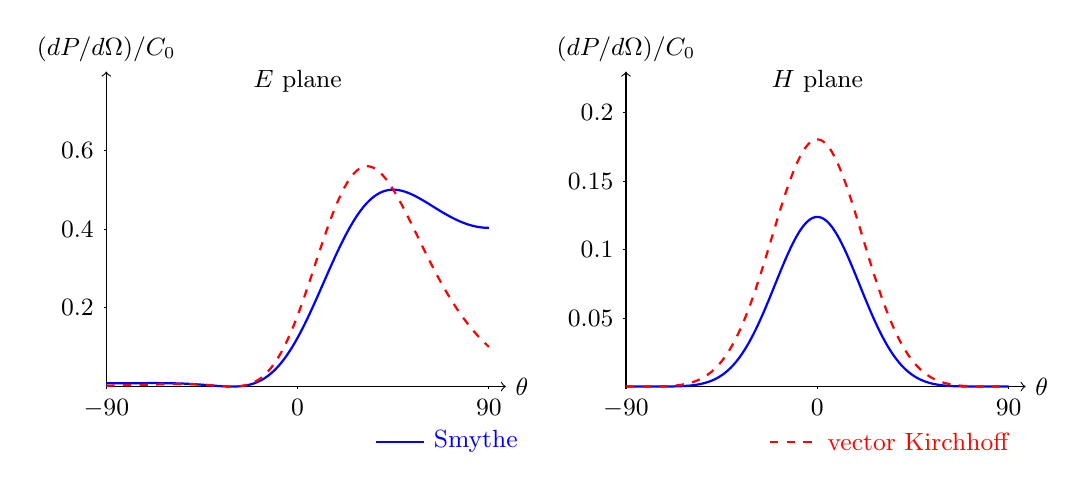
\begin{tikzpicture}[font=\small]
\begin{scope}[shift={(0cm,0)},x=.027cm,y=5.0cm]
\draw[->] (-90,0) -- (98,0) node[right] {$\theta$};
\draw[->] (-90,0) -- (-90,0.8) node[above] {$(dP/d\Omega)/C_0$};
\draw (-90,0) -- ++(0,-0.035cm) node[below] {$-90$};
\draw (0,0) -- ++(0,-0.035cm) node[below] {$0$};
\draw (90,0) -- ++(0,-0.035cm) node[below] {$90$};
\draw (-90,0.2) -- ++(-0.035cm,0) node[left] {$0.2$};
\draw (-90,0.4) -- ++(-0.035cm,0) node[left] {$0.4$};
\draw (-90,0.6) -- ++(-0.035cm,0) node[left] {$0.6$};
\draw[blue,thick] plot coordinates {(-90.00000,0.008323) (-89.70000,0.008323) (-89.40000,0.008323) (-89.10000,0.008324) (-88.80000,0.008325) (-88.50000,0.008327) (-88.20000,0.008328) (-87.90000,0.008330) (-87.60000,0.008333) (-87.30000,0.008335) (-87.00000,0.008338) (-86.70000,0.008341) (-86.40000,0.008345) (-86.10000,0.008349) (-85.80000,0.008353) (-85.50000,0.008357) (-85.20000,0.008362) (-84.90000,0.008366) (-84.60000,0.008372) (-84.30000,0.008377) (-84.00000,0.008383) (-83.70000,0.008389) (-83.40000,0.008395) (-83.10000,0.008401) (-82.80000,0.008408) (-82.50000,0.008415) (-82.20000,0.008422) (-81.90000,0.008429) (-81.60000,0.008436) (-81.30000,0.008444) (-81.00000,0.008452) (-80.70000,0.008460) (-80.40000,0.008468) (-80.10000,0.008476) (-79.80000,0.008484) (-79.50000,0.008493) (-79.20000,0.008501) (-78.90000,0.008510) (-78.60000,0.008519) (-78.30000,0.008528) (-78.00000,0.008537) (-77.70000,0.008546) (-77.40000,0.008555) (-77.10000,0.008564) (-76.80000,0.008573) (-76.50000,0.008582) (-76.20000,0.008591) (-75.90000,0.008599) (-75.60000,0.008608) (-75.30000,0.008617) (-75.00000,0.008626) (-74.70000,0.008634) (-74.40000,0.008643) (-74.10000,0.008651) (-73.80000,0.008659) (-73.50000,0.008667) (-73.20000,0.008674) (-72.90000,0.008682) (-72.60000,0.008689) (-72.30000,0.008696) (-72.00000,0.008702) (-71.70000,0.008708) (-71.40000,0.008714) (-71.10000,0.008720) (-70.80000,0.008725) (-70.50000,0.008730) (-70.20000,0.008734) (-69.90000,0.008738) (-69.60000,0.008741) (-69.30000,0.008744) (-69.00000,0.008746) (-68.70000,0.008747) (-68.40000,0.008749) (-68.10000,0.008749) (-67.80000,0.008749) (-67.50000,0.008748) (-67.20000,0.008746) (-66.90000,0.008744) (-66.60000,0.008740) (-66.30000,0.008737) (-66.00000,0.008732) (-65.70000,0.008726) (-65.40000,0.008719) (-65.10000,0.008712) (-64.80000,0.008704) (-64.50000,0.008694) (-64.20000,0.008684) (-63.90000,0.008672) (-63.60000,0.008660) (-63.30000,0.008646) (-63.00000,0.008631) (-62.70000,0.008615) (-62.40000,0.008598) (-62.10000,0.008579) (-61.80000,0.008560) (-61.50000,0.008539) (-61.20000,0.008516) (-60.90000,0.008493) (-60.60000,0.008467) (-60.30000,0.008441) (-60.00000,0.008413) (-59.70000,0.008383) (-59.40000,0.008352) (-59.10000,0.008320) (-58.80000,0.008285) (-58.50000,0.008250) (-58.20000,0.008212) (-57.90000,0.008173) (-57.60000,0.008132) (-57.30000,0.008090) (-57.00000,0.008045) (-56.70000,0.007999) (-56.40000,0.007952) (-56.10000,0.007902) (-55.80000,0.007850) (-55.50000,0.007797) (-55.20000,0.007742) (-54.90000,0.007684) (-54.60000,0.007625) (-54.30000,0.007564) (-54.00000,0.007501) (-53.70000,0.007436) (-53.40000,0.007369) (-53.10000,0.007300) (-52.80000,0.007229) (-52.50000,0.007156) (-52.20000,0.007080) (-51.90000,0.007003) (-51.60000,0.006924) (-51.30000,0.006843) (-51.00000,0.006760) (-50.70000,0.006674) (-50.40000,0.006587) (-50.10000,0.006498) (-49.80000,0.006406) (-49.50000,0.006313) (-49.20000,0.006218) (-48.90000,0.006120) (-48.60000,0.006021) (-48.30000,0.005920) (-48.00000,0.005817) (-47.70000,0.005712) (-47.40000,0.005606) (-47.10000,0.005497) (-46.80000,0.005387) (-46.50000,0.005276) (-46.20000,0.005162) (-45.90000,0.005047) (-45.60000,0.004931) (-45.30000,0.004813) (-45.00000,0.004694) (-44.70000,0.004573) (-44.40000,0.004451) (-44.10000,0.004328) (-43.80000,0.004204) (-43.50000,0.004079) (-43.20000,0.003954) (-42.90000,0.003827) (-42.60000,0.003700) (-42.30000,0.003572) (-42.00000,0.003443) (-41.70000,0.003315) (-41.40000,0.003186) (-41.10000,0.003057) (-40.80000,0.002928) (-40.50000,0.002799) (-40.20000,0.002671) (-39.90000,0.002543) (-39.60000,0.002416) (-39.30000,0.002290) (-39.00000,0.002165) (-38.70000,0.002041) (-38.40000,0.001918) (-38.10000,0.001797) (-37.80000,0.001678) (-37.50000,0.001561) (-37.20000,0.001446) (-36.90000,0.001334) (-36.60000,0.001224) (-36.30000,0.001117) (-36.00000,0.001013) (-35.70000,0.000913) (-35.40000,0.000816) (-35.10000,0.000723) (-34.80000,0.000635) (-34.50000,0.000550) (-34.20000,0.000471) (-33.90000,0.000397) (-33.60000,0.000328) (-33.30000,0.000264) (-33.00000,0.000207) (-32.70000,0.000156) (-32.40000,0.000111) (-32.10000,0.000074) (-31.80000,0.000044) (-31.50000,0.000021) (-31.20000,0.000006) (-30.90000,0.000000) (-30.60000,0.000003) (-30.30000,0.000014) (-30.00000,0.000035) (-29.70000,0.000067) (-29.40000,0.000108) (-29.10000,0.000160) (-28.80000,0.000223) (-28.50000,0.000297) (-28.20000,0.000384) (-27.90000,0.000483) (-27.60000,0.000595) (-27.30000,0.000719) (-27.00000,0.000858) (-26.70000,0.001011) (-26.40000,0.001178) (-26.10000,0.001360) (-25.80000,0.001558) (-25.50000,0.001772) (-25.20000,0.002002) (-24.90000,0.002249) (-24.60000,0.002514) (-24.30000,0.002796) (-24.00000,0.003097) (-23.70000,0.003416) (-23.40000,0.003755) (-23.10000,0.004114) (-22.80000,0.004493) (-22.50000,0.004893) (-22.20000,0.005314) (-21.90000,0.005757) (-21.60000,0.006222) (-21.30000,0.006710) (-21.00000,0.007222) (-20.70000,0.007757) (-20.40000,0.008317) (-20.10000,0.008901) (-19.80000,0.009510) (-19.50000,0.010146) (-19.20000,0.010807) (-18.90000,0.011496) (-18.60000,0.012211) (-18.30000,0.012954) (-18.00000,0.013726) (-17.70000,0.014526) (-17.40000,0.015355) (-17.10000,0.016214) (-16.80000,0.017103) (-16.50000,0.018022) (-16.20000,0.018973) (-15.90000,0.019954) (-15.60000,0.020968) (-15.30000,0.022014) (-15.00000,0.023092) (-14.70000,0.024203) (-14.40000,0.025348) (-14.10000,0.026526) (-13.80000,0.027739) (-13.50000,0.028986) (-13.20000,0.030268) (-12.90000,0.031586) (-12.60000,0.032938) (-12.30000,0.034327) (-12.00000,0.035752) (-11.70000,0.037213) (-11.40000,0.038711) (-11.10000,0.040246) (-10.80000,0.041819) (-10.50000,0.043428) (-10.20000,0.045076) (-9.90000,0.046761) (-9.60000,0.048484) (-9.30000,0.050246) (-9.00000,0.052046) (-8.70000,0.053884) (-8.40000,0.055761) (-8.10000,0.057677) (-7.80000,0.059631) (-7.50000,0.061625) (-7.20000,0.063657) (-6.90000,0.065728) (-6.60000,0.067838) (-6.30000,0.069988) (-6.00000,0.072175) (-5.70000,0.074402) (-5.40000,0.076668) (-5.10000,0.078972) (-4.80000,0.081315) (-4.50000,0.083696) (-4.20000,0.086115) (-3.90000,0.088572) (-3.60000,0.091068) (-3.30000,0.093601) (-3.00000,0.096171) (-2.70000,0.098778) (-2.40000,0.101422) (-2.10000,0.104103) (-1.80000,0.106820) (-1.50000,0.109573) (-1.20000,0.112361) (-0.90000,0.115185) (-0.60000,0.118043) (-0.30000,0.120935) (0.00000,0.123861) (0.30000,0.126821) (0.60000,0.129813) (0.90000,0.132837) (1.20000,0.135893) (1.50000,0.138981) (1.80000,0.142099) (2.10000,0.145247) (2.40000,0.148424) (2.70000,0.151630) (3.00000,0.154864) (3.30000,0.158126) (3.60000,0.161414) (3.90000,0.164729) (4.20000,0.168068) (4.50000,0.171432) (4.80000,0.174820) (5.10000,0.178231) (5.40000,0.181664) (5.70000,0.185118) (6.00000,0.188593) (6.30000,0.192087) (6.60000,0.195601) (6.90000,0.199132) (7.20000,0.202680) (7.50000,0.206245) (7.80000,0.209824) (8.10000,0.213418) (8.40000,0.217026) (8.70000,0.220646) (9.00000,0.224277) (9.30000,0.227919) (9.60000,0.231571) (9.90000,0.235231) (10.20000,0.238898) (10.50000,0.242573) (10.80000,0.246253) (11.10000,0.249937) (11.40000,0.253625) (11.70000,0.257316) (12.00000,0.261008) (12.30000,0.264700) (12.60000,0.268393) (12.90000,0.272083) (13.20000,0.275771) (13.50000,0.279456) (13.80000,0.283136) (14.10000,0.286810) (14.40000,0.290478) (14.70000,0.294137) (15.00000,0.297789) (15.30000,0.301430) (15.60000,0.305061) (15.90000,0.308680) (16.20000,0.312286) (16.50000,0.315878) (16.80000,0.319456) (17.10000,0.323018) (17.40000,0.326563) (17.70000,0.330091) (18.00000,0.333600) (18.30000,0.337089) (18.60000,0.340558) (18.90000,0.344006) (19.20000,0.347431) (19.50000,0.350833) (19.80000,0.354211) (20.10000,0.357563) (20.40000,0.360890) (20.70000,0.364190) (21.00000,0.367463) (21.30000,0.370707) (21.60000,0.373922) (21.90000,0.377107) (22.20000,0.380261) (22.50000,0.383384) (22.80000,0.386474) (23.10000,0.389531) (23.40000,0.392555) (23.70000,0.395544) (24.00000,0.398498) (24.30000,0.401417) (24.60000,0.404299) (24.90000,0.407144) (25.20000,0.409952) (25.50000,0.412721) (25.80000,0.415452) (26.10000,0.418144) (26.40000,0.420796) (26.70000,0.423407) (27.00000,0.425978) (27.30000,0.428508) (27.60000,0.430996) (27.90000,0.433442) (28.20000,0.435846) (28.50000,0.438207) (28.80000,0.440525) (29.10000,0.442799) (29.40000,0.445030) (29.70000,0.447217) (30.00000,0.449359) (30.30000,0.451457) (30.60000,0.453511) (30.90000,0.455519) (31.20000,0.457482) (31.50000,0.459400) (31.80000,0.461272) (32.10000,0.463099) (32.40000,0.464880) (32.70000,0.466616) (33.00000,0.468306) (33.30000,0.469950) (33.60000,0.471548) (33.90000,0.473101) (34.20000,0.474607) (34.50000,0.476068) (34.80000,0.477484) (35.10000,0.478853) (35.40000,0.480178) (35.70000,0.481456) (36.00000,0.482690) (36.30000,0.483879) (36.60000,0.485022) (36.90000,0.486121) (37.20000,0.487176) (37.50000,0.488186) (37.80000,0.489152) (38.10000,0.490074) (38.40000,0.490953) (38.70000,0.491789) (39.00000,0.492581) (39.30000,0.493332) (39.60000,0.494039) (39.90000,0.494705) (40.20000,0.495329) (40.50000,0.495913) (40.80000,0.496455) (41.10000,0.496957) (41.40000,0.497418) (41.70000,0.497840) (42.00000,0.498223) (42.30000,0.498568) (42.60000,0.498874) (42.90000,0.499142) (43.20000,0.499372) (43.50000,0.499566) (43.80000,0.499724) (44.10000,0.499845) (44.40000,0.499932) (44.70000,0.499983) (45.00000,0.500000) (45.30000,0.499983) (45.60000,0.499933) (45.90000,0.499850) (46.20000,0.499735) (46.50000,0.499588) (46.80000,0.499411) (47.10000,0.499202) (47.40000,0.498964) (47.70000,0.498696) (48.00000,0.498400) (48.30000,0.498075) (48.60000,0.497723) (48.90000,0.497343) (49.20000,0.496937) (49.50000,0.496506) (49.80000,0.496048) (50.10000,0.495567) (50.40000,0.495061) (50.70000,0.494531) (51.00000,0.493979) (51.30000,0.493404) (51.60000,0.492807) (51.90000,0.492190) (52.20000,0.491551) (52.50000,0.490893) (52.80000,0.490215) (53.10000,0.489519) (53.40000,0.488805) (53.70000,0.488072) (54.00000,0.487323) (54.30000,0.486558) (54.60000,0.485776) (54.90000,0.484979) (55.20000,0.484168) (55.50000,0.483342) (55.80000,0.482503) (56.10000,0.481651) (56.40000,0.480786) (56.70000,0.479910) (57.00000,0.479022) (57.30000,0.478124) (57.60000,0.477215) (57.90000,0.476296) (58.20000,0.475369) (58.50000,0.474432) (58.80000,0.473488) (59.10000,0.472536) (59.40000,0.471577) (59.70000,0.470612) (60.00000,0.469640) (60.30000,0.468663) (60.60000,0.467681) (60.90000,0.466694) (61.20000,0.465703) (61.50000,0.464709) (61.80000,0.463712) (62.10000,0.462712) (62.40000,0.461709) (62.70000,0.460705) (63.00000,0.459700) (63.30000,0.458694) (63.60000,0.457687) (63.90000,0.456681) (64.20000,0.455675) (64.50000,0.454670) (64.80000,0.453666) (65.10000,0.452664) (65.40000,0.451664) (65.70000,0.450666) (66.00000,0.449671) (66.30000,0.448680) (66.60000,0.447692) (66.90000,0.446708) (67.20000,0.445729) (67.50000,0.444754) (67.80000,0.443784) (68.10000,0.442820) (68.40000,0.441862) (68.70000,0.440909) (69.00000,0.439963) (69.30000,0.439024) (69.60000,0.438091) (69.90000,0.437167) (70.20000,0.436249) (70.50000,0.435340) (70.80000,0.434439) (71.10000,0.433546) (71.40000,0.432662) (71.70000,0.431788) (72.00000,0.430922) (72.30000,0.430066) (72.60000,0.429220) (72.90000,0.428384) (73.20000,0.427559) (73.50000,0.426744) (73.80000,0.425939) (74.10000,0.425146) (74.40000,0.424364) (74.70000,0.423594) (75.00000,0.422835) (75.30000,0.422088) (75.60000,0.421353) (75.90000,0.420631) (76.20000,0.419921) (76.50000,0.419223) (76.80000,0.418539) (77.10000,0.417867) (77.40000,0.417208) (77.70000,0.416563) (78.00000,0.415932) (78.30000,0.415314) (78.60000,0.414710) (78.90000,0.414120) (79.20000,0.413543) (79.50000,0.412982) (79.80000,0.412434) (80.10000,0.411901) (80.40000,0.411383) (80.70000,0.410879) (81.00000,0.410391) (81.30000,0.409917) (81.60000,0.409458) (81.90000,0.409015) (82.20000,0.408586) (82.50000,0.408173) (82.80000,0.407776) (83.10000,0.407394) (83.40000,0.407028) (83.70000,0.406678) (84.00000,0.406343) (84.30000,0.406024) (84.60000,0.405721) (84.90000,0.405435) (85.20000,0.405164) (85.50000,0.404909) (85.80000,0.404671) (86.10000,0.404448) (86.40000,0.404243) (86.70000,0.404053) (87.00000,0.403880) (87.30000,0.403723) (87.60000,0.403582) (87.90000,0.403458) (88.20000,0.403351) (88.50000,0.403260) (88.80000,0.403185) (89.10000,0.403127) (89.40000,0.403086) (89.70000,0.403061) (90.00000,0.403053)};
\draw[red,dashed,thick] plot coordinates {(-90.00000,0.002081) (-89.70000,0.002112) (-89.40000,0.002143) (-89.10000,0.002174) (-88.80000,0.002206) (-88.50000,0.002239) (-88.20000,0.002271) (-87.90000,0.002304) (-87.60000,0.002337) (-87.30000,0.002371) (-87.00000,0.002404) (-86.70000,0.002439) (-86.40000,0.002473) (-86.10000,0.002508) (-85.80000,0.002543) (-85.50000,0.002579) (-85.20000,0.002614) (-84.90000,0.002651) (-84.60000,0.002687) (-84.30000,0.002724) (-84.00000,0.002761) (-83.70000,0.002799) (-83.40000,0.002836) (-83.10000,0.002875) (-82.80000,0.002913) (-82.50000,0.002952) (-82.20000,0.002991) (-81.90000,0.003031) (-81.60000,0.003071) (-81.30000,0.003111) (-81.00000,0.003151) (-80.70000,0.003192) (-80.40000,0.003233) (-80.10000,0.003275) (-79.80000,0.003317) (-79.50000,0.003359) (-79.20000,0.003401) (-78.90000,0.003444) (-78.60000,0.003487) (-78.30000,0.003530) (-78.00000,0.003574) (-77.70000,0.003618) (-77.40000,0.003662) (-77.10000,0.003706) (-76.80000,0.003751) (-76.50000,0.003796) (-76.20000,0.003841) (-75.90000,0.003886) (-75.60000,0.003932) (-75.30000,0.003978) (-75.00000,0.004024) (-74.70000,0.004070) (-74.40000,0.004117) (-74.10000,0.004163) (-73.80000,0.004210) (-73.50000,0.004257) (-73.20000,0.004304) (-72.90000,0.004351) (-72.60000,0.004398) (-72.30000,0.004445) (-72.00000,0.004493) (-71.70000,0.004540) (-71.40000,0.004587) (-71.10000,0.004635) (-70.80000,0.004682) (-70.50000,0.004729) (-70.20000,0.004777) (-69.90000,0.004824) (-69.60000,0.004871) (-69.30000,0.004918) (-69.00000,0.004964) (-68.70000,0.005011) (-68.40000,0.005057) (-68.10000,0.005103) (-67.80000,0.005149) (-67.50000,0.005195) (-67.20000,0.005240) (-66.90000,0.005285) (-66.60000,0.005329) (-66.30000,0.005373) (-66.00000,0.005416) (-65.70000,0.005460) (-65.40000,0.005502) (-65.10000,0.005544) (-64.80000,0.005585) (-64.50000,0.005626) (-64.20000,0.005666) (-63.90000,0.005705) (-63.60000,0.005744) (-63.30000,0.005781) (-63.00000,0.005818) (-62.70000,0.005854) (-62.40000,0.005889) (-62.10000,0.005923) (-61.80000,0.005956) (-61.50000,0.005988) (-61.20000,0.006018) (-60.90000,0.006048) (-60.60000,0.006076) (-60.30000,0.006103) (-60.00000,0.006129) (-59.70000,0.006154) (-59.40000,0.006177) (-59.10000,0.006198) (-58.80000,0.006218) (-58.50000,0.006236) (-58.20000,0.006253) (-57.90000,0.006268) (-57.60000,0.006282) (-57.30000,0.006293) (-57.00000,0.006303) (-56.70000,0.006311) (-56.40000,0.006317) (-56.10000,0.006321) (-55.80000,0.006323) (-55.50000,0.006323) (-55.20000,0.006320) (-54.90000,0.006316) (-54.60000,0.006309) (-54.30000,0.006300) (-54.00000,0.006289) (-53.70000,0.006275) (-53.40000,0.006259) (-53.10000,0.006240) (-52.80000,0.006219) (-52.50000,0.006195) (-52.20000,0.006169) (-51.90000,0.006140) (-51.60000,0.006108) (-51.30000,0.006074) (-51.00000,0.006036) (-50.70000,0.005996) (-50.40000,0.005954) (-50.10000,0.005908) (-49.80000,0.005860) (-49.50000,0.005809) (-49.20000,0.005755) (-48.90000,0.005698) (-48.60000,0.005638) (-48.30000,0.005575) (-48.00000,0.005509) (-47.70000,0.005440) (-47.40000,0.005369) (-47.10000,0.005294) (-46.80000,0.005217) (-46.50000,0.005137) (-46.20000,0.005054) (-45.90000,0.004968) (-45.60000,0.004879) (-45.30000,0.004788) (-45.00000,0.004694) (-44.70000,0.004597) (-44.40000,0.004498) (-44.10000,0.004396) (-43.80000,0.004292) (-43.50000,0.004186) (-43.20000,0.004077) (-42.90000,0.003966) (-42.60000,0.003853) (-42.30000,0.003738) (-42.00000,0.003621) (-41.70000,0.003503) (-41.40000,0.003383) (-41.10000,0.003261) (-40.80000,0.003138) (-40.50000,0.003014) (-40.20000,0.002890) (-39.90000,0.002764) (-39.60000,0.002638) (-39.30000,0.002511) (-39.00000,0.002385) (-38.70000,0.002258) (-38.40000,0.002132) (-38.10000,0.002006) (-37.80000,0.001881) (-37.50000,0.001757) (-37.20000,0.001635) (-36.90000,0.001514) (-36.60000,0.001395) (-36.30000,0.001278) (-36.00000,0.001164) (-35.70000,0.001053) (-35.40000,0.000945) (-35.10000,0.000841) (-34.80000,0.000741) (-34.50000,0.000645) (-34.20000,0.000554) (-33.90000,0.000469) (-33.60000,0.000389) (-33.30000,0.000315) (-33.00000,0.000247) (-32.70000,0.000187) (-32.40000,0.000134) (-32.10000,0.000089) (-31.80000,0.000053) (-31.50000,0.000026) (-31.20000,0.000008) (-30.90000,0.000000) (-30.60000,0.000003) (-30.30000,0.000018) (-30.00000,0.000044) (-29.70000,0.000083) (-29.40000,0.000134) (-29.10000,0.000200) (-28.80000,0.000279) (-28.50000,0.000374) (-28.20000,0.000484) (-27.90000,0.000611) (-27.60000,0.000755) (-27.30000,0.000916) (-27.00000,0.001096) (-26.70000,0.001295) (-26.40000,0.001513) (-26.10000,0.001752) (-25.80000,0.002013) (-25.50000,0.002296) (-25.20000,0.002601) (-24.90000,0.002930) (-24.60000,0.003284) (-24.30000,0.003662) (-24.00000,0.004067) (-23.70000,0.004498) (-23.40000,0.004957) (-23.10000,0.005445) (-22.80000,0.005961) (-22.50000,0.006508) (-22.20000,0.007085) (-21.90000,0.007694) (-21.60000,0.008336) (-21.30000,0.009011) (-21.00000,0.009720) (-20.70000,0.010464) (-20.40000,0.011244) (-20.10000,0.012060) (-19.80000,0.012914) (-19.50000,0.013807) (-19.20000,0.014738) (-18.90000,0.015709) (-18.60000,0.016721) (-18.30000,0.017774) (-18.00000,0.018870) (-17.70000,0.020008) (-17.40000,0.021191) (-17.10000,0.022418) (-16.80000,0.023690) (-16.50000,0.025009) (-16.20000,0.026374) (-15.90000,0.027787) (-15.60000,0.029248) (-15.30000,0.030758) (-15.00000,0.032317) (-14.70000,0.033927) (-14.40000,0.035588) (-14.10000,0.037299) (-13.80000,0.039063) (-13.50000,0.040880) (-13.20000,0.042750) (-12.90000,0.044673) (-12.60000,0.046650) (-12.30000,0.048682) (-12.00000,0.050769) (-11.70000,0.052912) (-11.40000,0.055110) (-11.10000,0.057365) (-10.80000,0.059676) (-10.50000,0.062044) (-10.20000,0.064470) (-9.90000,0.066952) (-9.60000,0.069492) (-9.30000,0.072090) (-9.00000,0.074746) (-8.70000,0.077460) (-8.40000,0.080232) (-8.10000,0.083062) (-7.80000,0.085950) (-7.50000,0.088896) (-7.20000,0.091900) (-6.90000,0.094962) (-6.60000,0.098082) (-6.30000,0.101259) (-6.00000,0.104494) (-5.70000,0.107785) (-5.40000,0.111133) (-5.10000,0.114537) (-4.80000,0.117998) (-4.50000,0.121514) (-4.20000,0.125084) (-3.90000,0.128710) (-3.60000,0.132389) (-3.30000,0.136121) (-3.00000,0.139906) (-2.70000,0.143743) (-2.40000,0.147631) (-2.10000,0.151570) (-1.80000,0.155558) (-1.50000,0.159595) (-1.20000,0.163680) (-0.90000,0.167812) (-0.60000,0.171990) (-0.30000,0.176212) (0.00000,0.180479) (0.30000,0.184788) (0.60000,0.189139) (0.90000,0.193530) (1.20000,0.197960) (1.50000,0.202428) (1.80000,0.206933) (2.10000,0.211473) (2.40000,0.216048) (2.70000,0.220654) (3.00000,0.225292) (3.30000,0.229959) (3.60000,0.234654) (3.90000,0.239376) (4.20000,0.244123) (4.50000,0.248894) (4.80000,0.253686) (5.10000,0.258498) (5.40000,0.263329) (5.70000,0.268176) (6.00000,0.273039) (6.30000,0.277915) (6.60000,0.282802) (6.90000,0.287700) (7.20000,0.292605) (7.50000,0.297516) (7.80000,0.302432) (8.10000,0.307349) (8.40000,0.312268) (8.70000,0.317185) (9.00000,0.322099) (9.30000,0.327008) (9.60000,0.331910) (9.90000,0.336803) (10.20000,0.341685) (10.50000,0.346554) (10.80000,0.351409) (11.10000,0.356247) (11.40000,0.361066) (11.70000,0.365865) (12.00000,0.370642) (12.30000,0.375394) (12.60000,0.380120) (12.90000,0.384818) (13.20000,0.389486) (13.50000,0.394122) (13.80000,0.398725) (14.10000,0.403292) (14.40000,0.407821) (14.70000,0.412312) (15.00000,0.416761) (15.30000,0.421167) (15.60000,0.425529) (15.90000,0.429845) (16.20000,0.434112) (16.50000,0.438330) (16.80000,0.442497) (17.10000,0.446611) (17.40000,0.450670) (17.70000,0.454672) (18.00000,0.458617) (18.30000,0.462503) (18.60000,0.466329) (18.90000,0.470092) (19.20000,0.473791) (19.50000,0.477426) (19.80000,0.480994) (20.10000,0.484494) (20.40000,0.487926) (20.70000,0.491288) (21.00000,0.494578) (21.30000,0.497796) (21.60000,0.500941) (21.90000,0.504011) (22.20000,0.507005) (22.50000,0.509923) (22.80000,0.512763) (23.10000,0.515524) (23.40000,0.518207) (23.70000,0.520809) (24.00000,0.523331) (24.30000,0.525771) (24.60000,0.528129) (24.90000,0.530404) (25.20000,0.532595) (25.50000,0.534703) (25.80000,0.536726) (26.10000,0.538664) (26.40000,0.540518) (26.70000,0.542285) (27.00000,0.543967) (27.30000,0.545562) (27.60000,0.547071) (27.90000,0.548494) (28.20000,0.549830) (28.50000,0.551079) (28.80000,0.552242) (29.10000,0.553317) (29.40000,0.554306) (29.70000,0.555209) (30.00000,0.556025) (30.30000,0.556755) (30.60000,0.557398) (30.90000,0.557956) (31.20000,0.558429) (31.50000,0.558816) (31.80000,0.559119) (32.10000,0.559337) (32.40000,0.559472) (32.70000,0.559523) (33.00000,0.559492) (33.30000,0.559378) (33.60000,0.559182) (33.90000,0.558906) (34.20000,0.558549) (34.50000,0.558113) (34.80000,0.557597) (35.10000,0.557004) (35.40000,0.556333) (35.70000,0.555586) (36.00000,0.554763) (36.30000,0.553866) (36.60000,0.552894) (36.90000,0.551850) (37.20000,0.550733) (37.50000,0.549546) (37.80000,0.548289) (38.10000,0.546962) (38.40000,0.545568) (38.70000,0.544107) (39.00000,0.542580) (39.30000,0.540988) (39.60000,0.539333) (39.90000,0.537615) (40.20000,0.535836) (40.50000,0.533997) (40.80000,0.532099) (41.10000,0.530143) (41.40000,0.528130) (41.70000,0.526062) (42.00000,0.523939) (42.30000,0.521764) (42.60000,0.519536) (42.90000,0.517258) (43.20000,0.514931) (43.50000,0.512556) (43.80000,0.510133) (44.10000,0.507665) (44.40000,0.505153) (44.70000,0.502597) (45.00000,0.500000) (45.30000,0.497362) (45.60000,0.494684) (45.90000,0.491969) (46.20000,0.489216) (46.50000,0.486427) (46.80000,0.483604) (47.10000,0.480748) (47.40000,0.477860) (47.70000,0.474941) (48.00000,0.471992) (48.30000,0.469015) (48.60000,0.466010) (48.90000,0.462980) (49.20000,0.459924) (49.50000,0.456845) (49.80000,0.453743) (50.10000,0.450620) (50.40000,0.447476) (50.70000,0.444313) (51.00000,0.441132) (51.30000,0.437934) (51.60000,0.434720) (51.90000,0.431491) (52.20000,0.428248) (52.50000,0.424993) (52.80000,0.421726) (53.10000,0.418447) (53.40000,0.415160) (53.70000,0.411863) (54.00000,0.408558) (54.30000,0.405247) (54.60000,0.401930) (54.90000,0.398607) (55.20000,0.395281) (55.50000,0.391951) (55.80000,0.388619) (56.10000,0.385285) (56.40000,0.381950) (56.70000,0.378616) (57.00000,0.375282) (57.30000,0.371950) (57.60000,0.368621) (57.90000,0.365294) (58.20000,0.361972) (58.50000,0.358654) (58.80000,0.355342) (59.10000,0.352035) (59.40000,0.348735) (59.70000,0.345443) (60.00000,0.342158) (60.30000,0.338882) (60.60000,0.335615) (60.90000,0.332357) (61.20000,0.329110) (61.50000,0.325874) (61.80000,0.322649) (62.10000,0.319436) (62.40000,0.316235) (62.70000,0.313046) (63.00000,0.309872) (63.30000,0.306710) (63.60000,0.303563) (63.90000,0.300431) (64.20000,0.297313) (64.50000,0.294211) (64.80000,0.291124) (65.10000,0.288054) (65.40000,0.285000) (65.70000,0.281962) (66.00000,0.278942) (66.30000,0.275939) (66.60000,0.272953) (66.90000,0.269985) (67.20000,0.267036) (67.50000,0.264104) (67.80000,0.261192) (68.10000,0.258298) (68.40000,0.255423) (68.70000,0.252567) (69.00000,0.249731) (69.30000,0.246914) (69.60000,0.244117) (69.90000,0.241340) (70.20000,0.238583) (70.50000,0.235846) (70.80000,0.233129) (71.10000,0.230432) (71.40000,0.227756) (71.70000,0.225100) (72.00000,0.222465) (72.30000,0.219851) (72.60000,0.217257) (72.90000,0.214684) (73.20000,0.212132) (73.50000,0.209600) (73.80000,0.207089) (74.10000,0.204600) (74.40000,0.202131) (74.70000,0.199683) (75.00000,0.197255) (75.30000,0.194849) (75.60000,0.192463) (75.90000,0.190098) (76.20000,0.187754) (76.50000,0.185430) (76.80000,0.183128) (77.10000,0.180845) (77.40000,0.178583) (77.70000,0.176342) (78.00000,0.174121) (78.30000,0.171921) (78.60000,0.169740) (78.90000,0.167580) (79.20000,0.165440) (79.50000,0.163320) (79.80000,0.161219) (80.10000,0.159139) (80.40000,0.157078) (80.70000,0.155037) (81.00000,0.153015) (81.30000,0.151012) (81.60000,0.149029) (81.90000,0.147065) (82.20000,0.145120) (82.50000,0.143193) (82.80000,0.141286) (83.10000,0.139396) (83.40000,0.137526) (83.70000,0.135674) (84.00000,0.133840) (84.30000,0.132024) (84.60000,0.130226) (84.90000,0.128445) (85.20000,0.126683) (85.50000,0.124938) (85.80000,0.123210) (86.10000,0.121499) (86.40000,0.119806) (86.70000,0.118129) (87.00000,0.116469) (87.30000,0.114826) (87.60000,0.113200) (87.90000,0.111589) (88.20000,0.109995) (88.50000,0.108417) (88.80000,0.106855) (89.10000,0.105309) (89.40000,0.103778) (89.70000,0.102263) (90.00000,0.100763)};
\node at (0,0.776) {$E$ plane};
\end{scope}
\begin{scope}[shift={(6.6cm,0)},x=.027cm,y=17.391304347826086cm]
\draw[->] (-90,0) -- (98,0) node[right] {$\theta$};
\draw[->] (-90,0) -- (-90,0.23) node[above] {$(dP/d\Omega)/C_0$};
\draw (-90,0) -- ++(0,-0.035cm) node[below] {$-90$};
\draw (0,0) -- ++(0,-0.035cm) node[below] {$0$};
\draw (90,0) -- ++(0,-0.035cm) node[below] {$90$};
\draw (-90,0.05) -- ++(-0.035cm,0) node[left] {$0.05$};
\draw (-90,0.1) -- ++(-0.035cm,0) node[left] {$0.1$};
\draw (-90,0.15) -- ++(-0.035cm,0) node[left] {$0.15$};
\draw (-90,0.2) -- ++(-0.035cm,0) node[left] {$0.2$};
\draw[blue,thick] plot coordinates {(-90.00000,0.000000) (-89.70000,0.000000) (-89.40000,0.000000) (-89.10000,0.000000) (-88.80000,0.000000) (-88.50000,0.000000) (-88.20000,0.000000) (-87.90000,0.000000) (-87.60000,0.000000) (-87.30000,0.000000) (-87.00000,0.000000) (-86.70000,0.000000) (-86.40000,0.000000) (-86.10000,0.000000) (-85.80000,0.000000) (-85.50000,0.000000) (-85.20000,0.000000) (-84.90000,0.000000) (-84.60000,0.000000) (-84.30000,0.000000) (-84.00000,0.000000) (-83.70000,0.000000) (-83.40000,0.000000) (-83.10000,0.000000) (-82.80000,0.000000) (-82.50000,0.000000) (-82.20000,0.000000) (-81.90000,0.000000) (-81.60000,0.000000) (-81.30000,0.000000) (-81.00000,0.000000) (-80.70000,0.000000) (-80.40000,0.000000) (-80.10000,0.000000) (-79.80000,0.000000) (-79.50000,0.000001) (-79.20000,0.000001) (-78.90000,0.000001) (-78.60000,0.000001) (-78.30000,0.000001) (-78.00000,0.000002) (-77.70000,0.000002) (-77.40000,0.000002) (-77.10000,0.000003) (-76.80000,0.000003) (-76.50000,0.000004) (-76.20000,0.000004) (-75.90000,0.000005) (-75.60000,0.000006) (-75.30000,0.000007) (-75.00000,0.000008) (-74.70000,0.000009) (-74.40000,0.000010) (-74.10000,0.000012) (-73.80000,0.000013) (-73.50000,0.000015) (-73.20000,0.000017) (-72.90000,0.000019) (-72.60000,0.000022) (-72.30000,0.000024) (-72.00000,0.000027) (-71.70000,0.000030) (-71.40000,0.000034) (-71.10000,0.000037) (-70.80000,0.000041) (-70.50000,0.000046) (-70.20000,0.000050) (-69.90000,0.000056) (-69.60000,0.000061) (-69.30000,0.000067) (-69.00000,0.000074) (-68.70000,0.000081) (-68.40000,0.000089) (-68.10000,0.000097) (-67.80000,0.000106) (-67.50000,0.000115) (-67.20000,0.000125) (-66.90000,0.000136) (-66.60000,0.000148) (-66.30000,0.000161) (-66.00000,0.000174) (-65.70000,0.000188) (-65.40000,0.000204) (-65.10000,0.000220) (-64.80000,0.000237) (-64.50000,0.000256) (-64.20000,0.000275) (-63.90000,0.000296) (-63.60000,0.000318) (-63.30000,0.000342) (-63.00000,0.000366) (-62.70000,0.000393) (-62.40000,0.000421) (-62.10000,0.000450) (-61.80000,0.000481) (-61.50000,0.000514) (-61.20000,0.000549) (-60.90000,0.000586) (-60.60000,0.000624) (-60.30000,0.000665) (-60.00000,0.000708) (-59.70000,0.000753) (-59.40000,0.000801) (-59.10000,0.000851) (-58.80000,0.000903) (-58.50000,0.000958) (-58.20000,0.001016) (-57.90000,0.001077) (-57.60000,0.001141) (-57.30000,0.001207) (-57.00000,0.001277) (-56.70000,0.001350) (-56.40000,0.001427) (-56.10000,0.001507) (-55.80000,0.001590) (-55.50000,0.001678) (-55.20000,0.001769) (-54.90000,0.001864) (-54.60000,0.001964) (-54.30000,0.002067) (-54.00000,0.002175) (-53.70000,0.002288) (-53.40000,0.002405) (-53.10000,0.002527) (-52.80000,0.002654) (-52.50000,0.002786) (-52.20000,0.002924) (-51.90000,0.003066) (-51.60000,0.003215) (-51.30000,0.003369) (-51.00000,0.003529) (-50.70000,0.003695) (-50.40000,0.003867) (-50.10000,0.004045) (-49.80000,0.004230) (-49.50000,0.004421) (-49.20000,0.004620) (-48.90000,0.004825) (-48.60000,0.005038) (-48.30000,0.005258) (-48.00000,0.005485) (-47.70000,0.005720) (-47.40000,0.005963) (-47.10000,0.006214) (-46.80000,0.006473) (-46.50000,0.006740) (-46.20000,0.007016) (-45.90000,0.007300) (-45.60000,0.007594) (-45.30000,0.007896) (-45.00000,0.008208) (-44.70000,0.008529) (-44.40000,0.008859) (-44.10000,0.009199) (-43.80000,0.009549) (-43.50000,0.009909) (-43.20000,0.010279) (-42.90000,0.010660) (-42.60000,0.011051) (-42.30000,0.011452) (-42.00000,0.011865) (-41.70000,0.012288) (-41.40000,0.012723) (-41.10000,0.013168) (-40.80000,0.013625) (-40.50000,0.014094) (-40.20000,0.014574) (-39.90000,0.015066) (-39.60000,0.015570) (-39.30000,0.016086) (-39.00000,0.016614) (-38.70000,0.017154) (-38.40000,0.017707) (-38.10000,0.018272) (-37.80000,0.018849) (-37.50000,0.019439) (-37.20000,0.020042) (-36.90000,0.020657) (-36.60000,0.021286) (-36.30000,0.021927) (-36.00000,0.022581) (-35.70000,0.023248) (-35.40000,0.023928) (-35.10000,0.024622) (-34.80000,0.025328) (-34.50000,0.026047) (-34.20000,0.026779) (-33.90000,0.027525) (-33.60000,0.028283) (-33.30000,0.029055) (-33.00000,0.029839) (-32.70000,0.030636) (-32.40000,0.031447) (-32.10000,0.032270) (-31.80000,0.033106) (-31.50000,0.033954) (-31.20000,0.034815) (-30.90000,0.035688) (-30.60000,0.036574) (-30.30000,0.037472) (-30.00000,0.038382) (-29.70000,0.039304) (-29.40000,0.040238) (-29.10000,0.041183) (-28.80000,0.042139) (-28.50000,0.043107) (-28.20000,0.044086) (-27.90000,0.045075) (-27.60000,0.046075) (-27.30000,0.047086) (-27.00000,0.048106) (-26.70000,0.049136) (-26.40000,0.050175) (-26.10000,0.051224) (-25.80000,0.052281) (-25.50000,0.053347) (-25.20000,0.054421) (-24.90000,0.055503) (-24.60000,0.056592) (-24.30000,0.057689) (-24.00000,0.058792) (-23.70000,0.059902) (-23.40000,0.061017) (-23.10000,0.062138) (-22.80000,0.063265) (-22.50000,0.064396) (-22.20000,0.065531) (-21.90000,0.066670) (-21.60000,0.067812) (-21.30000,0.068957) (-21.00000,0.070105) (-20.70000,0.071254) (-20.40000,0.072405) (-20.10000,0.073556) (-19.80000,0.074708) (-19.50000,0.075860) (-19.20000,0.077011) (-18.90000,0.078161) (-18.60000,0.079309) (-18.30000,0.080455) (-18.00000,0.081597) (-17.70000,0.082736) (-17.40000,0.083872) (-17.10000,0.085002) (-16.80000,0.086128) (-16.50000,0.087247) (-16.20000,0.088360) (-15.90000,0.089466) (-15.60000,0.090565) (-15.30000,0.091656) (-15.00000,0.092737) (-14.70000,0.093810) (-14.40000,0.094872) (-14.10000,0.095924) (-13.80000,0.096965) (-13.50000,0.097994) (-13.20000,0.099011) (-12.90000,0.100015) (-12.60000,0.101005) (-12.30000,0.101981) (-12.00000,0.102943) (-11.70000,0.103889) (-11.40000,0.104820) (-11.10000,0.105734) (-10.80000,0.106632) (-10.50000,0.107512) (-10.20000,0.108374) (-9.90000,0.109217) (-9.60000,0.110042) (-9.30000,0.110846) (-9.00000,0.111631) (-8.70000,0.112395) (-8.40000,0.113139) (-8.10000,0.113860) (-7.80000,0.114560) (-7.50000,0.115237) (-7.20000,0.115891) (-6.90000,0.116522) (-6.60000,0.117130) (-6.30000,0.117713) (-6.00000,0.118272) (-5.70000,0.118806) (-5.40000,0.119314) (-5.10000,0.119798) (-4.80000,0.120255) (-4.50000,0.120686) (-4.20000,0.121091) (-3.90000,0.121469) (-3.60000,0.121820) (-3.30000,0.122144) (-3.00000,0.122440) (-2.70000,0.122709) (-2.40000,0.122950) (-2.10000,0.123163) (-1.80000,0.123348) (-1.50000,0.123504) (-1.20000,0.123633) (-0.90000,0.123733) (-0.60000,0.123804) (-0.30000,0.123847) (0.00000,0.123861) (0.30000,0.123847) (0.60000,0.123804) (0.90000,0.123733) (1.20000,0.123633) (1.50000,0.123504) (1.80000,0.123348) (2.10000,0.123163) (2.40000,0.122950) (2.70000,0.122709) (3.00000,0.122440) (3.30000,0.122144) (3.60000,0.121820) (3.90000,0.121469) (4.20000,0.121091) (4.50000,0.120686) (4.80000,0.120255) (5.10000,0.119798) (5.40000,0.119314) (5.70000,0.118806) (6.00000,0.118272) (6.30000,0.117713) (6.60000,0.117130) (6.90000,0.116522) (7.20000,0.115891) (7.50000,0.115237) (7.80000,0.114560) (8.10000,0.113860) (8.40000,0.113139) (8.70000,0.112395) (9.00000,0.111631) (9.30000,0.110846) (9.60000,0.110042) (9.90000,0.109217) (10.20000,0.108374) (10.50000,0.107512) (10.80000,0.106632) (11.10000,0.105734) (11.40000,0.104820) (11.70000,0.103889) (12.00000,0.102943) (12.30000,0.101981) (12.60000,0.101005) (12.90000,0.100015) (13.20000,0.099011) (13.50000,0.097994) (13.80000,0.096965) (14.10000,0.095924) (14.40000,0.094872) (14.70000,0.093810) (15.00000,0.092737) (15.30000,0.091656) (15.60000,0.090565) (15.90000,0.089466) (16.20000,0.088360) (16.50000,0.087247) (16.80000,0.086128) (17.10000,0.085002) (17.40000,0.083872) (17.70000,0.082736) (18.00000,0.081597) (18.30000,0.080455) (18.60000,0.079309) (18.90000,0.078161) (19.20000,0.077011) (19.50000,0.075860) (19.80000,0.074708) (20.10000,0.073556) (20.40000,0.072405) (20.70000,0.071254) (21.00000,0.070105) (21.30000,0.068957) (21.60000,0.067812) (21.90000,0.066670) (22.20000,0.065531) (22.50000,0.064396) (22.80000,0.063265) (23.10000,0.062138) (23.40000,0.061017) (23.70000,0.059902) (24.00000,0.058792) (24.30000,0.057689) (24.60000,0.056592) (24.90000,0.055503) (25.20000,0.054421) (25.50000,0.053347) (25.80000,0.052281) (26.10000,0.051224) (26.40000,0.050175) (26.70000,0.049136) (27.00000,0.048106) (27.30000,0.047086) (27.60000,0.046075) (27.90000,0.045075) (28.20000,0.044086) (28.50000,0.043107) (28.80000,0.042139) (29.10000,0.041183) (29.40000,0.040238) (29.70000,0.039304) (30.00000,0.038382) (30.30000,0.037472) (30.60000,0.036574) (30.90000,0.035688) (31.20000,0.034815) (31.50000,0.033954) (31.80000,0.033106) (32.10000,0.032270) (32.40000,0.031447) (32.70000,0.030636) (33.00000,0.029839) (33.30000,0.029055) (33.60000,0.028283) (33.90000,0.027525) (34.20000,0.026779) (34.50000,0.026047) (34.80000,0.025328) (35.10000,0.024622) (35.40000,0.023928) (35.70000,0.023248) (36.00000,0.022581) (36.30000,0.021927) (36.60000,0.021286) (36.90000,0.020657) (37.20000,0.020042) (37.50000,0.019439) (37.80000,0.018849) (38.10000,0.018272) (38.40000,0.017707) (38.70000,0.017154) (39.00000,0.016614) (39.30000,0.016086) (39.60000,0.015570) (39.90000,0.015066) (40.20000,0.014574) (40.50000,0.014094) (40.80000,0.013625) (41.10000,0.013168) (41.40000,0.012723) (41.70000,0.012288) (42.00000,0.011865) (42.30000,0.011452) (42.60000,0.011051) (42.90000,0.010660) (43.20000,0.010279) (43.50000,0.009909) (43.80000,0.009549) (44.10000,0.009199) (44.40000,0.008859) (44.70000,0.008529) (45.00000,0.008208) (45.30000,0.007896) (45.60000,0.007594) (45.90000,0.007300) (46.20000,0.007016) (46.50000,0.006740) (46.80000,0.006473) (47.10000,0.006214) (47.40000,0.005963) (47.70000,0.005720) (48.00000,0.005485) (48.30000,0.005258) (48.60000,0.005038) (48.90000,0.004825) (49.20000,0.004620) (49.50000,0.004421) (49.80000,0.004230) (50.10000,0.004045) (50.40000,0.003867) (50.70000,0.003695) (51.00000,0.003529) (51.30000,0.003369) (51.60000,0.003215) (51.90000,0.003066) (52.20000,0.002924) (52.50000,0.002786) (52.80000,0.002654) (53.10000,0.002527) (53.40000,0.002405) (53.70000,0.002288) (54.00000,0.002175) (54.30000,0.002067) (54.60000,0.001964) (54.90000,0.001864) (55.20000,0.001769) (55.50000,0.001678) (55.80000,0.001590) (56.10000,0.001507) (56.40000,0.001427) (56.70000,0.001350) (57.00000,0.001277) (57.30000,0.001207) (57.60000,0.001141) (57.90000,0.001077) (58.20000,0.001016) (58.50000,0.000958) (58.80000,0.000903) (59.10000,0.000851) (59.40000,0.000801) (59.70000,0.000753) (60.00000,0.000708) (60.30000,0.000665) (60.60000,0.000624) (60.90000,0.000586) (61.20000,0.000549) (61.50000,0.000514) (61.80000,0.000481) (62.10000,0.000450) (62.40000,0.000421) (62.70000,0.000393) (63.00000,0.000366) (63.30000,0.000342) (63.60000,0.000318) (63.90000,0.000296) (64.20000,0.000275) (64.50000,0.000256) (64.80000,0.000237) (65.10000,0.000220) (65.40000,0.000204) (65.70000,0.000188) (66.00000,0.000174) (66.30000,0.000161) (66.60000,0.000148) (66.90000,0.000136) (67.20000,0.000125) (67.50000,0.000115) (67.80000,0.000106) (68.10000,0.000097) (68.40000,0.000089) (68.70000,0.000081) (69.00000,0.000074) (69.30000,0.000067) (69.60000,0.000061) (69.90000,0.000056) (70.20000,0.000050) (70.50000,0.000046) (70.80000,0.000041) (71.10000,0.000037) (71.40000,0.000034) (71.70000,0.000030) (72.00000,0.000027) (72.30000,0.000024) (72.60000,0.000022) (72.90000,0.000019) (73.20000,0.000017) (73.50000,0.000015) (73.80000,0.000013) (74.10000,0.000012) (74.40000,0.000010) (74.70000,0.000009) (75.00000,0.000008) (75.30000,0.000007) (75.60000,0.000006) (75.90000,0.000005) (76.20000,0.000004) (76.50000,0.000004) (76.80000,0.000003) (77.10000,0.000003) (77.40000,0.000002) (77.70000,0.000002) (78.00000,0.000002) (78.30000,0.000001) (78.60000,0.000001) (78.90000,0.000001) (79.20000,0.000001) (79.50000,0.000001) (79.80000,0.000000) (80.10000,0.000000) (80.40000,0.000000) (80.70000,0.000000) (81.00000,0.000000) (81.30000,0.000000) (81.60000,0.000000) (81.90000,0.000000) (82.20000,0.000000) (82.50000,0.000000) (82.80000,0.000000) (83.10000,0.000000) (83.40000,0.000000) (83.70000,0.000000) (84.00000,0.000000) (84.30000,0.000000) (84.60000,0.000000) (84.90000,0.000000) (85.20000,0.000000) (85.50000,0.000000) (85.80000,0.000000) (86.10000,0.000000) (86.40000,0.000000) (86.70000,0.000000) (87.00000,0.000000) (87.30000,0.000000) (87.60000,0.000000) (87.90000,0.000000) (88.20000,0.000000) (88.50000,0.000000) (88.80000,0.000000) (89.10000,0.000000) (89.40000,0.000000) (89.70000,0.000000) (90.00000,0.000000)};
\draw[red,dashed,thick] plot coordinates {(-90.00000,0.000003) (-89.70000,0.000003) (-89.40000,0.000003) (-89.10000,0.000003) (-88.80000,0.000003) (-88.50000,0.000003) (-88.20000,0.000002) (-87.90000,0.000002) (-87.60000,0.000002) (-87.30000,0.000002) (-87.00000,0.000002) (-86.70000,0.000002) (-86.40000,0.000001) (-86.10000,0.000001) (-85.80000,0.000001) (-85.50000,0.000001) (-85.20000,0.000001) (-84.90000,0.000000) (-84.60000,0.000000) (-84.30000,0.000000) (-84.00000,0.000000) (-83.70000,0.000000) (-83.40000,0.000000) (-83.10000,0.000000) (-82.80000,0.000000) (-82.50000,0.000000) (-82.20000,0.000001) (-81.90000,0.000001) (-81.60000,0.000002) (-81.30000,0.000002) (-81.00000,0.000003) (-80.70000,0.000004) (-80.40000,0.000006) (-80.10000,0.000007) (-79.80000,0.000009) (-79.50000,0.000010) (-79.20000,0.000012) (-78.90000,0.000015) (-78.60000,0.000018) (-78.30000,0.000021) (-78.00000,0.000024) (-77.70000,0.000028) (-77.40000,0.000032) (-77.10000,0.000036) (-76.80000,0.000041) (-76.50000,0.000047) (-76.20000,0.000053) (-75.90000,0.000059) (-75.60000,0.000066) (-75.30000,0.000074) (-75.00000,0.000082) (-74.70000,0.000091) (-74.40000,0.000101) (-74.10000,0.000111) (-73.80000,0.000123) (-73.50000,0.000135) (-73.20000,0.000148) (-72.90000,0.000162) (-72.60000,0.000177) (-72.30000,0.000193) (-72.00000,0.000210) (-71.70000,0.000228) (-71.40000,0.000247) (-71.10000,0.000268) (-70.80000,0.000290) (-70.50000,0.000313) (-70.20000,0.000338) (-69.90000,0.000364) (-69.60000,0.000392) (-69.30000,0.000421) (-69.00000,0.000452) (-68.70000,0.000485) (-68.40000,0.000520) (-68.10000,0.000556) (-67.80000,0.000595) (-67.50000,0.000635) (-67.20000,0.000678) (-66.90000,0.000723) (-66.60000,0.000770) (-66.30000,0.000820) (-66.00000,0.000872) (-65.70000,0.000927) (-65.40000,0.000984) (-65.10000,0.001044) (-64.80000,0.001107) (-64.50000,0.001173) (-64.20000,0.001242) (-63.90000,0.001314) (-63.60000,0.001390) (-63.30000,0.001469) (-63.00000,0.001551) (-62.70000,0.001637) (-62.40000,0.001727) (-62.10000,0.001821) (-61.80000,0.001918) (-61.50000,0.002020) (-61.20000,0.002126) (-60.90000,0.002236) (-60.60000,0.002351) (-60.30000,0.002470) (-60.00000,0.002594) (-59.70000,0.002723) (-59.40000,0.002858) (-59.10000,0.002997) (-58.80000,0.003142) (-58.50000,0.003292) (-58.20000,0.003447) (-57.90000,0.003609) (-57.60000,0.003776) (-57.30000,0.003950) (-57.00000,0.004130) (-56.70000,0.004316) (-56.40000,0.004509) (-56.10000,0.004709) (-55.80000,0.004915) (-55.50000,0.005129) (-55.20000,0.005349) (-54.90000,0.005578) (-54.60000,0.005814) (-54.30000,0.006057) (-54.00000,0.006309) (-53.70000,0.006568) (-53.40000,0.006836) (-53.10000,0.007113) (-52.80000,0.007398) (-52.50000,0.007692) (-52.20000,0.007995) (-51.90000,0.008308) (-51.60000,0.008629) (-51.30000,0.008961) (-51.00000,0.009302) (-50.70000,0.009653) (-50.40000,0.010014) (-50.10000,0.010386) (-49.80000,0.010768) (-49.50000,0.011161) (-49.20000,0.011565) (-48.90000,0.011980) (-48.60000,0.012406) (-48.30000,0.012843) (-48.00000,0.013293) (-47.70000,0.013754) (-47.40000,0.014227) (-47.10000,0.014712) (-46.80000,0.015210) (-46.50000,0.015721) (-46.20000,0.016244) (-45.90000,0.016780) (-45.60000,0.017329) (-45.30000,0.017891) (-45.00000,0.018467) (-44.70000,0.019057) (-44.40000,0.019660) (-44.10000,0.020277) (-43.80000,0.020908) (-43.50000,0.021553) (-43.20000,0.022213) (-42.90000,0.022887) (-42.60000,0.023576) (-42.30000,0.024279) (-42.00000,0.024998) (-41.70000,0.025731) (-41.40000,0.026480) (-41.10000,0.027243) (-40.80000,0.028022) (-40.50000,0.028817) (-40.20000,0.029627) (-39.90000,0.030453) (-39.60000,0.031294) (-39.30000,0.032151) (-39.00000,0.033024) (-38.70000,0.033913) (-38.40000,0.034818) (-38.10000,0.035739) (-37.80000,0.036675) (-37.50000,0.037628) (-37.20000,0.038597) (-36.90000,0.039582) (-36.60000,0.040583) (-36.30000,0.041600) (-36.00000,0.042632) (-35.70000,0.043681) (-35.40000,0.044746) (-35.10000,0.045827) (-34.80000,0.046923) (-34.50000,0.048036) (-34.20000,0.049163) (-33.90000,0.050307) (-33.60000,0.051466) (-33.30000,0.052640) (-33.00000,0.053830) (-32.70000,0.055034) (-32.40000,0.056253) (-32.10000,0.057488) (-31.80000,0.058736) (-31.50000,0.059999) (-31.20000,0.061276) (-30.90000,0.062568) (-30.60000,0.063873) (-30.30000,0.065191) (-30.00000,0.066522) (-29.70000,0.067867) (-29.40000,0.069224) (-29.10000,0.070594) (-28.80000,0.071976) (-28.50000,0.073369) (-28.20000,0.074774) (-27.90000,0.076190) (-27.60000,0.077617) (-27.30000,0.079054) (-27.00000,0.080501) (-26.70000,0.081958) (-26.40000,0.083423) (-26.10000,0.084898) (-25.80000,0.086381) (-25.50000,0.087872) (-25.20000,0.089370) (-24.90000,0.090875) (-24.60000,0.092387) (-24.30000,0.093905) (-24.00000,0.095428) (-23.70000,0.096956) (-23.40000,0.098488) (-23.10000,0.100025) (-22.80000,0.101565) (-22.50000,0.103107) (-22.20000,0.104652) (-21.90000,0.106199) (-21.60000,0.107746) (-21.30000,0.109294) (-21.00000,0.110842) (-20.70000,0.112389) (-20.40000,0.113934) (-20.10000,0.115478) (-19.80000,0.117019) (-19.50000,0.118557) (-19.20000,0.120090) (-18.90000,0.121619) (-18.60000,0.123143) (-18.30000,0.124661) (-18.00000,0.126172) (-17.70000,0.127676) (-17.40000,0.129172) (-17.10000,0.130660) (-16.80000,0.132138) (-16.50000,0.133606) (-16.20000,0.135063) (-15.90000,0.136509) (-15.60000,0.137942) (-15.30000,0.139363) (-15.00000,0.140771) (-14.70000,0.142164) (-14.40000,0.143542) (-14.10000,0.144905) (-13.80000,0.146251) (-13.50000,0.147581) (-13.20000,0.148893) (-12.90000,0.150186) (-12.60000,0.151461) (-12.30000,0.152716) (-12.00000,0.153951) (-11.70000,0.155164) (-11.40000,0.156357) (-11.10000,0.157527) (-10.80000,0.158674) (-10.50000,0.159797) (-10.20000,0.160897) (-9.90000,0.161972) (-9.60000,0.163022) (-9.30000,0.164045) (-9.00000,0.165043) (-8.70000,0.166013) (-8.40000,0.166956) (-8.10000,0.167871) (-7.80000,0.168757) (-7.50000,0.169615) (-7.20000,0.170442) (-6.90000,0.171240) (-6.60000,0.172007) (-6.30000,0.172744) (-6.00000,0.173449) (-5.70000,0.174122) (-5.40000,0.174763) (-5.10000,0.175372) (-4.80000,0.175948) (-4.50000,0.176490) (-4.20000,0.176999) (-3.90000,0.177475) (-3.60000,0.177916) (-3.30000,0.178323) (-3.00000,0.178695) (-2.70000,0.179033) (-2.40000,0.179335) (-2.10000,0.179603) (-1.80000,0.179835) (-1.50000,0.180031) (-1.20000,0.180192) (-0.90000,0.180318) (-0.60000,0.180407) (-0.30000,0.180461) (0.00000,0.180479) (0.30000,0.180461) (0.60000,0.180407) (0.90000,0.180318) (1.20000,0.180192) (1.50000,0.180031) (1.80000,0.179835) (2.10000,0.179603) (2.40000,0.179335) (2.70000,0.179033) (3.00000,0.178695) (3.30000,0.178323) (3.60000,0.177916) (3.90000,0.177475) (4.20000,0.176999) (4.50000,0.176490) (4.80000,0.175948) (5.10000,0.175372) (5.40000,0.174763) (5.70000,0.174122) (6.00000,0.173449) (6.30000,0.172744) (6.60000,0.172007) (6.90000,0.171240) (7.20000,0.170442) (7.50000,0.169615) (7.80000,0.168757) (8.10000,0.167871) (8.40000,0.166956) (8.70000,0.166013) (9.00000,0.165043) (9.30000,0.164045) (9.60000,0.163022) (9.90000,0.161972) (10.20000,0.160897) (10.50000,0.159797) (10.80000,0.158674) (11.10000,0.157527) (11.40000,0.156357) (11.70000,0.155164) (12.00000,0.153951) (12.30000,0.152716) (12.60000,0.151461) (12.90000,0.150186) (13.20000,0.148893) (13.50000,0.147581) (13.80000,0.146251) (14.10000,0.144905) (14.40000,0.143542) (14.70000,0.142164) (15.00000,0.140771) (15.30000,0.139363) (15.60000,0.137942) (15.90000,0.136509) (16.20000,0.135063) (16.50000,0.133606) (16.80000,0.132138) (17.10000,0.130660) (17.40000,0.129172) (17.70000,0.127676) (18.00000,0.126172) (18.30000,0.124661) (18.60000,0.123143) (18.90000,0.121619) (19.20000,0.120090) (19.50000,0.118557) (19.80000,0.117019) (20.10000,0.115478) (20.40000,0.113934) (20.70000,0.112389) (21.00000,0.110842) (21.30000,0.109294) (21.60000,0.107746) (21.90000,0.106199) (22.20000,0.104652) (22.50000,0.103107) (22.80000,0.101565) (23.10000,0.100025) (23.40000,0.098488) (23.70000,0.096956) (24.00000,0.095428) (24.30000,0.093905) (24.60000,0.092387) (24.90000,0.090875) (25.20000,0.089370) (25.50000,0.087872) (25.80000,0.086381) (26.10000,0.084898) (26.40000,0.083423) (26.70000,0.081958) (27.00000,0.080501) (27.30000,0.079054) (27.60000,0.077617) (27.90000,0.076190) (28.20000,0.074774) (28.50000,0.073369) (28.80000,0.071976) (29.10000,0.070594) (29.40000,0.069224) (29.70000,0.067867) (30.00000,0.066522) (30.30000,0.065191) (30.60000,0.063873) (30.90000,0.062568) (31.20000,0.061276) (31.50000,0.059999) (31.80000,0.058736) (32.10000,0.057488) (32.40000,0.056253) (32.70000,0.055034) (33.00000,0.053830) (33.30000,0.052640) (33.60000,0.051466) (33.90000,0.050307) (34.20000,0.049163) (34.50000,0.048036) (34.80000,0.046923) (35.10000,0.045827) (35.40000,0.044746) (35.70000,0.043681) (36.00000,0.042632) (36.30000,0.041600) (36.60000,0.040583) (36.90000,0.039582) (37.20000,0.038597) (37.50000,0.037628) (37.80000,0.036675) (38.10000,0.035739) (38.40000,0.034818) (38.70000,0.033913) (39.00000,0.033024) (39.30000,0.032151) (39.60000,0.031294) (39.90000,0.030453) (40.20000,0.029627) (40.50000,0.028817) (40.80000,0.028022) (41.10000,0.027243) (41.40000,0.026480) (41.70000,0.025731) (42.00000,0.024998) (42.30000,0.024279) (42.60000,0.023576) (42.90000,0.022887) (43.20000,0.022213) (43.50000,0.021553) (43.80000,0.020908) (44.10000,0.020277) (44.40000,0.019660) (44.70000,0.019057) (45.00000,0.018467) (45.30000,0.017891) (45.60000,0.017329) (45.90000,0.016780) (46.20000,0.016244) (46.50000,0.015721) (46.80000,0.015210) (47.10000,0.014712) (47.40000,0.014227) (47.70000,0.013754) (48.00000,0.013293) (48.30000,0.012843) (48.60000,0.012406) (48.90000,0.011980) (49.20000,0.011565) (49.50000,0.011161) (49.80000,0.010768) (50.10000,0.010386) (50.40000,0.010014) (50.70000,0.009653) (51.00000,0.009302) (51.30000,0.008961) (51.60000,0.008629) (51.90000,0.008308) (52.20000,0.007995) (52.50000,0.007692) (52.80000,0.007398) (53.10000,0.007113) (53.40000,0.006836) (53.70000,0.006568) (54.00000,0.006309) (54.30000,0.006057) (54.60000,0.005814) (54.90000,0.005578) (55.20000,0.005349) (55.50000,0.005129) (55.80000,0.004915) (56.10000,0.004709) (56.40000,0.004509) (56.70000,0.004316) (57.00000,0.004130) (57.30000,0.003950) (57.60000,0.003776) (57.90000,0.003609) (58.20000,0.003447) (58.50000,0.003292) (58.80000,0.003142) (59.10000,0.002997) (59.40000,0.002858) (59.70000,0.002723) (60.00000,0.002594) (60.30000,0.002470) (60.60000,0.002351) (60.90000,0.002236) (61.20000,0.002126) (61.50000,0.002020) (61.80000,0.001918) (62.10000,0.001821) (62.40000,0.001727) (62.70000,0.001637) (63.00000,0.001551) (63.30000,0.001469) (63.60000,0.001390) (63.90000,0.001314) (64.20000,0.001242) (64.50000,0.001173) (64.80000,0.001107) (65.10000,0.001044) (65.40000,0.000984) (65.70000,0.000927) (66.00000,0.000872) (66.30000,0.000820) (66.60000,0.000770) (66.90000,0.000723) (67.20000,0.000678) (67.50000,0.000635) (67.80000,0.000595) (68.10000,0.000556) (68.40000,0.000520) (68.70000,0.000485) (69.00000,0.000452) (69.30000,0.000421) (69.60000,0.000392) (69.90000,0.000364) (70.20000,0.000338) (70.50000,0.000313) (70.80000,0.000290) (71.10000,0.000268) (71.40000,0.000247) (71.70000,0.000228) (72.00000,0.000210) (72.30000,0.000193) (72.60000,0.000177) (72.90000,0.000162) (73.20000,0.000148) (73.50000,0.000135) (73.80000,0.000123) (74.10000,0.000111) (74.40000,0.000101) (74.70000,0.000091) (75.00000,0.000082) (75.30000,0.000074) (75.60000,0.000066) (75.90000,0.000059) (76.20000,0.000053) (76.50000,0.000047) (76.80000,0.000041) (77.10000,0.000036) (77.40000,0.000032) (77.70000,0.000028) (78.00000,0.000024) (78.30000,0.000021) (78.60000,0.000018) (78.90000,0.000015) (79.20000,0.000012) (79.50000,0.000010) (79.80000,0.000009) (80.10000,0.000007) (80.40000,0.000006) (80.70000,0.000004) (81.00000,0.000003) (81.30000,0.000002) (81.60000,0.000002) (81.90000,0.000001) (82.20000,0.000001) (82.50000,0.000000) (82.80000,0.000000) (83.10000,0.000000) (83.40000,0.000000) (83.70000,0.000000) (84.00000,0.000000) (84.30000,0.000000) (84.60000,0.000000) (84.90000,0.000000) (85.20000,0.000001) (85.50000,0.000001) (85.80000,0.000001) (86.10000,0.000001) (86.40000,0.000001) (86.70000,0.000002) (87.00000,0.000002) (87.30000,0.000002) (87.60000,0.000002) (87.90000,0.000002) (88.20000,0.000002) (88.50000,0.000003) (88.80000,0.000003) (89.10000,0.000003) (89.40000,0.000003) (89.70000,0.000003) (90.00000,0.000003)};
\node at (0,0.2231) {$H$ plane};
\end{scope}
\draw[blue,thick] (1cm,-.7cm)--(1.6cm,-.7cm) node[right] {Smythe};
\draw[red,dashed,thick] (6cm,-.7cm)--(6.6cm,-.7cm) node[right] {vector Kirchhoff};
\end{tikzpicture}
\end{center}

\Needspace{5\baselineskip}
\par\bigskip
\noindent\textbf{10.14}\quad A rectangular opening with sides of length $a$ and $b\geq a$ defined by $x=\pm(a/2)$, $y=\pm(b/2)$ exists in a flat, perfectly conducting plane sheet filling the $x$-$y$ plane. A plane wave is normally incident with its polarization vector making an angle $\beta$ with the long edges of the opening.
\begin{enumerate}
\item[(a)] Calculate the diffracted fields and power per unit solid angle with the vector Smythe--Kirchhoff relation (10.109), assuming that the tangential electric field in the opening is the incident unperturbed field.
\item[(b)] Calculate the corresponding result of the scalar Kirchhoff approximation.
\item[(c)] For $b=a$, $\beta=45^{\circ}$, $ka=4\pi$, compute the vector and scalar approximations to the diffracted power per unit solid angle as a function of the angle $\theta$ for $\phi=0$. Plot a graph showing a comparison between the two results.
\end{enumerate}
\solution
Let $\mathbf e=\sin\beta\,\widehat{\mathbf x}
+\cos\beta\,\widehat{\mathbf y}$, since the long edges run along $y$,
and define $\operatorname{sinc}u=\sin u/u$, continuously equal to one
at zero. The rectangular aperture transform is
\[
{\cal A}(\theta,\phi)=ab\,
\operatorname{sinc}\!\left(\frac{ka}{2}\sin\theta\cos\phi\right)
\operatorname{sinc}\!\left(\frac{kb}{2}\sin\theta\sin\phi\right).
\]
\textbf{(a)} In (10.109),
\[
\boxed{\mathbf E_v=\frac{ikE_0e^{ikr-i\omega t}}{2\pi r}
{\cal A}\,\mathbf n\times(\widehat{\mathbf z}\times\mathbf e),
\qquad \mathbf B_v=\mathbf n\times\mathbf E_v/c.}
\]
The angular distribution is therefore
\[
\boxed{\frac{dP_v}{d\Omega}
=\frac{|E_0|^2 k^2|{\cal A}|^2}{8\pi^2Z_0}
\left[\cos^2\theta+\sin^2\theta\sin^2(\phi+\beta)\right].}
\]
The factor follows from
$|\mathbf n\times(\widehat{\mathbf z}\times\mathbf e)|^2
=\cos^2\theta+(\mathbf n\cdot\mathbf e)^2$.

\textbf{(b)} The scalar field has the same aperture transform, multiplied
by $(1+\cos\theta)/2$ instead of the vector factor, hence
\[
\boxed{\frac{dP_s}{d\Omega}
=\frac{|E_0|^2 k^2|{\cal A}|^2}{8\pi^2Z_0}
\left(\frac{1+\cos\theta}{2}\right)^2.}
\]
Both give the same intensity on axis; the scalar result is independent
of $\beta$.

\textbf{(c)} For the parameters specified, normalize to the common axial
value $P_* = |E_0|^2 k^2a^4/(8\pi^2Z_0)$. Then
\[
\boxed{\frac1{P_*}\frac{dP_v}{d\Omega}
=\frac{1+\cos^2\theta}{2}\operatorname{sinc}^2(2\pi\sin\theta),
\quad
\frac1{P_*}\frac{dP_s}{d\Omega}
=\frac{(1+\cos\theta)^2}{4}\operatorname{sinc}^2(2\pi\sin\theta).}
\]
The common zeros occur at $\theta=30^\circ,90^\circ$.
Their difference is the nonnegative quantity
$\tfrac14(1-\cos\theta)^2\operatorname{sinc}^2(2\pi\sin\theta)$.
At $\theta=45^\circ,60^\circ$ the vector values are
$0.03530,0.01174$ and the scalar values $0.03429,0.01057$.
\begin{center}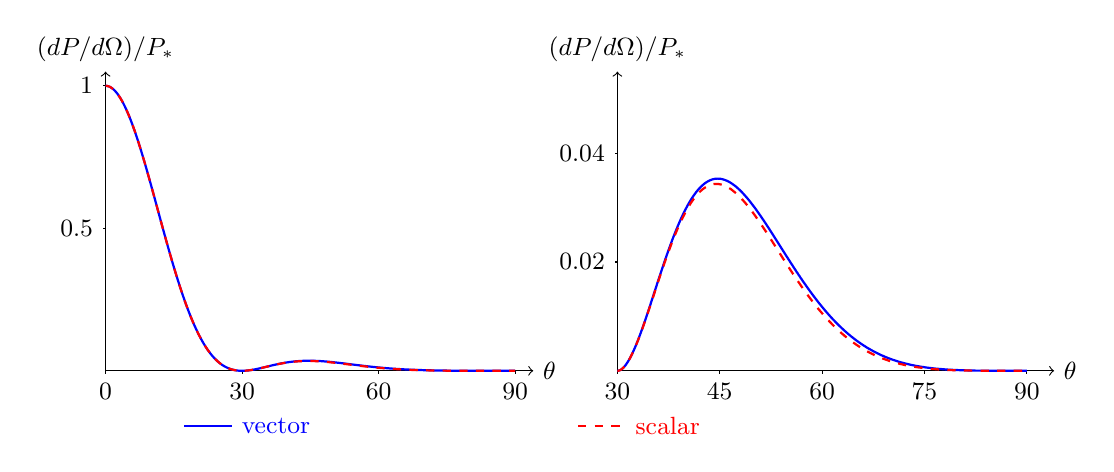
\begin{tikzpicture}[font=\small]
\begin{scope}[shift={(0cm,0)},x=0.05777777777777778cm,y=3.6190476190476186cm]
\begin{scope}[shift={(0,0)}]
\draw[->] (0,0) -- (94,0) node[right] {$\theta$};
\draw[->] (0,0) -- (0,1.05) node[above] {$(dP/d\Omega)/P_*$};
\draw (0,0) -- ++(0,-0.035cm) node[below] {$0$};
\draw (30,0) -- ++(0,-0.035cm) node[below] {$30$};
\draw (60,0) -- ++(0,-0.035cm) node[below] {$60$};
\draw (90,0) -- ++(0,-0.035cm) node[below] {$90$};
\draw (0,0.5) -- ++(-0.035cm,0) node[left] {$0.5$};
\draw (0,1) -- ++(-0.035cm,0) node[left] {$1$};
\draw[blue,thick] plot coordinates {(0.00000,1.000000) (0.15000,0.999906) (0.30000,0.999626) (0.45000,0.999158) (0.60000,0.998503) (0.75000,0.997662) (0.90000,0.996635) (1.05000,0.995422) (1.20000,0.994024) (1.35000,0.992441) (1.50000,0.990676) (1.65000,0.988727) (1.80000,0.986597) (1.95000,0.984286) (2.10000,0.981795) (2.25000,0.979126) (2.40000,0.976279) (2.55000,0.973257) (2.70000,0.970060) (2.85000,0.966691) (3.00000,0.963150) (3.15000,0.959440) (3.30000,0.955562) (3.45000,0.951518) (3.60000,0.947311) (3.75000,0.942941) (3.90000,0.938411) (4.05000,0.933723) (4.20000,0.928880) (4.35000,0.923883) (4.50000,0.918736) (4.65000,0.913440) (4.80000,0.907997) (4.95000,0.902412) (5.10000,0.896685) (5.25000,0.890820) (5.40000,0.884819) (5.55000,0.878685) (5.70000,0.872421) (5.85000,0.866030) (6.00000,0.859515) (6.15000,0.852878) (6.30000,0.846123) (6.45000,0.839253) (6.60000,0.832271) (6.75000,0.825179) (6.90000,0.817982) (7.05000,0.810682) (7.20000,0.803282) (7.35000,0.795786) (7.50000,0.788197) (7.65000,0.780519) (7.80000,0.772754) (7.95000,0.764906) (8.10000,0.756979) (8.25000,0.748975) (8.40000,0.740899) (8.55000,0.732754) (8.70000,0.724542) (8.85000,0.716268) (9.00000,0.707935) (9.15000,0.699546) (9.30000,0.691105) (9.45000,0.682616) (9.60000,0.674081) (9.75000,0.665504) (9.90000,0.656889) (10.05000,0.648239) (10.20000,0.639558) (10.35000,0.630849) (10.50000,0.622114) (10.65000,0.613359) (10.80000,0.604585) (10.95000,0.595797) (11.10000,0.586998) (11.25000,0.578191) (11.40000,0.569378) (11.55000,0.560565) (11.70000,0.551753) (11.85000,0.542946) (12.00000,0.534147) (12.15000,0.525359) (12.30000,0.516585) (12.45000,0.507829) (12.60000,0.499093) (12.75000,0.490380) (12.90000,0.481693) (13.05000,0.473035) (13.20000,0.464410) (13.35000,0.455818) (13.50000,0.447265) (13.65000,0.438751) (13.80000,0.430280) (13.95000,0.421854) (14.10000,0.413476) (14.25000,0.405149) (14.40000,0.396874) (14.55000,0.388654) (14.70000,0.380492) (14.85000,0.372390) (15.00000,0.364350) (15.15000,0.356373) (15.30000,0.348463) (15.45000,0.340621) (15.60000,0.332850) (15.75000,0.325150) (15.90000,0.317525) (16.05000,0.309975) (16.20000,0.302503) (16.35000,0.295110) (16.50000,0.287797) (16.65000,0.280567) (16.80000,0.273421) (16.95000,0.266360) (17.10000,0.259386) (17.25000,0.252500) (17.40000,0.245702) (17.55000,0.238996) (17.70000,0.232380) (17.85000,0.225857) (18.00000,0.219427) (18.15000,0.213092) (18.30000,0.206852) (18.45000,0.200708) (18.60000,0.194660) (18.75000,0.188711) (18.90000,0.182859) (19.05000,0.177105) (19.20000,0.171451) (19.35000,0.165897) (19.50000,0.160442) (19.65000,0.155087) (19.80000,0.149833) (19.95000,0.144680) (20.10000,0.139628) (20.25000,0.134676) (20.40000,0.129825) (20.55000,0.125076) (20.70000,0.120427) (20.85000,0.115879) (21.00000,0.111432) (21.15000,0.107085) (21.30000,0.102839) (21.45000,0.098692) (21.60000,0.094645) (21.75000,0.090696) (21.90000,0.086847) (22.05000,0.083095) (22.20000,0.079441) (22.35000,0.075884) (22.50000,0.072424) (22.65000,0.069059) (22.80000,0.065789) (22.95000,0.062613) (23.10000,0.059531) (23.25000,0.056542) (23.40000,0.053644) (23.55000,0.050838) (23.70000,0.048121) (23.85000,0.045494) (24.00000,0.042954) (24.15000,0.040502) (24.30000,0.038136) (24.45000,0.035855) (24.60000,0.033658) (24.75000,0.031543) (24.90000,0.029511) (25.05000,0.027559) (25.20000,0.025686) (25.35000,0.023892) (25.50000,0.022174) (25.65000,0.020533) (25.80000,0.018966) (25.95000,0.017472) (26.10000,0.016050) (26.25000,0.014699) (26.40000,0.013417) (26.55000,0.012204) (26.70000,0.011057) (26.85000,0.009976) (27.00000,0.008959) (27.15000,0.008004) (27.30000,0.007111) (27.45000,0.006278) (27.60000,0.005504) (27.75000,0.004787) (27.90000,0.004127) (28.05000,0.003521) (28.20000,0.002968) (28.35000,0.002467) (28.50000,0.002017) (28.65000,0.001616) (28.80000,0.001262) (28.95000,0.000956) (29.10000,0.000694) (29.25000,0.000477) (29.40000,0.000302) (29.55000,0.000168) (29.70000,0.000074) (29.85000,0.000018) (30.00000,0.000000) (30.15000,0.000018) (30.30000,0.000070) (30.45000,0.000156) (30.60000,0.000274) (30.75000,0.000423) (30.90000,0.000602) (31.05000,0.000809) (31.20000,0.001044) (31.35000,0.001305) (31.50000,0.001590) (31.65000,0.001900) (31.80000,0.002232) (31.95000,0.002586) (32.10000,0.002960) (32.25000,0.003353) (32.40000,0.003765) (32.55000,0.004193) (32.70000,0.004638) (32.85000,0.005099) (33.00000,0.005573) (33.15000,0.006060) (33.30000,0.006560) (33.45000,0.007071) (33.60000,0.007592) (33.75000,0.008122) (33.90000,0.008662) (34.05000,0.009208) (34.20000,0.009762) (34.35000,0.010322) (34.50000,0.010886) (34.65000,0.011455) (34.80000,0.012028) (34.95000,0.012604) (35.10000,0.013182) (35.25000,0.013761) (35.40000,0.014341) (35.55000,0.014921) (35.70000,0.015500) (35.85000,0.016079) (36.00000,0.016655) (36.15000,0.017229) (36.30000,0.017800) (36.45000,0.018368) (36.60000,0.018932) (36.75000,0.019491) (36.90000,0.020044) (37.05000,0.020593) (37.20000,0.021135) (37.35000,0.021671) (37.50000,0.022201) (37.65000,0.022723) (37.80000,0.023237) (37.95000,0.023744) (38.10000,0.024242) (38.25000,0.024731) (38.40000,0.025212) (38.55000,0.025683) (38.70000,0.026145) (38.85000,0.026596) (39.00000,0.027038) (39.15000,0.027470) (39.30000,0.027891) (39.45000,0.028301) (39.60000,0.028701) (39.75000,0.029089) (39.90000,0.029467) (40.05000,0.029832) (40.20000,0.030187) (40.35000,0.030530) (40.50000,0.030861) (40.65000,0.031180) (40.80000,0.031488) (40.95000,0.031783) (41.10000,0.032067) (41.25000,0.032338) (41.40000,0.032598) (41.55000,0.032845) (41.70000,0.033081) (41.85000,0.033304) (42.00000,0.033515) (42.15000,0.033714) (42.30000,0.033902) (42.45000,0.034077) (42.60000,0.034240) (42.75000,0.034391) (42.90000,0.034531) (43.05000,0.034659) (43.20000,0.034775) (43.35000,0.034880) (43.50000,0.034973) (43.65000,0.035055) (43.80000,0.035126) (43.95000,0.035185) (44.10000,0.035234) (44.25000,0.035272) (44.40000,0.035299) (44.55000,0.035315) (44.70000,0.035321) (44.85000,0.035316) (45.00000,0.035302) (45.15000,0.035277) (45.30000,0.035243) (45.45000,0.035199) (45.60000,0.035145) (45.75000,0.035082) (45.90000,0.035010) (46.05000,0.034929) (46.20000,0.034839) (46.35000,0.034740) (46.50000,0.034633) (46.65000,0.034518) (46.80000,0.034395) (46.95000,0.034263) (47.10000,0.034124) (47.25000,0.033978) (47.40000,0.033824) (47.55000,0.033663) (47.70000,0.033495) (47.85000,0.033321) (48.00000,0.033140) (48.15000,0.032952) (48.30000,0.032758) (48.45000,0.032559) (48.60000,0.032353) (48.75000,0.032142) (48.90000,0.031926) (49.05000,0.031704) (49.20000,0.031477) (49.35000,0.031246) (49.50000,0.031009) (49.65000,0.030769) (49.80000,0.030524) (49.95000,0.030275) (50.10000,0.030022) (50.25000,0.029765) (50.40000,0.029505) (50.55000,0.029241) (50.70000,0.028975) (50.85000,0.028705) (51.00000,0.028432) (51.15000,0.028157) (51.30000,0.027879) (51.45000,0.027598) (51.60000,0.027316) (51.75000,0.027031) (51.90000,0.026745) (52.05000,0.026457) (52.20000,0.026167) (52.35000,0.025876) (52.50000,0.025583) (52.65000,0.025289) (52.80000,0.024995) (52.95000,0.024699) (53.10000,0.024403) (53.25000,0.024106) (53.40000,0.023809) (53.55000,0.023511) (53.70000,0.023213) (53.85000,0.022915) (54.00000,0.022617) (54.15000,0.022319) (54.30000,0.022022) (54.45000,0.021724) (54.60000,0.021428) (54.75000,0.021131) (54.90000,0.020836) (55.05000,0.020541) (55.20000,0.020247) (55.35000,0.019954) (55.50000,0.019663) (55.65000,0.019372) (55.80000,0.019082) (55.95000,0.018794) (56.10000,0.018507) (56.25000,0.018222) (56.40000,0.017938) (56.55000,0.017656) (56.70000,0.017376) (56.85000,0.017097) (57.00000,0.016820) (57.15000,0.016545) (57.30000,0.016272) (57.45000,0.016001) (57.60000,0.015732) (57.75000,0.015465) (57.90000,0.015200) (58.05000,0.014938) (58.20000,0.014677) (58.35000,0.014419) (58.50000,0.014164) (58.65000,0.013910) (58.80000,0.013659) (58.95000,0.013411) (59.10000,0.013165) (59.25000,0.012921) (59.40000,0.012680) (59.55000,0.012442) (59.70000,0.012206) (59.85000,0.011973) (60.00000,0.011742) (60.15000,0.011514) (60.30000,0.011289) (60.45000,0.011066) (60.60000,0.010846) (60.75000,0.010629) (60.90000,0.010414) (61.05000,0.010203) (61.20000,0.009994) (61.35000,0.009787) (61.50000,0.009584) (61.65000,0.009383) (61.80000,0.009185) (61.95000,0.008989) (62.10000,0.008797) (62.25000,0.008607) (62.40000,0.008420) (62.55000,0.008235) (62.70000,0.008054) (62.85000,0.007875) (63.00000,0.007699) (63.15000,0.007525) (63.30000,0.007354) (63.45000,0.007186) (63.60000,0.007021) (63.75000,0.006858) (63.90000,0.006698) (64.05000,0.006540) (64.20000,0.006385) (64.35000,0.006233) (64.50000,0.006084) (64.65000,0.005936) (64.80000,0.005792) (64.95000,0.005650) (65.10000,0.005510) (65.25000,0.005373) (65.40000,0.005239) (65.55000,0.005107) (65.70000,0.004977) (65.85000,0.004850) (66.00000,0.004725) (66.15000,0.004603) (66.30000,0.004483) (66.45000,0.004365) (66.60000,0.004249) (66.75000,0.004136) (66.90000,0.004025) (67.05000,0.003917) (67.20000,0.003810) (67.35000,0.003706) (67.50000,0.003604) (67.65000,0.003503) (67.80000,0.003405) (67.95000,0.003310) (68.10000,0.003216) (68.25000,0.003124) (68.40000,0.003034) (68.55000,0.002946) (68.70000,0.002860) (68.85000,0.002776) (69.00000,0.002694) (69.15000,0.002614) (69.30000,0.002535) (69.45000,0.002458) (69.60000,0.002384) (69.75000,0.002310) (69.90000,0.002239) (70.05000,0.002169) (70.20000,0.002101) (70.35000,0.002035) (70.50000,0.001970) (70.65000,0.001907) (70.80000,0.001845) (70.95000,0.001785) (71.10000,0.001727) (71.25000,0.001669) (71.40000,0.001614) (71.55000,0.001560) (71.70000,0.001507) (71.85000,0.001455) (72.00000,0.001405) (72.15000,0.001357) (72.30000,0.001309) (72.45000,0.001263) (72.60000,0.001218) (72.75000,0.001175) (72.90000,0.001133) (73.05000,0.001091) (73.20000,0.001051) (73.35000,0.001012) (73.50000,0.000975) (73.65000,0.000938) (73.80000,0.000902) (73.95000,0.000868) (74.10000,0.000834) (74.25000,0.000802) (74.40000,0.000770) (74.55000,0.000740) (74.70000,0.000710) (74.85000,0.000682) (75.00000,0.000654) (75.15000,0.000627) (75.30000,0.000601) (75.45000,0.000576) (75.60000,0.000551) (75.75000,0.000528) (75.90000,0.000505) (76.05000,0.000483) (76.20000,0.000462) (76.35000,0.000441) (76.50000,0.000421) (76.65000,0.000402) (76.80000,0.000384) (76.95000,0.000366) (77.10000,0.000349) (77.25000,0.000332) (77.40000,0.000317) (77.55000,0.000301) (77.70000,0.000287) (77.85000,0.000272) (78.00000,0.000259) (78.15000,0.000246) (78.30000,0.000233) (78.45000,0.000221) (78.60000,0.000209) (78.75000,0.000198) (78.90000,0.000188) (79.05000,0.000177) (79.20000,0.000168) (79.35000,0.000158) (79.50000,0.000149) (79.65000,0.000141) (79.80000,0.000133) (79.95000,0.000125) (80.10000,0.000117) (80.25000,0.000110) (80.40000,0.000103) (80.55000,0.000097) (80.70000,0.000091) (80.85000,0.000085) (81.00000,0.000079) (81.15000,0.000074) (81.30000,0.000069) (81.45000,0.000064) (81.60000,0.000060) (81.75000,0.000056) (81.90000,0.000052) (82.05000,0.000048) (82.20000,0.000044) (82.35000,0.000041) (82.50000,0.000038) (82.65000,0.000035) (82.80000,0.000032) (82.95000,0.000029) (83.10000,0.000027) (83.25000,0.000025) (83.40000,0.000023) (83.55000,0.000021) (83.70000,0.000019) (83.85000,0.000017) (84.00000,0.000015) (84.15000,0.000014) (84.30000,0.000012) (84.45000,0.000011) (84.60000,0.000010) (84.75000,0.000009) (84.90000,0.000008) (85.05000,0.000007) (85.20000,0.000006) (85.35000,0.000005) (85.50000,0.000005) (85.65000,0.000004) (85.80000,0.000004) (85.95000,0.000003) (86.10000,0.000003) (86.25000,0.000002) (86.40000,0.000002) (86.55000,0.000002) (86.70000,0.000001) (86.85000,0.000001) (87.00000,0.000001) (87.15000,0.000001) (87.30000,0.000001) (87.45000,0.000000) (87.60000,0.000000) (87.75000,0.000000) (87.90000,0.000000) (88.05000,0.000000) (88.20000,0.000000) (88.35000,0.000000) (88.50000,0.000000) (88.65000,0.000000) (88.80000,0.000000) (88.95000,0.000000) (89.10000,0.000000) (89.25000,0.000000) (89.40000,0.000000) (89.55000,0.000000) (89.70000,0.000000) (89.85000,0.000000) (90.00000,0.000000)};
\draw[red,dashed,thick] plot coordinates {(0.00000,1.000000) (0.15000,0.999906) (0.30000,0.999626) (0.45000,0.999158) (0.60000,0.998503) (0.75000,0.997662) (0.90000,0.996635) (1.05000,0.995422) (1.20000,0.994024) (1.35000,0.992441) (1.50000,0.990676) (1.65000,0.988727) (1.80000,0.986597) (1.95000,0.984285) (2.10000,0.981795) (2.25000,0.979125) (2.40000,0.976279) (2.55000,0.973257) (2.70000,0.970060) (2.85000,0.966691) (3.00000,0.963150) (3.15000,0.959440) (3.30000,0.955562) (3.45000,0.951518) (3.60000,0.947310) (3.75000,0.942940) (3.90000,0.938410) (4.05000,0.933722) (4.20000,0.928878) (4.35000,0.923881) (4.50000,0.918734) (4.65000,0.913437) (4.80000,0.907995) (4.95000,0.902408) (5.10000,0.896681) (5.25000,0.890816) (5.40000,0.884814) (5.55000,0.878680) (5.70000,0.872416) (5.85000,0.866024) (6.00000,0.859509) (6.15000,0.852871) (6.30000,0.846116) (6.45000,0.839245) (6.60000,0.832262) (6.75000,0.825169) (6.90000,0.817971) (7.05000,0.810670) (7.20000,0.803270) (7.35000,0.795773) (7.50000,0.788183) (7.65000,0.780503) (7.80000,0.772737) (7.95000,0.764889) (8.10000,0.756960) (8.25000,0.748955) (8.40000,0.740878) (8.55000,0.732731) (8.70000,0.724518) (8.85000,0.716242) (9.00000,0.707908) (9.15000,0.699517) (9.30000,0.691075) (9.45000,0.682584) (9.60000,0.674047) (9.75000,0.665469) (9.90000,0.656852) (10.05000,0.648201) (10.20000,0.639517) (10.35000,0.630806) (10.50000,0.622070) (10.65000,0.613313) (10.80000,0.604537) (10.95000,0.595747) (11.10000,0.586946) (11.25000,0.578136) (11.40000,0.569322) (11.55000,0.560506) (11.70000,0.551692) (11.85000,0.542883) (12.00000,0.534082) (12.15000,0.525291) (12.30000,0.516516) (12.45000,0.507757) (12.60000,0.499019) (12.75000,0.490303) (12.90000,0.481614) (13.05000,0.472954) (13.20000,0.464326) (13.35000,0.455733) (13.50000,0.447177) (13.65000,0.438661) (13.80000,0.430188) (13.95000,0.421760) (14.10000,0.413380) (14.25000,0.405050) (14.40000,0.396773) (14.55000,0.388551) (14.70000,0.380387) (14.85000,0.372283) (15.00000,0.364240) (15.15000,0.356262) (15.30000,0.348350) (15.45000,0.340506) (15.60000,0.332733) (15.75000,0.325031) (15.90000,0.317404) (16.05000,0.309853) (16.20000,0.302379) (16.35000,0.294984) (16.50000,0.287670) (16.65000,0.280439) (16.80000,0.273291) (16.95000,0.266229) (17.10000,0.259254) (17.25000,0.252366) (17.40000,0.245568) (17.55000,0.238860) (17.70000,0.232243) (17.85000,0.225720) (18.00000,0.219289) (18.15000,0.212953) (18.30000,0.206713) (18.45000,0.200568) (18.60000,0.194521) (18.75000,0.188570) (18.90000,0.182718) (19.05000,0.176965) (19.20000,0.171311) (19.35000,0.165757) (19.50000,0.160302) (19.65000,0.154948) (19.80000,0.149694) (19.95000,0.144542) (20.10000,0.139490) (20.25000,0.134539) (20.40000,0.129690) (20.55000,0.124941) (20.70000,0.120293) (20.85000,0.115747) (21.00000,0.111301) (21.15000,0.106955) (21.30000,0.102710) (21.45000,0.098565) (21.60000,0.094519) (21.75000,0.090573) (21.90000,0.086725) (22.05000,0.082976) (22.20000,0.079324) (22.35000,0.075769) (22.50000,0.072311) (22.65000,0.068948) (22.80000,0.065680) (22.95000,0.062507) (23.10000,0.059428) (23.25000,0.056441) (23.40000,0.053546) (23.55000,0.050742) (23.70000,0.048028) (23.85000,0.045403) (24.00000,0.042867) (24.15000,0.040417) (24.30000,0.038054) (24.45000,0.035776) (24.60000,0.033582) (24.75000,0.031470) (24.90000,0.029441) (25.05000,0.027492) (25.20000,0.025622) (25.35000,0.023831) (25.50000,0.022117) (25.65000,0.020478) (25.80000,0.018914) (25.95000,0.017423) (26.10000,0.016004) (26.25000,0.014656) (26.40000,0.013377) (26.55000,0.012166) (26.70000,0.011022) (26.85000,0.009943) (27.00000,0.008929) (27.15000,0.007977) (27.30000,0.007087) (27.45000,0.006256) (27.60000,0.005484) (27.75000,0.004770) (27.90000,0.004111) (28.05000,0.003507) (28.20000,0.002956) (28.35000,0.002457) (28.50000,0.002008) (28.65000,0.001609) (28.80000,0.001257) (28.95000,0.000952) (29.10000,0.000691) (29.25000,0.000475) (29.40000,0.000300) (29.55000,0.000167) (29.70000,0.000073) (29.85000,0.000018) (30.00000,0.000000) (30.15000,0.000018) (30.30000,0.000070) (30.45000,0.000155) (30.60000,0.000273) (30.75000,0.000421) (30.90000,0.000599) (31.05000,0.000805) (31.20000,0.001038) (31.35000,0.001297) (31.50000,0.001580) (31.65000,0.001888) (31.80000,0.002217) (31.95000,0.002568) (32.10000,0.002939) (32.25000,0.003330) (32.40000,0.003738) (32.55000,0.004163) (32.70000,0.004604) (32.85000,0.005060) (33.00000,0.005530) (33.15000,0.006013) (33.30000,0.006508) (33.45000,0.007013) (33.60000,0.007529) (33.75000,0.008054) (33.90000,0.008587) (34.05000,0.009128) (34.20000,0.009675) (34.35000,0.010228) (34.50000,0.010786) (34.65000,0.011348) (34.80000,0.011913) (34.95000,0.012481) (35.10000,0.013051) (35.25000,0.013622) (35.40000,0.014194) (35.55000,0.014765) (35.70000,0.015335) (35.85000,0.015904) (36.00000,0.016472) (36.15000,0.017036) (36.30000,0.017597) (36.45000,0.018155) (36.60000,0.018708) (36.75000,0.019256) (36.90000,0.019799) (37.05000,0.020337) (37.20000,0.020868) (37.35000,0.021392) (37.50000,0.021910) (37.65000,0.022420) (37.80000,0.022922) (37.95000,0.023416) (38.10000,0.023902) (38.25000,0.024379) (38.40000,0.024846) (38.55000,0.025304) (38.70000,0.025753) (38.85000,0.026191) (39.00000,0.026620) (39.15000,0.027038) (39.30000,0.027445) (39.45000,0.027841) (39.60000,0.028227) (39.75000,0.028601) (39.90000,0.028964) (40.05000,0.029315) (40.20000,0.029655) (40.35000,0.029983) (40.50000,0.030300) (40.65000,0.030604) (40.80000,0.030897) (40.95000,0.031177) (41.10000,0.031446) (41.25000,0.031702) (41.40000,0.031947) (41.55000,0.032179) (41.70000,0.032399) (41.85000,0.032607) (42.00000,0.032803) (42.15000,0.032987) (42.30000,0.033159) (42.45000,0.033319) (42.60000,0.033467) (42.75000,0.033603) (42.90000,0.033727) (43.05000,0.033840) (43.20000,0.033941) (43.35000,0.034031) (43.50000,0.034109) (43.65000,0.034176) (43.80000,0.034232) (43.95000,0.034277) (44.10000,0.034311) (44.25000,0.034334) (44.40000,0.034346) (44.55000,0.034348) (44.70000,0.034340) (44.85000,0.034321) (45.00000,0.034292) (45.15000,0.034254) (45.30000,0.034206) (45.45000,0.034148) (45.60000,0.034081) (45.75000,0.034005) (45.90000,0.033920) (46.05000,0.033825) (46.20000,0.033723) (46.35000,0.033612) (46.50000,0.033492) (46.65000,0.033365) (46.80000,0.033229) (46.95000,0.033086) (47.10000,0.032936) (47.25000,0.032778) (47.40000,0.032613) (47.55000,0.032441) (47.70000,0.032263) (47.85000,0.032078) (48.00000,0.031887) (48.15000,0.031689) (48.30000,0.031486) (48.45000,0.031277) (48.60000,0.031062) (48.75000,0.030842) (48.90000,0.030617) (49.05000,0.030387) (49.20000,0.030152) (49.35000,0.029913) (49.50000,0.029669) (49.65000,0.029422) (49.80000,0.029170) (49.95000,0.028914) (50.10000,0.028655) (50.25000,0.028392) (50.40000,0.028126) (50.55000,0.027857) (50.70000,0.027585) (50.85000,0.027310) (51.00000,0.027033) (51.15000,0.026753) (51.30000,0.026471) (51.45000,0.026187) (51.60000,0.025901) (51.75000,0.025614) (51.90000,0.025324) (52.05000,0.025034) (52.20000,0.024742) (52.35000,0.024449) (52.50000,0.024155) (52.65000,0.023860) (52.80000,0.023564) (52.95000,0.023268) (53.10000,0.022971) (53.25000,0.022674) (53.40000,0.022377) (53.55000,0.022080) (53.70000,0.021783) (53.85000,0.021486) (54.00000,0.021189) (54.15000,0.020893) (54.30000,0.020597) (54.45000,0.020302) (54.60000,0.020008) (54.75000,0.019714) (54.90000,0.019422) (55.05000,0.019130) (55.20000,0.018840) (55.35000,0.018551) (55.50000,0.018263) (55.65000,0.017977) (55.80000,0.017692) (55.95000,0.017409) (56.10000,0.017127) (56.25000,0.016847) (56.40000,0.016569) (56.55000,0.016292) (56.70000,0.016018) (56.85000,0.015746) (57.00000,0.015475) (57.15000,0.015207) (57.30000,0.014941) (57.45000,0.014677) (57.60000,0.014415) (57.75000,0.014156) (57.90000,0.013899) (58.05000,0.013644) (58.20000,0.013392) (58.35000,0.013142) (58.50000,0.012895) (58.65000,0.012650) (58.80000,0.012408) (58.95000,0.012169) (59.10000,0.011932) (59.25000,0.011698) (59.40000,0.011466) (59.55000,0.011238) (59.70000,0.011012) (59.85000,0.010788) (60.00000,0.010568) (60.15000,0.010350) (60.30000,0.010135) (60.45000,0.009923) (60.60000,0.009714) (60.75000,0.009507) (60.90000,0.009303) (61.05000,0.009102) (61.20000,0.008904) (61.35000,0.008709) (61.50000,0.008517) (61.65000,0.008327) (61.80000,0.008140) (61.95000,0.007956) (62.10000,0.007775) (62.25000,0.007597) (62.40000,0.007421) (62.55000,0.007249) (62.70000,0.007079) (62.85000,0.006911) (63.00000,0.006747) (63.15000,0.006585) (63.30000,0.006426) (63.45000,0.006270) (63.60000,0.006117) (63.75000,0.005966) (63.90000,0.005818) (64.05000,0.005672) (64.20000,0.005529) (64.35000,0.005389) (64.50000,0.005251) (64.65000,0.005116) (64.80000,0.004984) (64.95000,0.004854) (65.10000,0.004726) (65.25000,0.004601) (65.40000,0.004478) (65.55000,0.004358) (65.70000,0.004240) (65.85000,0.004125) (66.00000,0.004012) (66.15000,0.003901) (66.30000,0.003793) (66.45000,0.003686) (66.60000,0.003582) (66.75000,0.003481) (66.90000,0.003381) (67.05000,0.003284) (67.20000,0.003189) (67.35000,0.003096) (67.50000,0.003005) (67.65000,0.002916) (67.80000,0.002829) (67.95000,0.002744) (68.10000,0.002661) (68.25000,0.002580) (68.40000,0.002501) (68.55000,0.002423) (68.70000,0.002348) (68.85000,0.002274) (69.00000,0.002202) (69.15000,0.002132) (69.30000,0.002064) (69.45000,0.001997) (69.60000,0.001933) (69.75000,0.001869) (69.90000,0.001808) (70.05000,0.001748) (70.20000,0.001689) (70.35000,0.001632) (70.50000,0.001577) (70.65000,0.001523) (70.80000,0.001470) (70.95000,0.001419) (71.10000,0.001369) (71.25000,0.001321) (71.40000,0.001274) (71.55000,0.001228) (71.70000,0.001184) (71.85000,0.001141) (72.00000,0.001099) (72.15000,0.001059) (72.30000,0.001019) (72.45000,0.000981) (72.60000,0.000944) (72.75000,0.000908) (72.90000,0.000873) (73.05000,0.000839) (73.20000,0.000806) (73.35000,0.000774) (73.50000,0.000743) (73.65000,0.000714) (73.80000,0.000685) (73.95000,0.000657) (74.10000,0.000630) (74.25000,0.000604) (74.40000,0.000578) (74.55000,0.000554) (74.70000,0.000530) (74.85000,0.000508) (75.00000,0.000485) (75.15000,0.000464) (75.30000,0.000444) (75.45000,0.000424) (75.60000,0.000405) (75.75000,0.000386) (75.90000,0.000369) (76.05000,0.000352) (76.20000,0.000335) (76.35000,0.000319) (76.50000,0.000304) (76.65000,0.000289) (76.80000,0.000275) (76.95000,0.000262) (77.10000,0.000249) (77.25000,0.000236) (77.40000,0.000224) (77.55000,0.000213) (77.70000,0.000202) (77.85000,0.000191) (78.00000,0.000181) (78.15000,0.000171) (78.30000,0.000162) (78.45000,0.000153) (78.60000,0.000145) (78.75000,0.000136) (78.90000,0.000129) (79.05000,0.000121) (79.20000,0.000114) (79.35000,0.000107) (79.50000,0.000101) (79.65000,0.000095) (79.80000,0.000089) (79.95000,0.000083) (80.10000,0.000078) (80.25000,0.000073) (80.40000,0.000068) (80.55000,0.000064) (80.70000,0.000060) (80.85000,0.000056) (81.00000,0.000052) (81.15000,0.000048) (81.30000,0.000045) (81.45000,0.000042) (81.60000,0.000039) (81.75000,0.000036) (81.90000,0.000033) (82.05000,0.000030) (82.20000,0.000028) (82.35000,0.000026) (82.50000,0.000024) (82.65000,0.000022) (82.80000,0.000020) (82.95000,0.000018) (83.10000,0.000017) (83.25000,0.000015) (83.40000,0.000014) (83.55000,0.000013) (83.70000,0.000011) (83.85000,0.000010) (84.00000,0.000009) (84.15000,0.000008) (84.30000,0.000007) (84.45000,0.000007) (84.60000,0.000006) (84.75000,0.000005) (84.90000,0.000005) (85.05000,0.000004) (85.20000,0.000004) (85.35000,0.000003) (85.50000,0.000003) (85.65000,0.000002) (85.80000,0.000002) (85.95000,0.000002) (86.10000,0.000002) (86.25000,0.000001) (86.40000,0.000001) (86.55000,0.000001) (86.70000,0.000001) (86.85000,0.000001) (87.00000,0.000001) (87.15000,0.000000) (87.30000,0.000000) (87.45000,0.000000) (87.60000,0.000000) (87.75000,0.000000) (87.90000,0.000000) (88.05000,0.000000) (88.20000,0.000000) (88.35000,0.000000) (88.50000,0.000000) (88.65000,0.000000) (88.80000,0.000000) (88.95000,0.000000) (89.10000,0.000000) (89.25000,0.000000) (89.40000,0.000000) (89.55000,0.000000) (89.70000,0.000000) (89.85000,0.000000) (90.00000,0.000000)};
\end{scope}\end{scope}
\begin{scope}[shift={(6.5cm,0)},x=0.08666666666666667cm,y=69.0909090909091cm]
\begin{scope}[shift={(-30,0)}]
\draw[->] (30,0) -- (94,0) node[right] {$\theta$};
\draw[->] (30,0) -- (30,0.055) node[above] {$(dP/d\Omega)/P_*$};
\draw (30,0) -- ++(0,-0.035cm) node[below] {$30$};
\draw (45,0) -- ++(0,-0.035cm) node[below] {$45$};
\draw (60,0) -- ++(0,-0.035cm) node[below] {$60$};
\draw (75,0) -- ++(0,-0.035cm) node[below] {$75$};
\draw (90,0) -- ++(0,-0.035cm) node[below] {$90$};
\draw (30,0.02) -- ++(-0.035cm,0) node[left] {$0.02$};
\draw (30,0.04) -- ++(-0.035cm,0) node[left] {$0.04$};
\draw[blue,thick] plot coordinates {(30.00000,0.000000) (30.15000,0.000018) (30.30000,0.000070) (30.45000,0.000156) (30.60000,0.000274) (30.75000,0.000423) (30.90000,0.000602) (31.05000,0.000809) (31.20000,0.001044) (31.35000,0.001305) (31.50000,0.001590) (31.65000,0.001900) (31.80000,0.002232) (31.95000,0.002586) (32.10000,0.002960) (32.25000,0.003353) (32.40000,0.003765) (32.55000,0.004193) (32.70000,0.004638) (32.85000,0.005099) (33.00000,0.005573) (33.15000,0.006060) (33.30000,0.006560) (33.45000,0.007071) (33.60000,0.007592) (33.75000,0.008122) (33.90000,0.008662) (34.05000,0.009208) (34.20000,0.009762) (34.35000,0.010322) (34.50000,0.010886) (34.65000,0.011455) (34.80000,0.012028) (34.95000,0.012604) (35.10000,0.013182) (35.25000,0.013761) (35.40000,0.014341) (35.55000,0.014921) (35.70000,0.015500) (35.85000,0.016079) (36.00000,0.016655) (36.15000,0.017229) (36.30000,0.017800) (36.45000,0.018368) (36.60000,0.018932) (36.75000,0.019491) (36.90000,0.020044) (37.05000,0.020593) (37.20000,0.021135) (37.35000,0.021671) (37.50000,0.022201) (37.65000,0.022723) (37.80000,0.023237) (37.95000,0.023744) (38.10000,0.024242) (38.25000,0.024731) (38.40000,0.025212) (38.55000,0.025683) (38.70000,0.026145) (38.85000,0.026596) (39.00000,0.027038) (39.15000,0.027470) (39.30000,0.027891) (39.45000,0.028301) (39.60000,0.028701) (39.75000,0.029089) (39.90000,0.029467) (40.05000,0.029832) (40.20000,0.030187) (40.35000,0.030530) (40.50000,0.030861) (40.65000,0.031180) (40.80000,0.031488) (40.95000,0.031783) (41.10000,0.032067) (41.25000,0.032338) (41.40000,0.032598) (41.55000,0.032845) (41.70000,0.033081) (41.85000,0.033304) (42.00000,0.033515) (42.15000,0.033714) (42.30000,0.033902) (42.45000,0.034077) (42.60000,0.034240) (42.75000,0.034391) (42.90000,0.034531) (43.05000,0.034659) (43.20000,0.034775) (43.35000,0.034880) (43.50000,0.034973) (43.65000,0.035055) (43.80000,0.035126) (43.95000,0.035185) (44.10000,0.035234) (44.25000,0.035272) (44.40000,0.035299) (44.55000,0.035315) (44.70000,0.035321) (44.85000,0.035316) (45.00000,0.035302) (45.15000,0.035277) (45.30000,0.035243) (45.45000,0.035199) (45.60000,0.035145) (45.75000,0.035082) (45.90000,0.035010) (46.05000,0.034929) (46.20000,0.034839) (46.35000,0.034740) (46.50000,0.034633) (46.65000,0.034518) (46.80000,0.034395) (46.95000,0.034263) (47.10000,0.034124) (47.25000,0.033978) (47.40000,0.033824) (47.55000,0.033663) (47.70000,0.033495) (47.85000,0.033321) (48.00000,0.033140) (48.15000,0.032952) (48.30000,0.032758) (48.45000,0.032559) (48.60000,0.032353) (48.75000,0.032142) (48.90000,0.031926) (49.05000,0.031704) (49.20000,0.031477) (49.35000,0.031246) (49.50000,0.031009) (49.65000,0.030769) (49.80000,0.030524) (49.95000,0.030275) (50.10000,0.030022) (50.25000,0.029765) (50.40000,0.029505) (50.55000,0.029241) (50.70000,0.028975) (50.85000,0.028705) (51.00000,0.028432) (51.15000,0.028157) (51.30000,0.027879) (51.45000,0.027598) (51.60000,0.027316) (51.75000,0.027031) (51.90000,0.026745) (52.05000,0.026457) (52.20000,0.026167) (52.35000,0.025876) (52.50000,0.025583) (52.65000,0.025289) (52.80000,0.024995) (52.95000,0.024699) (53.10000,0.024403) (53.25000,0.024106) (53.40000,0.023809) (53.55000,0.023511) (53.70000,0.023213) (53.85000,0.022915) (54.00000,0.022617) (54.15000,0.022319) (54.30000,0.022022) (54.45000,0.021724) (54.60000,0.021428) (54.75000,0.021131) (54.90000,0.020836) (55.05000,0.020541) (55.20000,0.020247) (55.35000,0.019954) (55.50000,0.019663) (55.65000,0.019372) (55.80000,0.019082) (55.95000,0.018794) (56.10000,0.018507) (56.25000,0.018222) (56.40000,0.017938) (56.55000,0.017656) (56.70000,0.017376) (56.85000,0.017097) (57.00000,0.016820) (57.15000,0.016545) (57.30000,0.016272) (57.45000,0.016001) (57.60000,0.015732) (57.75000,0.015465) (57.90000,0.015200) (58.05000,0.014938) (58.20000,0.014677) (58.35000,0.014419) (58.50000,0.014164) (58.65000,0.013910) (58.80000,0.013659) (58.95000,0.013411) (59.10000,0.013165) (59.25000,0.012921) (59.40000,0.012680) (59.55000,0.012442) (59.70000,0.012206) (59.85000,0.011973) (60.00000,0.011742) (60.15000,0.011514) (60.30000,0.011289) (60.45000,0.011066) (60.60000,0.010846) (60.75000,0.010629) (60.90000,0.010414) (61.05000,0.010203) (61.20000,0.009994) (61.35000,0.009787) (61.50000,0.009584) (61.65000,0.009383) (61.80000,0.009185) (61.95000,0.008989) (62.10000,0.008797) (62.25000,0.008607) (62.40000,0.008420) (62.55000,0.008235) (62.70000,0.008054) (62.85000,0.007875) (63.00000,0.007699) (63.15000,0.007525) (63.30000,0.007354) (63.45000,0.007186) (63.60000,0.007021) (63.75000,0.006858) (63.90000,0.006698) (64.05000,0.006540) (64.20000,0.006385) (64.35000,0.006233) (64.50000,0.006084) (64.65000,0.005936) (64.80000,0.005792) (64.95000,0.005650) (65.10000,0.005510) (65.25000,0.005373) (65.40000,0.005239) (65.55000,0.005107) (65.70000,0.004977) (65.85000,0.004850) (66.00000,0.004725) (66.15000,0.004603) (66.30000,0.004483) (66.45000,0.004365) (66.60000,0.004249) (66.75000,0.004136) (66.90000,0.004025) (67.05000,0.003917) (67.20000,0.003810) (67.35000,0.003706) (67.50000,0.003604) (67.65000,0.003503) (67.80000,0.003405) (67.95000,0.003310) (68.10000,0.003216) (68.25000,0.003124) (68.40000,0.003034) (68.55000,0.002946) (68.70000,0.002860) (68.85000,0.002776) (69.00000,0.002694) (69.15000,0.002614) (69.30000,0.002535) (69.45000,0.002458) (69.60000,0.002384) (69.75000,0.002310) (69.90000,0.002239) (70.05000,0.002169) (70.20000,0.002101) (70.35000,0.002035) (70.50000,0.001970) (70.65000,0.001907) (70.80000,0.001845) (70.95000,0.001785) (71.10000,0.001727) (71.25000,0.001669) (71.40000,0.001614) (71.55000,0.001560) (71.70000,0.001507) (71.85000,0.001455) (72.00000,0.001405) (72.15000,0.001357) (72.30000,0.001309) (72.45000,0.001263) (72.60000,0.001218) (72.75000,0.001175) (72.90000,0.001133) (73.05000,0.001091) (73.20000,0.001051) (73.35000,0.001012) (73.50000,0.000975) (73.65000,0.000938) (73.80000,0.000902) (73.95000,0.000868) (74.10000,0.000834) (74.25000,0.000802) (74.40000,0.000770) (74.55000,0.000740) (74.70000,0.000710) (74.85000,0.000682) (75.00000,0.000654) (75.15000,0.000627) (75.30000,0.000601) (75.45000,0.000576) (75.60000,0.000551) (75.75000,0.000528) (75.90000,0.000505) (76.05000,0.000483) (76.20000,0.000462) (76.35000,0.000441) (76.50000,0.000421) (76.65000,0.000402) (76.80000,0.000384) (76.95000,0.000366) (77.10000,0.000349) (77.25000,0.000332) (77.40000,0.000317) (77.55000,0.000301) (77.70000,0.000287) (77.85000,0.000272) (78.00000,0.000259) (78.15000,0.000246) (78.30000,0.000233) (78.45000,0.000221) (78.60000,0.000209) (78.75000,0.000198) (78.90000,0.000188) (79.05000,0.000177) (79.20000,0.000168) (79.35000,0.000158) (79.50000,0.000149) (79.65000,0.000141) (79.80000,0.000133) (79.95000,0.000125) (80.10000,0.000117) (80.25000,0.000110) (80.40000,0.000103) (80.55000,0.000097) (80.70000,0.000091) (80.85000,0.000085) (81.00000,0.000079) (81.15000,0.000074) (81.30000,0.000069) (81.45000,0.000064) (81.60000,0.000060) (81.75000,0.000056) (81.90000,0.000052) (82.05000,0.000048) (82.20000,0.000044) (82.35000,0.000041) (82.50000,0.000038) (82.65000,0.000035) (82.80000,0.000032) (82.95000,0.000029) (83.10000,0.000027) (83.25000,0.000025) (83.40000,0.000023) (83.55000,0.000021) (83.70000,0.000019) (83.85000,0.000017) (84.00000,0.000015) (84.15000,0.000014) (84.30000,0.000012) (84.45000,0.000011) (84.60000,0.000010) (84.75000,0.000009) (84.90000,0.000008) (85.05000,0.000007) (85.20000,0.000006) (85.35000,0.000005) (85.50000,0.000005) (85.65000,0.000004) (85.80000,0.000004) (85.95000,0.000003) (86.10000,0.000003) (86.25000,0.000002) (86.40000,0.000002) (86.55000,0.000002) (86.70000,0.000001) (86.85000,0.000001) (87.00000,0.000001) (87.15000,0.000001) (87.30000,0.000001) (87.45000,0.000000) (87.60000,0.000000) (87.75000,0.000000) (87.90000,0.000000) (88.05000,0.000000) (88.20000,0.000000) (88.35000,0.000000) (88.50000,0.000000) (88.65000,0.000000) (88.80000,0.000000) (88.95000,0.000000) (89.10000,0.000000) (89.25000,0.000000) (89.40000,0.000000) (89.55000,0.000000) (89.70000,0.000000) (89.85000,0.000000) (90.00000,0.000000)};
\draw[red,dashed,thick] plot coordinates {(30.00000,0.000000) (30.15000,0.000018) (30.30000,0.000070) (30.45000,0.000155) (30.60000,0.000273) (30.75000,0.000421) (30.90000,0.000599) (31.05000,0.000805) (31.20000,0.001038) (31.35000,0.001297) (31.50000,0.001580) (31.65000,0.001888) (31.80000,0.002217) (31.95000,0.002568) (32.10000,0.002939) (32.25000,0.003330) (32.40000,0.003738) (32.55000,0.004163) (32.70000,0.004604) (32.85000,0.005060) (33.00000,0.005530) (33.15000,0.006013) (33.30000,0.006508) (33.45000,0.007013) (33.60000,0.007529) (33.75000,0.008054) (33.90000,0.008587) (34.05000,0.009128) (34.20000,0.009675) (34.35000,0.010228) (34.50000,0.010786) (34.65000,0.011348) (34.80000,0.011913) (34.95000,0.012481) (35.10000,0.013051) (35.25000,0.013622) (35.40000,0.014194) (35.55000,0.014765) (35.70000,0.015335) (35.85000,0.015904) (36.00000,0.016472) (36.15000,0.017036) (36.30000,0.017597) (36.45000,0.018155) (36.60000,0.018708) (36.75000,0.019256) (36.90000,0.019799) (37.05000,0.020337) (37.20000,0.020868) (37.35000,0.021392) (37.50000,0.021910) (37.65000,0.022420) (37.80000,0.022922) (37.95000,0.023416) (38.10000,0.023902) (38.25000,0.024379) (38.40000,0.024846) (38.55000,0.025304) (38.70000,0.025753) (38.85000,0.026191) (39.00000,0.026620) (39.15000,0.027038) (39.30000,0.027445) (39.45000,0.027841) (39.60000,0.028227) (39.75000,0.028601) (39.90000,0.028964) (40.05000,0.029315) (40.20000,0.029655) (40.35000,0.029983) (40.50000,0.030300) (40.65000,0.030604) (40.80000,0.030897) (40.95000,0.031177) (41.10000,0.031446) (41.25000,0.031702) (41.40000,0.031947) (41.55000,0.032179) (41.70000,0.032399) (41.85000,0.032607) (42.00000,0.032803) (42.15000,0.032987) (42.30000,0.033159) (42.45000,0.033319) (42.60000,0.033467) (42.75000,0.033603) (42.90000,0.033727) (43.05000,0.033840) (43.20000,0.033941) (43.35000,0.034031) (43.50000,0.034109) (43.65000,0.034176) (43.80000,0.034232) (43.95000,0.034277) (44.10000,0.034311) (44.25000,0.034334) (44.40000,0.034346) (44.55000,0.034348) (44.70000,0.034340) (44.85000,0.034321) (45.00000,0.034292) (45.15000,0.034254) (45.30000,0.034206) (45.45000,0.034148) (45.60000,0.034081) (45.75000,0.034005) (45.90000,0.033920) (46.05000,0.033825) (46.20000,0.033723) (46.35000,0.033612) (46.50000,0.033492) (46.65000,0.033365) (46.80000,0.033229) (46.95000,0.033086) (47.10000,0.032936) (47.25000,0.032778) (47.40000,0.032613) (47.55000,0.032441) (47.70000,0.032263) (47.85000,0.032078) (48.00000,0.031887) (48.15000,0.031689) (48.30000,0.031486) (48.45000,0.031277) (48.60000,0.031062) (48.75000,0.030842) (48.90000,0.030617) (49.05000,0.030387) (49.20000,0.030152) (49.35000,0.029913) (49.50000,0.029669) (49.65000,0.029422) (49.80000,0.029170) (49.95000,0.028914) (50.10000,0.028655) (50.25000,0.028392) (50.40000,0.028126) (50.55000,0.027857) (50.70000,0.027585) (50.85000,0.027310) (51.00000,0.027033) (51.15000,0.026753) (51.30000,0.026471) (51.45000,0.026187) (51.60000,0.025901) (51.75000,0.025614) (51.90000,0.025324) (52.05000,0.025034) (52.20000,0.024742) (52.35000,0.024449) (52.50000,0.024155) (52.65000,0.023860) (52.80000,0.023564) (52.95000,0.023268) (53.10000,0.022971) (53.25000,0.022674) (53.40000,0.022377) (53.55000,0.022080) (53.70000,0.021783) (53.85000,0.021486) (54.00000,0.021189) (54.15000,0.020893) (54.30000,0.020597) (54.45000,0.020302) (54.60000,0.020008) (54.75000,0.019714) (54.90000,0.019422) (55.05000,0.019130) (55.20000,0.018840) (55.35000,0.018551) (55.50000,0.018263) (55.65000,0.017977) (55.80000,0.017692) (55.95000,0.017409) (56.10000,0.017127) (56.25000,0.016847) (56.40000,0.016569) (56.55000,0.016292) (56.70000,0.016018) (56.85000,0.015746) (57.00000,0.015475) (57.15000,0.015207) (57.30000,0.014941) (57.45000,0.014677) (57.60000,0.014415) (57.75000,0.014156) (57.90000,0.013899) (58.05000,0.013644) (58.20000,0.013392) (58.35000,0.013142) (58.50000,0.012895) (58.65000,0.012650) (58.80000,0.012408) (58.95000,0.012169) (59.10000,0.011932) (59.25000,0.011698) (59.40000,0.011466) (59.55000,0.011238) (59.70000,0.011012) (59.85000,0.010788) (60.00000,0.010568) (60.15000,0.010350) (60.30000,0.010135) (60.45000,0.009923) (60.60000,0.009714) (60.75000,0.009507) (60.90000,0.009303) (61.05000,0.009102) (61.20000,0.008904) (61.35000,0.008709) (61.50000,0.008517) (61.65000,0.008327) (61.80000,0.008140) (61.95000,0.007956) (62.10000,0.007775) (62.25000,0.007597) (62.40000,0.007421) (62.55000,0.007249) (62.70000,0.007079) (62.85000,0.006911) (63.00000,0.006747) (63.15000,0.006585) (63.30000,0.006426) (63.45000,0.006270) (63.60000,0.006117) (63.75000,0.005966) (63.90000,0.005818) (64.05000,0.005672) (64.20000,0.005529) (64.35000,0.005389) (64.50000,0.005251) (64.65000,0.005116) (64.80000,0.004984) (64.95000,0.004854) (65.10000,0.004726) (65.25000,0.004601) (65.40000,0.004478) (65.55000,0.004358) (65.70000,0.004240) (65.85000,0.004125) (66.00000,0.004012) (66.15000,0.003901) (66.30000,0.003793) (66.45000,0.003686) (66.60000,0.003582) (66.75000,0.003481) (66.90000,0.003381) (67.05000,0.003284) (67.20000,0.003189) (67.35000,0.003096) (67.50000,0.003005) (67.65000,0.002916) (67.80000,0.002829) (67.95000,0.002744) (68.10000,0.002661) (68.25000,0.002580) (68.40000,0.002501) (68.55000,0.002423) (68.70000,0.002348) (68.85000,0.002274) (69.00000,0.002202) (69.15000,0.002132) (69.30000,0.002064) (69.45000,0.001997) (69.60000,0.001933) (69.75000,0.001869) (69.90000,0.001808) (70.05000,0.001748) (70.20000,0.001689) (70.35000,0.001632) (70.50000,0.001577) (70.65000,0.001523) (70.80000,0.001470) (70.95000,0.001419) (71.10000,0.001369) (71.25000,0.001321) (71.40000,0.001274) (71.55000,0.001228) (71.70000,0.001184) (71.85000,0.001141) (72.00000,0.001099) (72.15000,0.001059) (72.30000,0.001019) (72.45000,0.000981) (72.60000,0.000944) (72.75000,0.000908) (72.90000,0.000873) (73.05000,0.000839) (73.20000,0.000806) (73.35000,0.000774) (73.50000,0.000743) (73.65000,0.000714) (73.80000,0.000685) (73.95000,0.000657) (74.10000,0.000630) (74.25000,0.000604) (74.40000,0.000578) (74.55000,0.000554) (74.70000,0.000530) (74.85000,0.000508) (75.00000,0.000485) (75.15000,0.000464) (75.30000,0.000444) (75.45000,0.000424) (75.60000,0.000405) (75.75000,0.000386) (75.90000,0.000369) (76.05000,0.000352) (76.20000,0.000335) (76.35000,0.000319) (76.50000,0.000304) (76.65000,0.000289) (76.80000,0.000275) (76.95000,0.000262) (77.10000,0.000249) (77.25000,0.000236) (77.40000,0.000224) (77.55000,0.000213) (77.70000,0.000202) (77.85000,0.000191) (78.00000,0.000181) (78.15000,0.000171) (78.30000,0.000162) (78.45000,0.000153) (78.60000,0.000145) (78.75000,0.000136) (78.90000,0.000129) (79.05000,0.000121) (79.20000,0.000114) (79.35000,0.000107) (79.50000,0.000101) (79.65000,0.000095) (79.80000,0.000089) (79.95000,0.000083) (80.10000,0.000078) (80.25000,0.000073) (80.40000,0.000068) (80.55000,0.000064) (80.70000,0.000060) (80.85000,0.000056) (81.00000,0.000052) (81.15000,0.000048) (81.30000,0.000045) (81.45000,0.000042) (81.60000,0.000039) (81.75000,0.000036) (81.90000,0.000033) (82.05000,0.000030) (82.20000,0.000028) (82.35000,0.000026) (82.50000,0.000024) (82.65000,0.000022) (82.80000,0.000020) (82.95000,0.000018) (83.10000,0.000017) (83.25000,0.000015) (83.40000,0.000014) (83.55000,0.000013) (83.70000,0.000011) (83.85000,0.000010) (84.00000,0.000009) (84.15000,0.000008) (84.30000,0.000007) (84.45000,0.000007) (84.60000,0.000006) (84.75000,0.000005) (84.90000,0.000005) (85.05000,0.000004) (85.20000,0.000004) (85.35000,0.000003) (85.50000,0.000003) (85.65000,0.000002) (85.80000,0.000002) (85.95000,0.000002) (86.10000,0.000002) (86.25000,0.000001) (86.40000,0.000001) (86.55000,0.000001) (86.70000,0.000001) (86.85000,0.000001) (87.00000,0.000001) (87.15000,0.000000) (87.30000,0.000000) (87.45000,0.000000) (87.60000,0.000000) (87.75000,0.000000) (87.90000,0.000000) (88.05000,0.000000) (88.20000,0.000000) (88.35000,0.000000) (88.50000,0.000000) (88.65000,0.000000) (88.80000,0.000000) (88.95000,0.000000) (89.10000,0.000000) (89.25000,0.000000) (89.40000,0.000000) (89.55000,0.000000) (89.70000,0.000000) (89.85000,0.000000) (90.00000,0.000000)};
\end{scope}\end{scope}
\draw[blue,thick] (1cm,-.7cm)--(1.6cm,-.7cm) node[right] {vector};
\draw[red,dashed,thick] (6cm,-.7cm)--(6.6cm,-.7cm) node[right] {scalar};
\end{tikzpicture}
\end{center}

\Needspace{5\baselineskip}
\par\bigskip
\noindent\textbf{10.15}\quad A cylindrical coaxial transmission line of inner radius $a$ and outer radius $b$ has its axis along the negative $z$ axis. Both inner and outer conductors end at $z=0$, and the outer one is connected to an infinite plane copper flange occupying the whole $x$-$y$ plane (except for the annulus of inner radius $a$ and outer radius $b$ around the origin). The transmission line is excited at frequency $\omega$ in its dominant TEM mode, with the peak voltage between the cylinders being $V$. Use the vector Smythe--Kirchhoff approximation to discuss the radiated fields, the angular distribution of radiation, and the total power radiated.
\solution
Assume vacuum in the coax and neglect the finite surface resistance of
the copper flange. The prescribed Smythe--Kirchhoff approximation uses
the unperturbed TEM aperture field
\[
\mathbf E_t(\rho,0)=\frac{V}{\rho\ln(b/a)}\widehat{\boldsymbol\rho},
\qquad a<\rho<b.
\]
Here $V$ is a \emph{peak phasor voltage}; time-averaged powers contain
$1/2$. Put $\ell=\ln(b/a)$ and $q=k\sin\theta$. Choosing the observation
azimuth as zero during the integral,
\[
\begin{split}
\int_A\widehat{\mathbf z}\times\mathbf E_t\,
e^{-i\mathbf k_t\cdot\mathbf r'}da'
&=\frac{V}{\ell}\int_a^b d\rho\int_0^{2\pi}
\widehat{\boldsymbol\varphi}'e^{-iq\rho\cos\varphi'}d\varphi'\\
&=-\frac{2\pi iV}{q\ell}[J_0(qa)-J_0(qb)]
\widehat{\boldsymbol\varphi}.
\end{split}
\]
Since $\mathbf n\times\widehat{\boldsymbol\varphi}
=-\widehat{\boldsymbol\theta}$, the radiation fields are
\[
\boxed{E_\theta=-\frac{Ve^{ikr-i\omega t}}{r\ell}
\frac{J_0(ka\sin\theta)-J_0(kb\sin\theta)}{\sin\theta},
\qquad B_\varphi=E_\theta/c.}
\]
All other leading $1/r$ components vanish. The apparent axial singularity
is removable: the numerator is
$k^2(b^2-a^2)\sin^2\theta/4+O(\sin^4\theta)$, so $E_\theta=0$ on axis.
The polarization is meridional and the intensity is azimuthally symmetric:
\[
\boxed{\frac{dP}{d\Omega}=\frac{|V|^2}{2Z_0\ell^2}
\frac{[J_0(ka\sin\theta)-J_0(kb\sin\theta)]^2}{\sin^2\theta}.}
\]
Only the upper hemisphere is radiated into, giving the convergent
one-dimensional formula, valid at arbitrary $ka,kb$ within this model,
\[
\boxed{P=\frac{\pi|V|^2}{Z_0\ell^2}
\int_0^{\pi/2}
\frac{[J_0(ka\sin\theta)-J_0(kb\sin\theta)]^2}{\sin\theta}\,d\theta.}
\]
For $kb\ll1$,
\[
P\simeq\frac{\pi|V|^2 k^4(b^2-a^2)^2}{24Z_0\ell^2},
\qquad
\frac{dP}{d\Omega}\simeq
\frac{|V|^2 k^4(b^2-a^2)^2}{32Z_0\ell^2}\sin^2\theta .
\]
This is the pattern of a normal electric dipole; the zeroth aperture
magnetic moment vanishes by rotational symmetry.

The incident TEM power for the same voltage is
$P_{\rm TEM}=|V|^2/(2Z_c)=\pi|V|^2/(Z_0\ell)$, with
$Z_c=Z_0\ell/(2\pi)$. Thus the displayed integral divided by $\ell$ is
the approximate transmission fraction. At large $ka,kb$ with fixed
$b/a$, set $u=k\sin\theta$ in its forward-dominated contribution and use
\[
\int_0^\infty[J_0(au)-J_0(bu)]^2\,\frac{du}{u}=\ln(b/a)
\]
to obtain $P/P_{\rm TEM}\to1$. To verify this last integral, call its
left side $I(a,b)$. Hankel inversion of a disk indicator gives
$\int_0^\infty J_0(au)J_1(bu)\,du=1/b$ for $a<b$, while
$\int_0^\infty J_0(bu)J_1(bu)\,du=1/(2b)$ follows by integrating
$-(2b)^{-1}\,d[J_0(bu)^2]/du$. Therefore
\[
\partial_b I=2\int_0^\infty[J_0(au)-J_0(bu)]J_1(bu)\,du
=\frac1b,\qquad I(a,a)=0,
\]
which proves $I=\ln(b/a)$ (oscillatory integrals can be Abel regulated).
At small apertures the actual reflected
TEM wave changes the aperture field; prescribing the unperturbed field
does not determine the true input reflection coefficient.

\Needspace{5\baselineskip}
\par\bigskip
\noindent\textbf{10.16}\quad\begin{enumerate}
\item[(a)] Show from (10.125) that the integral of the shadow scattering differential cross section, summed over outgoing polarizations, can be written in the short-wavelength limit as
\[
\sigma_{\mathrm{sh}}=\int d^{2}x_{\perp}\int d^{2}x'_{\perp}\cdot\frac{1}{4\pi^{2}}\int e^{i(\mathbf{x}_{\perp}-\mathbf{x}'_{\perp})\cdot\mathbf{k}_{\perp}}\;d^{2}k_{\perp}
\]
and therefore is equal to the projected area of the scatterer, independent of its detailed shape.
\item[(b)] Apply the optical theorem to the ``shadow'' amplitude (10.125) to obtain the total cross section under the assumption that in the forward direction the contribution from the illuminated side of the scatterer is negligible in comparison.
\end{enumerate}
\solution
Let $\chi_A(\mathbf x_\perp)$ be the indicator of the projected shadow.
Equation (10.125), divided by incident amplitude, reads in its narrow
forward cone
\[
\mathbf f_{\rm sh}\simeq\frac{ik}{2\pi}
\boldsymbol\epsilon_0\int_A e^{-i\mathbf k_\perp\cdot\mathbf x_\perp}
d^2x_\perp .
\]
\textbf{(a)} In that cone the outgoing polarization sum tends to
$|\boldsymbol\epsilon_0|^2=1$, and
$d\Omega\simeq d^2k_\perp/k^2$. The transverse wave-number domain can
be extended to the entire plane at the retained short-wave order.
Expanding the modulus squared gives
\[
\sigma_{\rm sh}\simeq\int_A d^2x_\perp\int_A d^2x'_\perp
\frac1{4\pi^2}\int_{\mathbb R^2}
e^{i(\mathbf x_\perp-\mathbf x'_\perp)\cdot\mathbf k_\perp}
\,d^2k_\perp .
\]
The inner Fourier integral is
$\delta^{(2)}(\mathbf x_\perp-\mathbf x'_\perp)$, or equivalently
Parseval's theorem gives $\int|\chi_A|^2d^2x_\perp$. Hence
\[
\boxed{\sigma_{\rm sh}=A_{\rm proj}\quad\hbox{to leading short-wave order}.}
\]
Only the projected (shadow) area enters; any holes in that projection do not contribute.

\textbf{(b)} At $\mathbf k_\perp=0$,
$f_{\rm sh}(0)=ikA_{\rm proj}/(2\pi)$ in the original polarization.
Under the stated dominance assumption the optical theorem gives
\[
\boxed{\sigma_t=\frac{4\pi}{k}\operatorname{Im} f(0)
\simeq2A_{\rm proj}.}
\]
One projected area is the shadow diffraction contribution. The other
is removed through reflection and/or absorption on the illuminated
surface; its division depends on the material. This is compatible with
the area result in (a), since (a) is only one contribution to extinction.

\Needspace{5\baselineskip}
\par\bigskip
\noindent\textbf{10.17}\quad\begin{enumerate}
\item[(a)] Using the approximate amplitudes of Section 10.10, show that, for a linearly polarized plane wave of wave number $k$ incident on a perfectly conducting sphere of radius $a$ in the limit of large $ka$, the differential scattering cross section in the $E$ plane ($\boldsymbol{\epsilon}_{0}$, $\mathbf{k}_{0}$, and $\mathbf{k}$ coplanar) is
\begin{align*}
\frac{d\sigma}{d\Omega}\,(E\text{ plane})=\frac{a^{2}}{4}&\left[4\cot^{2}\theta\,J_{1}^{2}(ka\sin\theta)+1\right.\\
&\left.-\,4\cot\theta\,J_{1}(ka\sin\theta)\sin\!\left(2\,ka\,\sin\frac{\theta}{2}\right)\right]
\end{align*}
and in the $H$ plane ($\boldsymbol{\epsilon}_{0}$ perpendicular to $\mathbf{k}_{0}$ and $\mathbf{k}$) is
\begin{align*}
\frac{d\sigma}{d\Omega}\,(H\text{ plane})=\frac{a^{2}}{4}&\left[4\operatorname{cosec}^{2}\theta\,J_{1}^{2}(ka\sin\theta)+1\right.\\
&\left.+\,4\operatorname{cosec}\theta\,J_{1}(ka\sin\theta)\sin\!\left(2\,ka\,\sin\frac{\theta}{2}\right)\right]
\end{align*}
(The dashed curve in Fig.~10.16 is the average of these two expressions.)
\item[(b)] Look up the exact calculations in \emph{King and Wu} (Appendix) or \emph{Bowman, Senior and Uslenghi} (pp.~402--405). Are the \emph{qualitative} aspects of the interference between the diffractive and reflective amplitudes exhibited in part a in agreement with the exact results? What about quantitative agreement?
\end{enumerate}
\solution
Put $x=ka$, $\chi=2x\sin(\theta/2)$ and
$g=J_1(x\sin\theta)/\sin\theta$, interpreted continuously at a forward
axis. The amplitudes here have the incident electric amplitude divided
out.

\textbf{(a)} The shadow amplitude (10.127) is
$ia g\,\boldsymbol\epsilon_0$, with projection onto the outgoing
transverse polarization understood. The reflected amplitude (10.132) is
$(a/2)e^{-i\chi}\boldsymbol\epsilon_r$, where
$\boldsymbol\epsilon_r=-\boldsymbol\epsilon_0+
2(\mathbf n_s\cdot\boldsymbol\epsilon_0)\mathbf n_s$ and
$\mathbf n_s\parallel\mathbf n-\mathbf n_0$.

For observation in the $xz$ plane,
$\mathbf n_s=(\cos(\theta/2),0,-\sin(\theta/2))$.
An incident $x$ polarization has
$\boldsymbol\epsilon_r=\widehat{\boldsymbol\theta}$ and
$\widehat{\boldsymbol\theta}\cdot\widehat{\mathbf x}=\cos\theta$.
An incident $y$ polarization has
$\boldsymbol\epsilon_r=-\widehat{\mathbf y}$. Thus
\[
f_E=\frac a2[e^{-i\chi}+2ig\cos\theta],\qquad
f_H=\frac a2[-e^{-i\chi}+2ig].
\]
Squaring the coherent sums, including their relative phases, gives
\[
\boxed{\frac{d\sigma_E}{d\Omega}=\frac{a^2}{4}
[1+4g^2\cos^2\theta-4g\cos\theta\sin\chi],}
\qquad
\boxed{\frac{d\sigma_H}{d\Omega}=\frac{a^2}{4}
[1+4g^2+4g\sin\chi].}
\]
These are the requested cotangent and cosecant expressions.
Their average is the unpolarized approximation in Fig.~10.16.
The stationary-phase reflected amplitude requires
$2ka\sin(\theta/2)\gg1$; the shadow expression was derived for a narrow
forward cone. Extending both formulas over all angles is the plotted
approximation, and is not a uniform large-$ka$ expansion, particularly
near backward scattering.

\textbf{(b)} Jackson's Fig.~10.16, printed p.~500, explicitly reproduces
the \emph{King--Wu} exact result at $ka=10$. It shows much stronger dips
below the geometrical-optics level than the approximate unpolarized
curve. The discussion on printed p.~499 identifies stronger interference
in the $E$ plane than in the $H$ plane. For a quantitative comparison
in the separate planes, evaluate the exact conducting-sphere series
(10.57), (10.68), without a high-frequency approximation:
\[
a_l=\frac{\psi_l'(x)}{\xi_l'(x)},\qquad
b_l=\frac{\psi_l(x)}{\xi_l(x)},\qquad
f_{E,H}=\frac{i}{k}S_{E,H},
\]
\[
\begin{split}
S_E&=\sum_{l=1}^\infty\frac{2l+1}{l(l+1)}
(a_l\tau_l+b_l\pi_l),\\
S_H&=\sum_{l=1}^\infty\frac{2l+1}{l(l+1)}
(a_l\pi_l+b_l\tau_l).
\end{split}
\]
Here $\pi_l=P_l'(\cos\theta)$,
$\tau_l=l\cos\theta\,\pi_l-(l+1)\pi_{l-1}$, with $\pi_0=0,\pi_1=1$.
For numerical generation use
$\pi_{l+1}=[(2l+1)\cos\theta\,\pi_l-(l+1)\pi_{l-1}]/l$.
This recurrence remains finite at the axes. At $x=10$, increasing the
sum from $l_{\max}=30$ to $40$ does not change the reported digits.
The table and curves use $4(d\sigma/d\Omega)/a^2$:
\[
\begin{array}{r|rr|rr}
\theta&\text{exact }E&\text{approx. }E&
\text{exact }H&\text{approx. }H\\ \hline
0^\circ&106.358&101.000&106.358&101.000\\
10^\circ&51.808&31.267&41.859&58.719\\
20^\circ&5.668&2.491&2.754&1.348\\
30^\circ&1.398&0.258&2.900&5.060\\
45^\circ&0.0992&0.9361&1.551&1.094\\
60^\circ&0.9579&1.4389&1.193&0.7108\\
90^\circ&1.1133&1.0000&1.0773&1.1814
\end{array}
\]
\begin{center}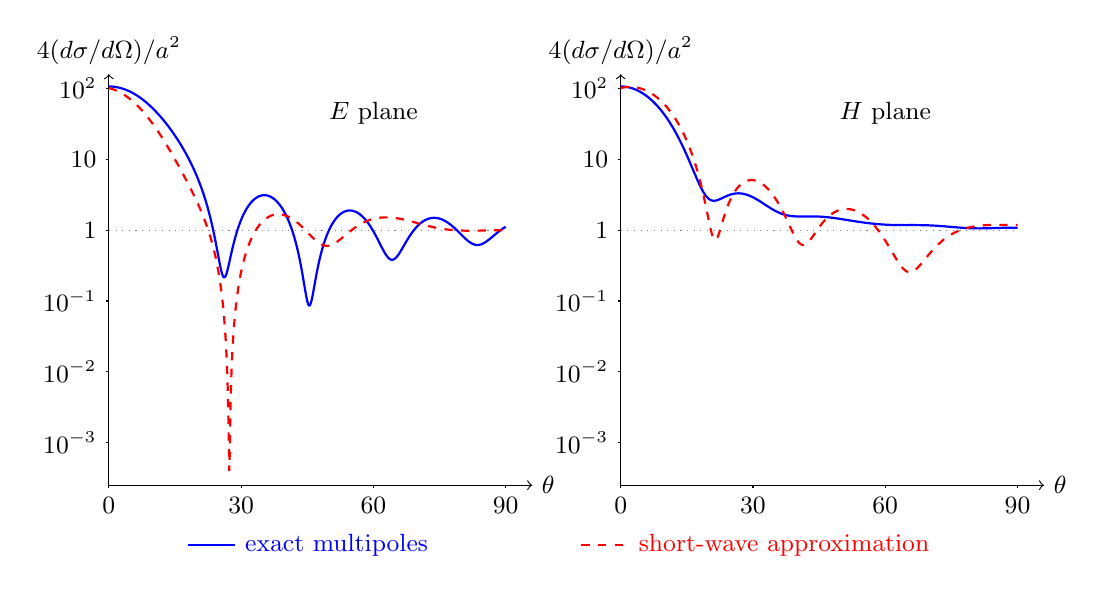
\begin{tikzpicture}[font=\small]
\begin{scope}[shift={(0.0cm,0)},x=.056cm,y=.9cm]
\draw[->] (0,-3.6) -- (96,-3.6) node[right] {$\theta$};
\draw[->] (0,-3.6) -- (0,2.2) node[above] {$4(d\sigma/d\Omega)/a^2$};
\draw (0,-3.6) -- ++(0,-0.035cm) node[below] {$0$};
\draw (30,-3.6) -- ++(0,-0.035cm) node[below] {$30$};
\draw (60,-3.6) -- ++(0,-0.035cm) node[below] {$60$};
\draw (90,-3.6) -- ++(0,-0.035cm) node[below] {$90$};
\draw (0,-3) -- ++(-0.035cm,0) node[left] {$10^{-3}$};
\draw (0,-2) -- ++(-0.035cm,0) node[left] {$10^{-2}$};
\draw (0,-1) -- ++(-0.035cm,0) node[left] {$10^{-1}$};
\draw (0,0) -- ++(-0.035cm,0) node[left] {$1$};
\draw (0,1) -- ++(-0.035cm,0) node[left] {$10$};
\draw (0,2) -- ++(-0.035cm,0) node[left] {$10^2$};
\draw[gray,dotted] (0,0)--(90,0);
\draw[blue,thick] plot coordinates {(0.00000,2.026771) (0.10000,2.026739) (0.20000,2.026644) (0.30000,2.026486) (0.40000,2.026265) (0.50000,2.025980) (0.60000,2.025632) (0.70000,2.025220) (0.80000,2.024746) (0.90000,2.024208) (1.00000,2.023607) (1.10000,2.022942) (1.20000,2.022215) (1.30000,2.021424) (1.40000,2.020570) (1.50000,2.019653) (1.60000,2.018672) (1.70000,2.017628) (1.80000,2.016522) (1.90000,2.015352) (2.00000,2.014119) (2.10000,2.012822) (2.20000,2.011463) (2.30000,2.010041) (2.40000,2.008555) (2.50000,2.007007) (2.60000,2.005395) (2.70000,2.003721) (2.80000,2.001983) (2.90000,2.000183) (3.00000,1.998320) (3.10000,1.996394) (3.20000,1.994405) (3.30000,1.992353) (3.40000,1.990238) (3.50000,1.988061) (3.60000,1.985821) (3.70000,1.983518) (3.80000,1.981153) (3.90000,1.978725) (4.00000,1.976234) (4.10000,1.973681) (4.20000,1.971065) (4.30000,1.968387) (4.40000,1.965647) (4.50000,1.962844) (4.60000,1.959978) (4.70000,1.957051) (4.80000,1.954061) (4.90000,1.951009) (5.00000,1.947895) (5.10000,1.944719) (5.20000,1.941481) (5.30000,1.938181) (5.40000,1.934819) (5.50000,1.931395) (5.60000,1.927909) (5.70000,1.924362) (5.80000,1.920752) (5.90000,1.917082) (6.00000,1.913349) (6.10000,1.909555) (6.20000,1.905700) (6.30000,1.901783) (6.40000,1.897805) (6.50000,1.893766) (6.60000,1.889666) (6.70000,1.885504) (6.80000,1.881282) (6.90000,1.876998) (7.00000,1.872654) (7.10000,1.868249) (7.20000,1.863783) (7.30000,1.859256) (7.40000,1.854669) (7.50000,1.850021) (7.60000,1.845313) (7.70000,1.840545) (7.80000,1.835716) (7.90000,1.830827) (8.00000,1.825878) (8.10000,1.820869) (8.20000,1.815800) (8.30000,1.810671) (8.40000,1.805483) (8.50000,1.800234) (8.60000,1.794926) (8.70000,1.789559) (8.80000,1.784132) (8.90000,1.778645) (9.00000,1.773099) (9.10000,1.767494) (9.20000,1.761830) (9.30000,1.756107) (9.40000,1.750324) (9.50000,1.744483) (9.60000,1.738583) (9.70000,1.732624) (9.80000,1.726606) (9.90000,1.720529) (10.00000,1.714394) (10.10000,1.708201) (10.20000,1.701948) (10.30000,1.695637) (10.40000,1.689268) (10.50000,1.682841) (10.60000,1.676355) (10.70000,1.669810) (10.80000,1.663208) (10.90000,1.656547) (11.00000,1.649827) (11.10000,1.643050) (11.20000,1.636214) (11.30000,1.629320) (11.40000,1.622367) (11.50000,1.615357) (11.60000,1.608287) (11.70000,1.601160) (11.80000,1.593974) (11.90000,1.586730) (12.00000,1.579427) (12.10000,1.572065) (12.20000,1.564644) (12.30000,1.557165) (12.40000,1.549627) (12.50000,1.542030) (12.60000,1.534373) (12.70000,1.526657) (12.80000,1.518881) (12.90000,1.511046) (13.00000,1.503151) (13.10000,1.495195) (13.20000,1.487179) (13.30000,1.479103) (13.40000,1.470965) (13.50000,1.462766) (13.60000,1.454505) (13.70000,1.446183) (13.80000,1.437798) (13.90000,1.429350) (14.00000,1.420839) (14.10000,1.412265) (14.20000,1.403626) (14.30000,1.394923) (14.40000,1.386155) (14.50000,1.377321) (14.60000,1.368421) (14.70000,1.359454) (14.80000,1.350419) (14.90000,1.341316) (15.00000,1.332144) (15.10000,1.322902) (15.20000,1.313590) (15.30000,1.304206) (15.40000,1.294750) (15.50000,1.285221) (15.60000,1.275618) (15.70000,1.265939) (15.80000,1.256184) (15.90000,1.246351) (16.00000,1.236440) (16.10000,1.226449) (16.20000,1.216377) (16.30000,1.206223) (16.40000,1.195984) (16.50000,1.185660) (16.60000,1.175250) (16.70000,1.164751) (16.80000,1.154162) (16.90000,1.143481) (17.00000,1.132707) (17.10000,1.121837) (17.20000,1.110870) (17.30000,1.099804) (17.40000,1.088636) (17.50000,1.077365) (17.60000,1.065988) (17.70000,1.054502) (17.80000,1.042906) (17.90000,1.031197) (18.00000,1.019372) (18.10000,1.007428) (18.20000,0.995363) (18.30000,0.983174) (18.40000,0.970857) (18.50000,0.958410) (18.60000,0.945829) (18.70000,0.933111) (18.80000,0.920252) (18.90000,0.907248) (19.00000,0.894096) (19.10000,0.880791) (19.20000,0.867330) (19.30000,0.853709) (19.40000,0.839922) (19.50000,0.825965) (19.60000,0.811834) (19.70000,0.797523) (19.80000,0.783027) (19.90000,0.768341) (20.00000,0.753459) (20.10000,0.738376) (20.20000,0.723085) (20.30000,0.707580) (20.40000,0.691855) (20.50000,0.675902) (20.60000,0.659716) (20.70000,0.643287) (20.80000,0.626610) (20.90000,0.609676) (21.00000,0.592476) (21.10000,0.575003) (21.20000,0.557246) (21.30000,0.539198) (21.40000,0.520849) (21.50000,0.502188) (21.60000,0.483205) (21.70000,0.463890) (21.80000,0.444231) (21.90000,0.424217) (22.00000,0.403837) (22.10000,0.383076) (22.20000,0.361924) (22.30000,0.340366) (22.40000,0.318390) (22.50000,0.295981) (22.60000,0.273126) (22.70000,0.249810) (22.80000,0.226018) (22.90000,0.201736) (23.00000,0.176950) (23.10000,0.151645) (23.20000,0.125808) (23.30000,0.099424) (23.40000,0.072483) (23.50000,0.044973) (23.60000,0.016886) (23.70000,-0.011784) (23.80000,-0.041041) (23.90000,-0.070882) (24.00000,-0.101299) (24.10000,-0.132279) (24.20000,-0.163797) (24.30000,-0.195819) (24.40000,-0.228297) (24.50000,-0.261164) (24.60000,-0.294335) (24.70000,-0.327699) (24.80000,-0.361115) (24.90000,-0.394409) (25.00000,-0.427366) (25.10000,-0.459729) (25.20000,-0.491194) (25.30000,-0.521406) (25.40000,-0.549967) (25.50000,-0.576438) (25.60000,-0.600358) (25.70000,-0.621255) (25.80000,-0.638681) (25.90000,-0.652238) (26.00000,-0.661609) (26.10000,-0.666591) (26.20000,-0.667109) (26.30000,-0.663229) (26.40000,-0.655148) (26.50000,-0.643174) (26.60000,-0.627703) (26.70000,-0.609183) (26.80000,-0.588084) (26.90000,-0.564872) (27.00000,-0.539988) (27.10000,-0.513837) (27.20000,-0.486776) (27.30000,-0.459115) (27.40000,-0.431116) (27.50000,-0.402998) (27.60000,-0.374941) (27.70000,-0.347087) (27.80000,-0.319551) (27.90000,-0.292423) (28.00000,-0.265770) (28.10000,-0.239645) (28.20000,-0.214083) (28.30000,-0.189110) (28.40000,-0.164743) (28.50000,-0.140992) (28.60000,-0.117859) (28.70000,-0.095344) (28.80000,-0.073443) (28.90000,-0.052147) (29.00000,-0.031448) (29.10000,-0.011335) (29.20000,0.008203) (29.30000,0.027179) (29.40000,0.045607) (29.50000,0.063498) (29.60000,0.080867) (29.70000,0.097726) (29.80000,0.114088) (29.90000,0.129967) (30.00000,0.145375) (30.10000,0.160324) (30.20000,0.174826) (30.30000,0.188892) (30.40000,0.202533) (30.50000,0.215760) (30.60000,0.228583) (30.70000,0.241012) (30.80000,0.253057) (30.90000,0.264725) (31.00000,0.276028) (31.10000,0.286971) (31.20000,0.297564) (31.30000,0.307814) (31.40000,0.317728) (31.50000,0.327313) (31.60000,0.336576) (31.70000,0.345524) (31.80000,0.354161) (31.90000,0.362495) (32.00000,0.370530) (32.10000,0.378271) (32.20000,0.385725) (32.30000,0.392895) (32.40000,0.399786) (32.50000,0.406403) (32.60000,0.412749) (32.70000,0.418829) (32.80000,0.424645) (32.90000,0.430203) (33.00000,0.435504) (33.10000,0.440553) (33.20000,0.445352) (33.30000,0.449905) (33.40000,0.454213) (33.50000,0.458280) (33.60000,0.462107) (33.70000,0.465697) (33.80000,0.469053) (33.90000,0.472176) (34.00000,0.475068) (34.10000,0.477731) (34.20000,0.480166) (34.30000,0.482376) (34.40000,0.484360) (34.50000,0.486122) (34.60000,0.487660) (34.70000,0.488978) (34.80000,0.490076) (34.90000,0.490954) (35.00000,0.491613) (35.10000,0.492055) (35.20000,0.492279) (35.30000,0.492286) (35.40000,0.492076) (35.50000,0.491649) (35.60000,0.491006) (35.70000,0.490147) (35.80000,0.489071) (35.90000,0.487779) (36.00000,0.486270) (36.10000,0.484543) (36.20000,0.482599) (36.30000,0.480436) (36.40000,0.478054) (36.50000,0.475453) (36.60000,0.472631) (36.70000,0.469588) (36.80000,0.466322) (36.90000,0.462832) (37.00000,0.459116) (37.10000,0.455175) (37.20000,0.451005) (37.30000,0.446605) (37.40000,0.441974) (37.50000,0.437109) (37.60000,0.432009) (37.70000,0.426672) (37.80000,0.421094) (37.90000,0.415274) (38.00000,0.409209) (38.10000,0.402897) (38.20000,0.396334) (38.30000,0.389518) (38.40000,0.382445) (38.50000,0.375112) (38.60000,0.367515) (38.70000,0.359651) (38.80000,0.351515) (38.90000,0.343104) (39.00000,0.334414) (39.10000,0.325439) (39.20000,0.316175) (39.30000,0.306616) (39.40000,0.296759) (39.50000,0.286596) (39.60000,0.276123) (39.70000,0.265332) (39.80000,0.254218) (39.90000,0.242774) (40.00000,0.230993) (40.10000,0.218867) (40.20000,0.206389) (40.30000,0.193550) (40.40000,0.180342) (40.50000,0.166756) (40.60000,0.152782) (40.70000,0.138410) (40.80000,0.123629) (40.90000,0.108430) (41.00000,0.092799) (41.10000,0.076726) (41.20000,0.060197) (41.30000,0.043199) (41.40000,0.025717) (41.50000,0.007737) (41.60000,-0.010756) (41.70000,-0.029779) (41.80000,-0.049348) (41.90000,-0.069482) (42.00000,-0.090199) (42.10000,-0.111519) (42.20000,-0.133461) (42.30000,-0.156046) (42.40000,-0.179296) (42.50000,-0.203233) (42.60000,-0.227879) (42.70000,-0.253258) (42.80000,-0.279392) (42.90000,-0.306303) (43.00000,-0.334014) (43.10000,-0.362545) (43.20000,-0.391913) (43.30000,-0.422135) (43.40000,-0.453221) (43.50000,-0.485175) (43.60000,-0.517992) (43.70000,-0.551659) (43.80000,-0.586144) (43.90000,-0.621398) (44.00000,-0.657346) (44.10000,-0.693881) (44.20000,-0.730857) (44.30000,-0.768076) (44.40000,-0.805280) (44.50000,-0.842139) (44.60000,-0.878238) (44.70000,-0.913073) (44.80000,-0.946043) (44.90000,-0.976463) (45.00000,-1.003582) (45.10000,-1.026621) (45.20000,-1.044833) (45.30000,-1.057569) (45.40000,-1.064353) (45.50000,-1.064942) (45.60000,-1.059360) (45.70000,-1.047892) (45.80000,-1.031049) (45.90000,-1.009501) (46.00000,-0.984005) (46.10000,-0.955339) (46.20000,-0.924245) (46.30000,-0.891396) (46.40000,-0.857375) (46.50000,-0.822671) (46.60000,-0.787684) (46.70000,-0.752731) (46.80000,-0.718059) (46.90000,-0.683856) (47.00000,-0.650261) (47.10000,-0.617375) (47.20000,-0.585268) (47.30000,-0.553985) (47.40000,-0.523555) (47.50000,-0.493991) (47.60000,-0.465294) (47.70000,-0.437460) (47.80000,-0.410477) (47.90000,-0.384329) (48.00000,-0.358998) (48.10000,-0.334463) (48.20000,-0.310701) (48.30000,-0.287691) (48.40000,-0.265409) (48.50000,-0.243833) (48.60000,-0.222940) (48.70000,-0.202708) (48.80000,-0.183116) (48.90000,-0.164142) (49.00000,-0.145768) (49.10000,-0.127974) (49.20000,-0.110741) (49.30000,-0.094052) (49.40000,-0.077890) (49.50000,-0.062238) (49.60000,-0.047082) (49.70000,-0.032407) (49.80000,-0.018199) (49.90000,-0.004444) (50.00000,0.008870) (50.10000,0.021756) (50.20000,0.034224) (50.30000,0.046286) (50.40000,0.057952) (50.50000,0.069232) (50.60000,0.080136) (50.70000,0.090672) (50.80000,0.100849) (50.90000,0.110675) (51.00000,0.120159) (51.10000,0.129307) (51.20000,0.138126) (51.30000,0.146624) (51.40000,0.154806) (51.50000,0.162679) (51.60000,0.170249) (51.70000,0.177521) (51.80000,0.184500) (51.90000,0.191192) (52.00000,0.197601) (52.10000,0.203732) (52.20000,0.209590) (52.30000,0.215178) (52.40000,0.220501) (52.50000,0.225562) (52.60000,0.230365) (52.70000,0.234914) (52.80000,0.239211) (52.90000,0.243260) (53.00000,0.247064) (53.10000,0.250625) (53.20000,0.253947) (53.30000,0.257032) (53.40000,0.259882) (53.50000,0.262500) (53.60000,0.264887) (53.70000,0.267047) (53.80000,0.268980) (53.90000,0.270689) (54.00000,0.272176) (54.10000,0.273442) (54.20000,0.274488) (54.30000,0.275317) (54.40000,0.275929) (54.50000,0.276326) (54.60000,0.276510) (54.70000,0.276480) (54.80000,0.276239) (54.90000,0.275786) (55.00000,0.275124) (55.10000,0.274253) (55.20000,0.273174) (55.30000,0.271886) (55.40000,0.270392) (55.50000,0.268692) (55.60000,0.266785) (55.70000,0.264673) (55.80000,0.262356) (55.90000,0.259834) (56.00000,0.257107) (56.10000,0.254177) (56.20000,0.251042) (56.30000,0.247703) (56.40000,0.244160) (56.50000,0.240414) (56.60000,0.236464) (56.70000,0.232310) (56.80000,0.227952) (56.90000,0.223391) (57.00000,0.218625) (57.10000,0.213656) (57.20000,0.208482) (57.30000,0.203104) (57.40000,0.197522) (57.50000,0.191736) (57.60000,0.185744) (57.70000,0.179548) (57.80000,0.173147) (57.90000,0.166541) (58.00000,0.159731) (58.10000,0.152715) (58.20000,0.145495) (58.30000,0.138070) (58.40000,0.130440) (58.50000,0.122607) (58.60000,0.114569) (58.70000,0.106329) (58.80000,0.097886) (58.90000,0.089242) (59.00000,0.080397) (59.10000,0.071352) (59.20000,0.062109) (59.30000,0.052671) (59.40000,0.043037) (59.50000,0.033212) (59.60000,0.023197) (59.70000,0.012996) (59.80000,0.002611) (59.90000,-0.007953) (60.00000,-0.018692) (60.10000,-0.029600) (60.20000,-0.040674) (60.30000,-0.051906) (60.40000,-0.063289) (60.50000,-0.074815) (60.60000,-0.086477) (60.70000,-0.098265) (60.80000,-0.110168) (60.90000,-0.122174) (61.00000,-0.134271) (61.10000,-0.146445) (61.20000,-0.158681) (61.30000,-0.170961) (61.40000,-0.183268) (61.50000,-0.195581) (61.60000,-0.207880) (61.70000,-0.220141) (61.80000,-0.232339) (61.90000,-0.244448) (62.00000,-0.256438) (62.10000,-0.268281) (62.20000,-0.279943) (62.30000,-0.291390) (62.40000,-0.302589) (62.50000,-0.313501) (62.60000,-0.324088) (62.70000,-0.334312) (62.80000,-0.344132) (62.90000,-0.353508) (63.00000,-0.362400) (63.10000,-0.370768) (63.20000,-0.378573) (63.30000,-0.385776) (63.40000,-0.392342) (63.50000,-0.398238) (63.60000,-0.403432) (63.70000,-0.407898) (63.80000,-0.411614) (63.90000,-0.414559) (64.00000,-0.416720) (64.10000,-0.418088) (64.20000,-0.418659) (64.30000,-0.418434) (64.40000,-0.417421) (64.50000,-0.415630) (64.60000,-0.413078) (64.70000,-0.409786) (64.80000,-0.405780) (64.90000,-0.401087) (65.00000,-0.395741) (65.10000,-0.389776) (65.20000,-0.383228) (65.30000,-0.376136) (65.40000,-0.368539) (65.50000,-0.360477) (65.60000,-0.351991) (65.70000,-0.343121) (65.80000,-0.333905) (65.90000,-0.324382) (66.00000,-0.314589) (66.10000,-0.304562) (66.20000,-0.294335) (66.30000,-0.283940) (66.40000,-0.273409) (66.50000,-0.262771) (66.60000,-0.252052) (66.70000,-0.241278) (66.80000,-0.230472) (66.90000,-0.219657) (67.00000,-0.208853) (67.10000,-0.198077) (67.20000,-0.187349) (67.30000,-0.176682) (67.40000,-0.166091) (67.50000,-0.155590) (67.60000,-0.145189) (67.70000,-0.134900) (67.80000,-0.124732) (67.90000,-0.114694) (68.00000,-0.104793) (68.10000,-0.095036) (68.20000,-0.085430) (68.30000,-0.075979) (68.40000,-0.066689) (68.50000,-0.057564) (68.60000,-0.048608) (68.70000,-0.039822) (68.80000,-0.031212) (68.90000,-0.022778) (69.00000,-0.014522) (69.10000,-0.006447) (69.20000,0.001447) (69.30000,0.009158) (69.40000,0.016686) (69.50000,0.024029) (69.60000,0.031189) (69.70000,0.038163) (69.80000,0.044953) (69.90000,0.051559) (70.00000,0.057980) (70.10000,0.064217) (70.20000,0.070270) (70.30000,0.076140) (70.40000,0.081828) (70.50000,0.087333) (70.60000,0.092658) (70.70000,0.097802) (70.80000,0.102766) (70.90000,0.107552) (71.00000,0.112160) (71.10000,0.116591) (71.20000,0.120846) (71.30000,0.124925) (71.40000,0.128831) (71.50000,0.132563) (71.60000,0.136124) (71.70000,0.139512) (71.80000,0.142731) (71.90000,0.145781) (72.00000,0.148662) (72.10000,0.151376) (72.20000,0.153924) (72.30000,0.156306) (72.40000,0.158524) (72.50000,0.160578) (72.60000,0.162471) (72.70000,0.164201) (72.80000,0.165771) (72.90000,0.167182) (73.00000,0.168434) (73.10000,0.169528) (73.20000,0.170465) (73.30000,0.171246) (73.40000,0.171872) (73.50000,0.172344) (73.60000,0.172662) (73.70000,0.172829) (73.80000,0.172843) (73.90000,0.172707) (74.00000,0.172422) (74.10000,0.171987) (74.20000,0.171404) (74.30000,0.170674) (74.40000,0.169798) (74.50000,0.168776) (74.60000,0.167610) (74.70000,0.166300) (74.80000,0.164847) (74.90000,0.163253) (75.00000,0.161518) (75.10000,0.159643) (75.20000,0.157628) (75.30000,0.155476) (75.40000,0.153187) (75.50000,0.150762) (75.60000,0.148202) (75.70000,0.145508) (75.80000,0.142682) (75.90000,0.139724) (76.00000,0.136636) (76.10000,0.133419) (76.20000,0.130074) (76.30000,0.126602) (76.40000,0.123006) (76.50000,0.119286) (76.60000,0.115445) (76.70000,0.111483) (76.80000,0.107402) (76.90000,0.103205) (77.00000,0.098892) (77.10000,0.094466) (77.20000,0.089929) (77.30000,0.085284) (77.40000,0.080531) (77.50000,0.075675) (77.60000,0.070716) (77.70000,0.065658) (77.80000,0.060504) (77.90000,0.055256) (78.00000,0.049918) (78.10000,0.044492) (78.20000,0.038982) (78.30000,0.033392) (78.40000,0.027725) (78.50000,0.021985) (78.60000,0.016177) (78.70000,0.010304) (78.80000,0.004372) (78.90000,-0.001616) (79.00000,-0.007654) (79.10000,-0.013737) (79.20000,-0.019860) (79.30000,-0.026016) (79.40000,-0.032200) (79.50000,-0.038406) (79.60000,-0.044628) (79.70000,-0.050857) (79.80000,-0.057089) (79.90000,-0.063315) (80.00000,-0.069527) (80.10000,-0.075719) (80.20000,-0.081882) (80.30000,-0.088007) (80.40000,-0.094087) (80.50000,-0.100113) (80.60000,-0.106075) (80.70000,-0.111965) (80.80000,-0.117773) (80.90000,-0.123490) (81.00000,-0.129106) (81.10000,-0.134612) (81.20000,-0.139997) (81.30000,-0.145251) (81.40000,-0.150366) (81.50000,-0.155331) (81.60000,-0.160136) (81.70000,-0.164771) (81.80000,-0.169228) (81.90000,-0.173497) (82.00000,-0.177568) (82.10000,-0.181433) (82.20000,-0.185085) (82.30000,-0.188513) (82.40000,-0.191712) (82.50000,-0.194674) (82.60000,-0.197392) (82.70000,-0.199861) (82.80000,-0.202075) (82.90000,-0.204030) (83.00000,-0.205721) (83.10000,-0.207146) (83.20000,-0.208302) (83.30000,-0.209187) (83.40000,-0.209800) (83.50000,-0.210142) (83.60000,-0.210212) (83.70000,-0.210012) (83.80000,-0.209545) (83.90000,-0.208812) (84.00000,-0.207819) (84.10000,-0.206569) (84.20000,-0.205066) (84.30000,-0.203318) (84.40000,-0.201329) (84.50000,-0.199107) (84.60000,-0.196659) (84.70000,-0.193992) (84.80000,-0.191115) (84.90000,-0.188035) (85.00000,-0.184763) (85.10000,-0.181306) (85.20000,-0.177675) (85.30000,-0.173877) (85.40000,-0.169923) (85.50000,-0.165822) (85.60000,-0.161584) (85.70000,-0.157218) (85.80000,-0.152734) (85.90000,-0.148141) (86.00000,-0.143448) (86.10000,-0.138665) (86.20000,-0.133801) (86.30000,-0.128863) (86.40000,-0.123862) (86.50000,-0.118804) (86.60000,-0.113700) (86.70000,-0.108555) (86.80000,-0.103379) (86.90000,-0.098177) (87.00000,-0.092959) (87.10000,-0.087729) (87.20000,-0.082496) (87.30000,-0.077265) (87.40000,-0.072042) (87.50000,-0.066833) (87.60000,-0.061644) (87.70000,-0.056480) (87.80000,-0.051346) (87.90000,-0.046247) (88.00000,-0.041187) (88.10000,-0.036170) (88.20000,-0.031201) (88.30000,-0.026284) (88.40000,-0.021422) (88.50000,-0.016618) (88.60000,-0.011877) (88.70000,-0.007200) (88.80000,-0.002591) (88.90000,0.001948) (89.00000,0.006413) (89.10000,0.010803) (89.20000,0.015116) (89.30000,0.019348) (89.40000,0.023499) (89.50000,0.027567) (89.60000,0.031550) (89.70000,0.035446) (89.80000,0.039254) (89.90000,0.042972) (90.00000,0.046600)};
\draw[red,dashed,thick] plot coordinates {(0.00000,2.004321) (0.10000,2.002784) (0.20000,2.001173) (0.30000,1.999489) (0.40000,1.997732) (0.50000,1.995902) (0.60000,1.993999) (0.70000,1.992023) (0.80000,1.989974) (0.90000,1.987852) (1.00000,1.985658) (1.10000,1.983391) (1.20000,1.981051) (1.30000,1.978639) (1.40000,1.976154) (1.50000,1.973596) (1.60000,1.970967) (1.70000,1.968264) (1.80000,1.965489) (1.90000,1.962642) (2.00000,1.959723) (2.10000,1.956731) (2.20000,1.953667) (2.30000,1.950531) (2.40000,1.947323) (2.50000,1.944042) (2.60000,1.940689) (2.70000,1.937264) (2.80000,1.933767) (2.90000,1.930198) (3.00000,1.926557) (3.10000,1.922844) (3.20000,1.919059) (3.30000,1.915201) (3.40000,1.911272) (3.50000,1.907271) (3.60000,1.903198) (3.70000,1.899053) (3.80000,1.894836) (3.90000,1.890548) (4.00000,1.886187) (4.10000,1.881755) (4.20000,1.877250) (4.30000,1.872674) (4.40000,1.868027) (4.50000,1.863307) (4.60000,1.858516) (4.70000,1.853653) (4.80000,1.848719) (4.90000,1.843713) (5.00000,1.838635) (5.10000,1.833486) (5.20000,1.828265) (5.30000,1.822973) (5.40000,1.817609) (5.50000,1.812174) (5.60000,1.806668) (5.70000,1.801090) (5.80000,1.795441) (5.90000,1.789720) (6.00000,1.783929) (6.10000,1.778066) (6.20000,1.772133) (6.30000,1.766128) (6.40000,1.760052) (6.50000,1.753906) (6.60000,1.747689) (6.70000,1.741401) (6.80000,1.735042) (6.90000,1.728613) (7.00000,1.722114) (7.10000,1.715544) (7.20000,1.708904) (7.30000,1.702194) (7.40000,1.695413) (7.50000,1.688563) (7.60000,1.681643) (7.70000,1.674654) (7.80000,1.667595) (7.90000,1.660467) (8.00000,1.653269) (8.10000,1.646002) (8.20000,1.638667) (8.30000,1.631263) (8.40000,1.623790) (8.50000,1.616249) (8.60000,1.608640) (8.70000,1.600963) (8.80000,1.593218) (8.90000,1.585405) (9.00000,1.577526) (9.10000,1.569579) (9.20000,1.561566) (9.30000,1.553486) (9.40000,1.545340) (9.50000,1.537128) (9.60000,1.528851) (9.70000,1.520508) (9.80000,1.512100) (9.90000,1.503628) (10.00000,1.495091) (10.10000,1.486490) (10.20000,1.477825) (10.30000,1.469098) (10.40000,1.460307) (10.50000,1.451454) (10.60000,1.442539) (10.70000,1.433562) (10.80000,1.424524) (10.90000,1.415426) (11.00000,1.406267) (11.10000,1.397048) (11.20000,1.387770) (11.30000,1.378434) (11.40000,1.369039) (11.50000,1.359586) (11.60000,1.350076) (11.70000,1.340510) (11.80000,1.330887) (11.90000,1.321209) (12.00000,1.311476) (12.10000,1.301689) (12.20000,1.291848) (12.30000,1.281954) (12.40000,1.272008) (12.50000,1.262010) (12.60000,1.251961) (12.70000,1.241861) (12.80000,1.231712) (12.90000,1.221514) (13.00000,1.211267) (13.10000,1.200972) (13.20000,1.190631) (13.30000,1.180243) (13.40000,1.169810) (13.50000,1.159332) (13.60000,1.148810) (13.70000,1.138245) (13.80000,1.127637) (13.90000,1.116987) (14.00000,1.106296) (14.10000,1.095564) (14.20000,1.084792) (14.30000,1.073982) (14.40000,1.063132) (14.50000,1.052246) (14.60000,1.041321) (14.70000,1.030361) (14.80000,1.019365) (14.90000,1.008333) (15.00000,0.997267) (15.10000,0.986167) (15.20000,0.975033) (15.30000,0.963866) (15.40000,0.952666) (15.50000,0.941434) (15.60000,0.930170) (15.70000,0.918875) (15.80000,0.907549) (15.90000,0.896192) (16.00000,0.884804) (16.10000,0.873385) (16.20000,0.861936) (16.30000,0.850457) (16.40000,0.838947) (16.50000,0.827407) (16.60000,0.815836) (16.70000,0.804234) (16.80000,0.792600) (16.90000,0.780935) (17.00000,0.769238) (17.10000,0.757508) (17.20000,0.745745) (17.30000,0.733947) (17.40000,0.722115) (17.50000,0.710246) (17.60000,0.698341) (17.70000,0.686397) (17.80000,0.674413) (17.90000,0.662389) (18.00000,0.650322) (18.10000,0.638212) (18.20000,0.626055) (18.30000,0.613850) (18.40000,0.601595) (18.50000,0.589289) (18.60000,0.576928) (18.70000,0.564509) (18.80000,0.552032) (18.90000,0.539491) (19.00000,0.526886) (19.10000,0.514212) (19.20000,0.501466) (19.30000,0.488644) (19.40000,0.475744) (19.50000,0.462761) (19.60000,0.449691) (19.70000,0.436530) (19.80000,0.423273) (19.90000,0.409915) (20.00000,0.396453) (20.10000,0.382880) (20.20000,0.369192) (20.30000,0.355383) (20.40000,0.341446) (20.50000,0.327376) (20.60000,0.313167) (20.70000,0.298811) (20.80000,0.284303) (20.90000,0.269634) (21.00000,0.254796) (21.10000,0.239783) (21.20000,0.224586) (21.30000,0.209196) (21.40000,0.193603) (21.50000,0.177800) (21.60000,0.161774) (21.70000,0.145517) (21.80000,0.129017) (21.90000,0.112263) (22.00000,0.095242) (22.10000,0.077942) (22.20000,0.060350) (22.30000,0.042452) (22.40000,0.024232) (22.50000,0.005676) (22.60000,-0.013234) (22.70000,-0.032515) (22.80000,-0.052185) (22.90000,-0.072265) (23.00000,-0.092774) (23.10000,-0.113736) (23.20000,-0.135174) (23.30000,-0.157114) (23.40000,-0.179582) (23.50000,-0.202609) (23.60000,-0.226225) (23.70000,-0.250464) (23.80000,-0.275363) (23.90000,-0.300962) (24.00000,-0.327303) (24.10000,-0.354433) (24.20000,-0.382402) (24.30000,-0.411268) (24.40000,-0.441091) (24.50000,-0.471938) (24.60000,-0.503884) (24.70000,-0.537012) (24.80000,-0.571415) (24.90000,-0.607195) (25.00000,-0.644468) (25.10000,-0.683366) (25.20000,-0.724038) (25.30000,-0.766653) (25.40000,-0.811408) (25.50000,-0.858529) (25.60000,-0.908281) (25.70000,-0.960975) (25.80000,-1.016981) (25.90000,-1.076743) (26.00000,-1.140802) (26.10000,-1.209821) (26.20000,-1.284633) (26.30000,-1.366295) (26.40000,-1.456181) (26.50000,-1.556124) (26.60000,-1.668631) (26.70000,-1.797261) (26.80000,-1.947282) (26.90000,-2.126895) (27.00000,-2.349614) (27.10000,-2.638568) (27.20000,-3.025441) (27.30000,-3.399693) (27.40000,-3.182097) (27.50000,-2.766161) (27.60000,-2.448758) (27.70000,-2.208693) (27.80000,-2.018465) (27.90000,-1.861785) (28.00000,-1.728951) (28.10000,-1.613853) (28.20000,-1.512430) (28.30000,-1.421862) (28.40000,-1.340114) (28.50000,-1.265671) (28.60000,-1.197378) (28.70000,-1.134335) (28.80000,-1.075825) (28.90000,-1.021271) (29.00000,-0.970198) (29.10000,-0.922216) (29.20000,-0.876995) (29.30000,-0.834256) (29.40000,-0.793763) (29.50000,-0.755311) (29.60000,-0.718722) (29.70000,-0.683844) (29.80000,-0.650540) (29.90000,-0.618690) (30.00000,-0.588190) (30.10000,-0.558945) (30.20000,-0.530870) (30.30000,-0.503890) (30.40000,-0.477937) (30.50000,-0.452949) (30.60000,-0.428870) (30.70000,-0.405650) (30.80000,-0.383241) (30.90000,-0.361602) (31.00000,-0.340694) (31.10000,-0.320480) (31.20000,-0.300928) (31.30000,-0.282008) (31.40000,-0.263690) (31.50000,-0.245950) (31.60000,-0.228762) (31.70000,-0.212105) (31.80000,-0.195956) (31.90000,-0.180298) (32.00000,-0.165110) (32.10000,-0.150377) (32.20000,-0.136081) (32.30000,-0.122209) (32.40000,-0.108745) (32.50000,-0.095677) (32.60000,-0.082991) (32.70000,-0.070676) (32.80000,-0.058721) (32.90000,-0.047115) (33.00000,-0.035849) (33.10000,-0.024912) (33.20000,-0.014296) (33.30000,-0.003992) (33.40000,0.006008) (33.50000,0.015711) (33.60000,0.025125) (33.70000,0.034256) (33.80000,0.043112) (33.90000,0.051699) (34.00000,0.060022) (34.10000,0.068087) (34.20000,0.075900) (34.30000,0.083467) (34.40000,0.090791) (34.50000,0.097878) (34.60000,0.104732) (34.70000,0.111358) (34.80000,0.117759) (34.90000,0.123941) (35.00000,0.129906) (35.10000,0.135659) (35.20000,0.141202) (35.30000,0.146540) (35.40000,0.151676) (35.50000,0.156612) (35.60000,0.161352) (35.70000,0.165899) (35.80000,0.170255) (35.90000,0.174423) (36.00000,0.178406) (36.10000,0.182206) (36.20000,0.185826) (36.30000,0.189267) (36.40000,0.192533) (36.50000,0.195625) (36.60000,0.198546) (36.70000,0.201297) (36.80000,0.203880) (36.90000,0.206297) (37.00000,0.208551) (37.10000,0.210642) (37.20000,0.212573) (37.30000,0.214345) (37.40000,0.215959) (37.50000,0.217418) (37.60000,0.218722) (37.70000,0.219874) (37.80000,0.220874) (37.90000,0.221724) (38.00000,0.222426) (38.10000,0.222980) (38.20000,0.223388) (38.30000,0.223651) (38.40000,0.223770) (38.50000,0.223747) (38.60000,0.223582) (38.70000,0.223277) (38.80000,0.222833) (38.90000,0.222250) (39.00000,0.221531) (39.10000,0.220675) (39.20000,0.219685) (39.30000,0.218560) (39.40000,0.217302) (39.50000,0.215912) (39.60000,0.214391) (39.70000,0.212740) (39.80000,0.210959) (39.90000,0.209050) (40.00000,0.207014) (40.10000,0.204852) (40.20000,0.202564) (40.30000,0.200151) (40.40000,0.197615) (40.50000,0.194957) (40.60000,0.192177) (40.70000,0.189276) (40.80000,0.186256) (40.90000,0.183117) (41.00000,0.179861) (41.10000,0.176488) (41.20000,0.173000) (41.30000,0.169398) (41.40000,0.165682) (41.50000,0.161855) (41.60000,0.157917) (41.70000,0.153870) (41.80000,0.149714) (41.90000,0.145452) (42.00000,0.141084) (42.10000,0.136613) (42.20000,0.132039) (42.30000,0.127364) (42.40000,0.122590) (42.50000,0.117718) (42.60000,0.112751) (42.70000,0.107690) (42.80000,0.102538) (42.90000,0.097295) (43.00000,0.091965) (43.10000,0.086550) (43.20000,0.081051) (43.30000,0.075472) (43.40000,0.069815) (43.50000,0.064082) (43.60000,0.058277) (43.70000,0.052402) (43.80000,0.046461) (43.90000,0.040457) (44.00000,0.034393) (44.10000,0.028273) (44.20000,0.022100) (44.30000,0.015878) (44.40000,0.009612) (44.50000,0.003306) (44.60000,-0.003036) (44.70000,-0.009410) (44.80000,-0.015810) (44.90000,-0.022232) (45.00000,-0.028670) (45.10000,-0.035118) (45.20000,-0.041572) (45.30000,-0.048025) (45.40000,-0.054472) (45.50000,-0.060905) (45.60000,-0.067320) (45.70000,-0.073707) (45.80000,-0.080062) (45.90000,-0.086377) (46.00000,-0.092644) (46.10000,-0.098857) (46.20000,-0.105007) (46.30000,-0.111086) (46.40000,-0.117088) (46.50000,-0.123003) (46.60000,-0.128823) (46.70000,-0.134541) (46.80000,-0.140147) (46.90000,-0.145634) (47.00000,-0.150992) (47.10000,-0.156214) (47.20000,-0.161291) (47.30000,-0.166215) (47.40000,-0.170977) (47.50000,-0.175570) (47.60000,-0.179984) (47.70000,-0.184214) (47.80000,-0.188251) (47.90000,-0.192087) (48.00000,-0.195717) (48.10000,-0.199132) (48.20000,-0.202329) (48.30000,-0.205299) (48.40000,-0.208039) (48.50000,-0.210544) (48.60000,-0.212808) (48.70000,-0.214829) (48.80000,-0.216604) (48.90000,-0.218129) (49.00000,-0.219403) (49.10000,-0.220424) (49.20000,-0.221192) (49.30000,-0.221707) (49.40000,-0.221969) (49.50000,-0.221979) (49.60000,-0.221739) (49.70000,-0.221252) (49.80000,-0.220520) (49.90000,-0.219547) (50.00000,-0.218337) (50.10000,-0.216894) (50.20000,-0.215224) (50.30000,-0.213332) (50.40000,-0.211223) (50.50000,-0.208905) (50.60000,-0.206384) (50.70000,-0.203666) (50.80000,-0.200758) (50.90000,-0.197669) (51.00000,-0.194405) (51.10000,-0.190975) (51.20000,-0.187385) (51.30000,-0.183645) (51.40000,-0.179762) (51.50000,-0.175744) (51.60000,-0.171598) (51.70000,-0.167334) (51.80000,-0.162958) (51.90000,-0.158479) (52.00000,-0.153903) (52.10000,-0.149240) (52.20000,-0.144495) (52.30000,-0.139677) (52.40000,-0.134792) (52.50000,-0.129847) (52.60000,-0.124849) (52.70000,-0.119805) (52.80000,-0.114720) (52.90000,-0.109600) (53.00000,-0.104453) (53.10000,-0.099282) (53.20000,-0.094094) (53.30000,-0.088894) (53.40000,-0.083687) (53.50000,-0.078477) (53.60000,-0.073270) (53.70000,-0.068069) (53.80000,-0.062879) (53.90000,-0.057703) (54.00000,-0.052546) (54.10000,-0.047411) (54.20000,-0.042301) (54.30000,-0.037220) (54.40000,-0.032171) (54.50000,-0.027155) (54.60000,-0.022178) (54.70000,-0.017239) (54.80000,-0.012343) (54.90000,-0.007492) (55.00000,-0.002687) (55.10000,0.002070) (55.20000,0.006776) (55.30000,0.011430) (55.40000,0.016031) (55.50000,0.020576) (55.60000,0.025065) (55.70000,0.029495) (55.80000,0.033867) (55.90000,0.038179) (56.00000,0.042429) (56.10000,0.046617) (56.20000,0.050743) (56.30000,0.054805) (56.40000,0.058802) (56.50000,0.062734) (56.60000,0.066601) (56.70000,0.070401) (56.80000,0.074135) (56.90000,0.077802) (57.00000,0.081402) (57.10000,0.084934) (57.20000,0.088399) (57.30000,0.091796) (57.40000,0.095124) (57.50000,0.098384) (57.60000,0.101576) (57.70000,0.104700) (57.80000,0.107755) (57.90000,0.110742) (58.00000,0.113661) (58.10000,0.116512) (58.20000,0.119294) (58.30000,0.122009) (58.40000,0.124656) (58.50000,0.127236) (58.60000,0.129748) (58.70000,0.132194) (58.80000,0.134572) (58.90000,0.136884) (59.00000,0.139130) (59.10000,0.141310) (59.20000,0.143425) (59.30000,0.145474) (59.40000,0.147458) (59.50000,0.149378) (59.60000,0.151234) (59.70000,0.153026) (59.80000,0.154754) (59.90000,0.156420) (60.00000,0.158023) (60.10000,0.159564) (60.20000,0.161043) (60.30000,0.162462) (60.40000,0.163819) (60.50000,0.165117) (60.60000,0.166354) (60.70000,0.167532) (60.80000,0.168652) (60.90000,0.169713) (61.00000,0.170716) (61.10000,0.171662) (61.20000,0.172551) (61.30000,0.173384) (61.40000,0.174161) (61.50000,0.174883) (61.60000,0.175550) (61.70000,0.176163) (61.80000,0.176723) (61.90000,0.177229) (62.00000,0.177683) (62.10000,0.178084) (62.20000,0.178435) (62.30000,0.178734) (62.40000,0.178983) (62.50000,0.179183) (62.60000,0.179333) (62.70000,0.179435) (62.80000,0.179488) (62.90000,0.179495) (63.00000,0.179454) (63.10000,0.179367) (63.20000,0.179235) (63.30000,0.179057) (63.40000,0.178835) (63.50000,0.178569) (63.60000,0.178260) (63.70000,0.177908) (63.80000,0.177514) (63.90000,0.177079) (64.00000,0.176603) (64.10000,0.176086) (64.20000,0.175531) (64.30000,0.174936) (64.40000,0.174303) (64.50000,0.173632) (64.60000,0.172924) (64.70000,0.172179) (64.80000,0.171399) (64.90000,0.170584) (65.00000,0.169734) (65.10000,0.168851) (65.20000,0.167934) (65.30000,0.166984) (65.40000,0.166003) (65.50000,0.164991) (65.60000,0.163948) (65.70000,0.162875) (65.80000,0.161772) (65.90000,0.160642) (66.00000,0.159483) (66.10000,0.158297) (66.20000,0.157084) (66.30000,0.155846) (66.40000,0.154582) (66.50000,0.153294) (66.60000,0.151982) (66.70000,0.150647) (66.80000,0.149289) (66.90000,0.147909) (67.00000,0.146509) (67.10000,0.145088) (67.20000,0.143647) (67.30000,0.142187) (67.40000,0.140709) (67.50000,0.139213) (67.60000,0.137700) (67.70000,0.136171) (67.80000,0.134626) (67.90000,0.133067) (68.00000,0.131493) (68.10000,0.129906) (68.20000,0.128306) (68.30000,0.126693) (68.40000,0.125070) (68.50000,0.123435) (68.60000,0.121791) (68.70000,0.120137) (68.80000,0.118475) (68.90000,0.116805) (69.00000,0.115127) (69.10000,0.113443) (69.20000,0.111752) (69.30000,0.110057) (69.40000,0.108357) (69.50000,0.106653) (69.60000,0.104945) (69.70000,0.103236) (69.80000,0.101524) (69.90000,0.099811) (70.00000,0.098097) (70.10000,0.096383) (70.20000,0.094670) (70.30000,0.092958) (70.40000,0.091249) (70.50000,0.089541) (70.60000,0.087837) (70.70000,0.086137) (70.80000,0.084441) (70.90000,0.082749) (71.00000,0.081064) (71.10000,0.079384) (71.20000,0.077712) (71.30000,0.076046) (71.40000,0.074388) (71.50000,0.072739) (71.60000,0.071098) (71.70000,0.069467) (71.80000,0.067846) (71.90000,0.066235) (72.00000,0.064636) (72.10000,0.063047) (72.20000,0.061471) (72.30000,0.059907) (72.40000,0.058355) (72.50000,0.056817) (72.60000,0.055293) (72.70000,0.053782) (72.80000,0.052286) (72.90000,0.050805) (73.00000,0.049340) (73.10000,0.047890) (73.20000,0.046455) (73.30000,0.045038) (73.40000,0.043637) (73.50000,0.042252) (73.60000,0.040886) (73.70000,0.039536) (73.80000,0.038205) (73.90000,0.036891) (74.00000,0.035596) (74.10000,0.034320) (74.20000,0.033062) (74.30000,0.031824) (74.40000,0.030604) (74.50000,0.029404) (74.60000,0.028224) (74.70000,0.027063) (74.80000,0.025922) (74.90000,0.024801) (75.00000,0.023700) (75.10000,0.022619) (75.20000,0.021558) (75.30000,0.020518) (75.40000,0.019498) (75.50000,0.018498) (75.60000,0.017519) (75.70000,0.016561) (75.80000,0.015622) (75.90000,0.014705) (76.00000,0.013807) (76.10000,0.012930) (76.20000,0.012074) (76.30000,0.011238) (76.40000,0.010422) (76.50000,0.009626) (76.60000,0.008850) (76.70000,0.008094) (76.80000,0.007358) (76.90000,0.006642) (77.00000,0.005945) (77.10000,0.005268) (77.20000,0.004610) (77.30000,0.003972) (77.40000,0.003352) (77.50000,0.002751) (77.60000,0.002169) (77.70000,0.001606) (77.80000,0.001060) (77.90000,0.000533) (78.00000,0.000023) (78.10000,-0.000469) (78.20000,-0.000943) (78.30000,-0.001400) (78.40000,-0.001841) (78.50000,-0.002264) (78.60000,-0.002672) (78.70000,-0.003063) (78.80000,-0.003438) (78.90000,-0.003797) (79.00000,-0.004141) (79.10000,-0.004470) (79.20000,-0.004783) (79.30000,-0.005083) (79.40000,-0.005367) (79.50000,-0.005638) (79.60000,-0.005895) (79.70000,-0.006138) (79.80000,-0.006368) (79.90000,-0.006586) (80.00000,-0.006790) (80.10000,-0.006982) (80.20000,-0.007162) (80.30000,-0.007330) (80.40000,-0.007486) (80.50000,-0.007631) (80.60000,-0.007765) (80.70000,-0.007888) (80.80000,-0.008001) (80.90000,-0.008104) (81.00000,-0.008196) (81.10000,-0.008279) (81.20000,-0.008353) (81.30000,-0.008418) (81.40000,-0.008473) (81.50000,-0.008520) (81.60000,-0.008559) (81.70000,-0.008590) (81.80000,-0.008613) (81.90000,-0.008628) (82.00000,-0.008636) (82.10000,-0.008637) (82.20000,-0.008631) (82.30000,-0.008618) (82.40000,-0.008599) (82.50000,-0.008574) (82.60000,-0.008543) (82.70000,-0.008507) (82.80000,-0.008465) (82.90000,-0.008417) (83.00000,-0.008365) (83.10000,-0.008308) (83.20000,-0.008246) (83.30000,-0.008179) (83.40000,-0.008109) (83.50000,-0.008034) (83.60000,-0.007955) (83.70000,-0.007873) (83.80000,-0.007787) (83.90000,-0.007698) (84.00000,-0.007606) (84.10000,-0.007511) (84.20000,-0.007412) (84.30000,-0.007311) (84.40000,-0.007208) (84.50000,-0.007102) (84.60000,-0.006994) (84.70000,-0.006883) (84.80000,-0.006771) (84.90000,-0.006656) (85.00000,-0.006540) (85.10000,-0.006422) (85.20000,-0.006303) (85.30000,-0.006182) (85.40000,-0.006060) (85.50000,-0.005936) (85.60000,-0.005812) (85.70000,-0.005686) (85.80000,-0.005559) (85.90000,-0.005432) (86.00000,-0.005303) (86.10000,-0.005174) (86.20000,-0.005044) (86.30000,-0.004914) (86.40000,-0.004783) (86.50000,-0.004651) (86.60000,-0.004519) (86.70000,-0.004387) (86.80000,-0.004255) (86.90000,-0.004122) (87.00000,-0.003989) (87.10000,-0.003855) (87.20000,-0.003722) (87.30000,-0.003588) (87.40000,-0.003455) (87.50000,-0.003321) (87.60000,-0.003187) (87.70000,-0.003054) (87.80000,-0.002920) (87.90000,-0.002786) (88.00000,-0.002653) (88.10000,-0.002519) (88.20000,-0.002386) (88.30000,-0.002252) (88.40000,-0.002119) (88.50000,-0.001986) (88.60000,-0.001853) (88.70000,-0.001720) (88.80000,-0.001587) (88.90000,-0.001454) (89.00000,-0.001321) (89.10000,-0.001189) (89.20000,-0.001056) (89.30000,-0.000924) (89.40000,-0.000792) (89.50000,-0.000660) (89.60000,-0.000528) (89.70000,-0.000396) (89.80000,-0.000264) (89.90000,-0.000132) (90.00000,0.000000)};
\node at (60,1.65) {$E$ plane};
\end{scope}
\begin{scope}[shift={(6.5cm,0)},x=.056cm,y=.9cm]
\draw[->] (0,-3.6) -- (96,-3.6) node[right] {$\theta$};
\draw[->] (0,-3.6) -- (0,2.2) node[above] {$4(d\sigma/d\Omega)/a^2$};
\draw (0,-3.6) -- ++(0,-0.035cm) node[below] {$0$};
\draw (30,-3.6) -- ++(0,-0.035cm) node[below] {$30$};
\draw (60,-3.6) -- ++(0,-0.035cm) node[below] {$60$};
\draw (90,-3.6) -- ++(0,-0.035cm) node[below] {$90$};
\draw (0,-3) -- ++(-0.035cm,0) node[left] {$10^{-3}$};
\draw (0,-2) -- ++(-0.035cm,0) node[left] {$10^{-2}$};
\draw (0,-1) -- ++(-0.035cm,0) node[left] {$10^{-1}$};
\draw (0,0) -- ++(-0.035cm,0) node[left] {$1$};
\draw (0,1) -- ++(-0.035cm,0) node[left] {$10$};
\draw (0,2) -- ++(-0.035cm,0) node[left] {$10^2$};
\draw[gray,dotted] (0,0)--(90,0);
\draw[blue,thick] plot coordinates {(0.00000,2.026771) (0.10000,2.026733) (0.20000,2.026618) (0.30000,2.026426) (0.40000,2.026157) (0.50000,2.025812) (0.60000,2.025390) (0.70000,2.024892) (0.80000,2.024316) (0.90000,2.023664) (1.00000,2.022935) (1.10000,2.022129) (1.20000,2.021246) (1.30000,2.020286) (1.40000,2.019248) (1.50000,2.018134) (1.60000,2.016943) (1.70000,2.015674) (1.80000,2.014327) (1.90000,2.012904) (2.00000,2.011402) (2.10000,2.009823) (2.20000,2.008167) (2.30000,2.006432) (2.40000,2.004620) (2.50000,2.002729) (2.60000,2.000760) (2.70000,1.998713) (2.80000,1.996587) (2.90000,1.994383) (3.00000,1.992100) (3.10000,1.989738) (3.20000,1.987297) (3.30000,1.984777) (3.40000,1.982178) (3.50000,1.979499) (3.60000,1.976740) (3.70000,1.973901) (3.80000,1.970982) (3.90000,1.967983) (4.00000,1.964904) (4.10000,1.961744) (4.20000,1.958503) (4.30000,1.955181) (4.40000,1.951777) (4.50000,1.948292) (4.60000,1.944726) (4.70000,1.941077) (4.80000,1.937346) (4.90000,1.933533) (5.00000,1.929636) (5.10000,1.925657) (5.20000,1.921595) (5.30000,1.917449) (5.40000,1.913219) (5.50000,1.908905) (5.60000,1.904506) (5.70000,1.900023) (5.80000,1.895455) (5.90000,1.890802) (6.00000,1.886063) (6.10000,1.881238) (6.20000,1.876326) (6.30000,1.871328) (6.40000,1.866243) (6.50000,1.861071) (6.60000,1.855811) (6.70000,1.850463) (6.80000,1.845026) (6.90000,1.839501) (7.00000,1.833887) (7.10000,1.828183) (7.20000,1.822389) (7.30000,1.816504) (7.40000,1.810529) (7.50000,1.804462) (7.60000,1.798304) (7.70000,1.792054) (7.80000,1.785712) (7.90000,1.779276) (8.00000,1.772747) (8.10000,1.766124) (8.20000,1.759406) (8.30000,1.752594) (8.40000,1.745687) (8.50000,1.738684) (8.60000,1.731584) (8.70000,1.724388) (8.80000,1.717094) (8.90000,1.709703) (9.00000,1.702213) (9.10000,1.694625) (9.20000,1.686937) (9.30000,1.679149) (9.40000,1.671261) (9.50000,1.663272) (9.60000,1.655181) (9.70000,1.646988) (9.80000,1.638693) (9.90000,1.630294) (10.00000,1.621792) (10.10000,1.613185) (10.20000,1.604473) (10.30000,1.595657) (10.40000,1.586734) (10.50000,1.577704) (10.60000,1.568567) (10.70000,1.559323) (10.80000,1.549971) (10.90000,1.540509) (11.00000,1.530938) (11.10000,1.521258) (11.20000,1.511467) (11.30000,1.501565) (11.40000,1.491552) (11.50000,1.481426) (11.60000,1.471189) (11.70000,1.460838) (11.80000,1.450374) (11.90000,1.439796) (12.00000,1.429104) (12.10000,1.418298) (12.20000,1.407377) (12.30000,1.396340) (12.40000,1.385188) (12.50000,1.373920) (12.60000,1.362536) (12.70000,1.351036) (12.80000,1.339419) (12.90000,1.327687) (13.00000,1.315838) (13.10000,1.303872) (13.20000,1.291791) (13.30000,1.279594) (13.40000,1.267281) (13.50000,1.254854) (13.60000,1.242311) (13.70000,1.229655) (13.80000,1.216885) (13.90000,1.204003) (14.00000,1.191009) (14.10000,1.177905) (14.20000,1.164693) (14.30000,1.151372) (14.40000,1.137946) (14.50000,1.124416) (14.60000,1.110784) (14.70000,1.097052) (14.80000,1.083223) (14.90000,1.069300) (15.00000,1.055286) (15.10000,1.041184) (15.20000,1.026998) (15.30000,1.012733) (15.40000,0.998391) (15.50000,0.983979) (15.60000,0.969502) (15.70000,0.954965) (15.80000,0.940374) (15.90000,0.925736) (16.00000,0.911058) (16.10000,0.896348) (16.20000,0.881613) (16.30000,0.866863) (16.40000,0.852108) (16.50000,0.837356) (16.60000,0.822619) (16.70000,0.807908) (16.80000,0.793234) (16.90000,0.778612) (17.00000,0.764053) (17.10000,0.749572) (17.20000,0.735184) (17.30000,0.720904) (17.40000,0.706748) (17.50000,0.692732) (17.60000,0.678874) (17.70000,0.665192) (17.80000,0.651704) (17.90000,0.638429) (18.00000,0.625384) (18.10000,0.612591) (18.20000,0.600067) (18.30000,0.587833) (18.40000,0.575907) (18.50000,0.564309) (18.60000,0.553057) (18.70000,0.542169) (18.80000,0.531663) (18.90000,0.521554) (19.00000,0.511859) (19.10000,0.502591) (19.20000,0.493764) (19.30000,0.485389) (19.40000,0.477475) (19.50000,0.470032) (19.60000,0.463065) (19.70000,0.456579) (19.80000,0.450576) (19.90000,0.445057) (20.00000,0.440021) (20.10000,0.435463) (20.20000,0.431379) (20.30000,0.427762) (20.40000,0.424602) (20.50000,0.421889) (20.60000,0.419610) (20.70000,0.417753) (20.80000,0.416302) (20.90000,0.415241) (21.00000,0.414554) (21.10000,0.414223) (21.20000,0.414228) (21.30000,0.414553) (21.40000,0.415176) (21.50000,0.416080) (21.60000,0.417244) (21.70000,0.418649) (21.80000,0.420276) (21.90000,0.422107) (22.00000,0.424122) (22.10000,0.426303) (22.20000,0.428634) (22.30000,0.431096) (22.40000,0.433674) (22.50000,0.436352) (22.60000,0.439114) (22.70000,0.441947) (22.80000,0.444835) (22.90000,0.447767) (23.00000,0.450730) (23.10000,0.453712) (23.20000,0.456703) (23.30000,0.459691) (23.40000,0.462667) (23.50000,0.465622) (23.60000,0.468548) (23.70000,0.471436) (23.80000,0.474280) (23.90000,0.477072) (24.00000,0.479805) (24.10000,0.482475) (24.20000,0.485076) (24.30000,0.487602) (24.40000,0.490049) (24.50000,0.492414) (24.60000,0.494691) (24.70000,0.496878) (24.80000,0.498972) (24.90000,0.500969) (25.00000,0.502868) (25.10000,0.504665) (25.20000,0.506359) (25.30000,0.507948) (25.40000,0.509430) (25.50000,0.510805) (25.60000,0.512070) (25.70000,0.513225) (25.80000,0.514269) (25.90000,0.515201) (26.00000,0.516022) (26.10000,0.516729) (26.20000,0.517324) (26.30000,0.517805) (26.40000,0.518174) (26.50000,0.518430) (26.60000,0.518573) (26.70000,0.518603) (26.80000,0.518522) (26.90000,0.518329) (27.00000,0.518025) (27.10000,0.517610) (27.20000,0.517086) (27.30000,0.516453) (27.40000,0.515711) (27.50000,0.514863) (27.60000,0.513908) (27.70000,0.512847) (27.80000,0.511683) (27.90000,0.510415) (28.00000,0.509046) (28.10000,0.507575) (28.20000,0.506005) (28.30000,0.504337) (28.40000,0.502572) (28.50000,0.500711) (28.60000,0.498757) (28.70000,0.496709) (28.80000,0.494571) (28.90000,0.492344) (29.00000,0.490028) (29.10000,0.487626) (29.20000,0.485140) (29.30000,0.482571) (29.40000,0.479921) (29.50000,0.477191) (29.60000,0.474384) (29.70000,0.471502) (29.80000,0.468546) (29.90000,0.465519) (30.00000,0.462421) (30.10000,0.459257) (30.20000,0.456026) (30.30000,0.452733) (30.40000,0.449378) (30.50000,0.445964) (30.60000,0.442494) (30.70000,0.438969) (30.80000,0.435392) (30.90000,0.431765) (31.00000,0.428091) (31.10000,0.424372) (31.20000,0.420610) (31.30000,0.416808) (31.40000,0.412969) (31.50000,0.409095) (31.60000,0.405189) (31.70000,0.401254) (31.80000,0.397291) (31.90000,0.393304) (32.00000,0.389296) (32.10000,0.385268) (32.20000,0.381225) (32.30000,0.377169) (32.40000,0.373102) (32.50000,0.369028) (32.60000,0.364949) (32.70000,0.360869) (32.80000,0.356789) (32.90000,0.352714) (33.00000,0.348645) (33.10000,0.344586) (33.20000,0.340539) (33.30000,0.336508) (33.40000,0.332495) (33.50000,0.328503) (33.60000,0.324535) (33.70000,0.320594) (33.80000,0.316682) (33.90000,0.312802) (34.00000,0.308957) (34.10000,0.305149) (34.20000,0.301382) (34.30000,0.297656) (34.40000,0.293976) (34.50000,0.290344) (34.60000,0.286761) (34.70000,0.283230) (34.80000,0.279753) (34.90000,0.276333) (35.00000,0.272971) (35.10000,0.269669) (35.20000,0.266430) (35.30000,0.263254) (35.40000,0.260144) (35.50000,0.257100) (35.60000,0.254125) (35.70000,0.251220) (35.80000,0.248386) (35.90000,0.245624) (36.00000,0.242935) (36.10000,0.240319) (36.20000,0.237779) (36.30000,0.235313) (36.40000,0.232923) (36.50000,0.230609) (36.60000,0.228371) (36.70000,0.226210) (36.80000,0.224125) (36.90000,0.222116) (37.00000,0.220183) (37.10000,0.218326) (37.20000,0.216544) (37.30000,0.214837) (37.40000,0.213204) (37.50000,0.211643) (37.60000,0.210155) (37.70000,0.208739) (37.80000,0.207392) (37.90000,0.206115) (38.00000,0.204905) (38.10000,0.203762) (38.20000,0.202684) (38.30000,0.201670) (38.40000,0.200717) (38.50000,0.199825) (38.60000,0.198992) (38.70000,0.198217) (38.80000,0.197496) (38.90000,0.196829) (39.00000,0.196214) (39.10000,0.195649) (39.20000,0.195132) (39.30000,0.194662) (39.40000,0.194235) (39.50000,0.193851) (39.60000,0.193507) (39.70000,0.193202) (39.80000,0.192934) (39.90000,0.192700) (40.00000,0.192498) (40.10000,0.192328) (40.20000,0.192186) (40.30000,0.192072) (40.40000,0.191983) (40.50000,0.191917) (40.60000,0.191872) (40.70000,0.191847) (40.80000,0.191841) (40.90000,0.191850) (41.00000,0.191874) (41.10000,0.191911) (41.20000,0.191960) (41.30000,0.192018) (41.40000,0.192084) (41.50000,0.192157) (41.60000,0.192236) (41.70000,0.192318) (41.80000,0.192403) (41.90000,0.192489) (42.00000,0.192575) (42.10000,0.192660) (42.20000,0.192742) (42.30000,0.192821) (42.40000,0.192895) (42.50000,0.192963) (42.60000,0.193025) (42.70000,0.193079) (42.80000,0.193124) (42.90000,0.193160) (43.00000,0.193185) (43.10000,0.193199) (43.20000,0.193202) (43.30000,0.193192) (43.40000,0.193169) (43.50000,0.193132) (43.60000,0.193081) (43.70000,0.193015) (43.80000,0.192933) (43.90000,0.192836) (44.00000,0.192722) (44.10000,0.192592) (44.20000,0.192444) (44.30000,0.192279) (44.40000,0.192097) (44.50000,0.191897) (44.60000,0.191679) (44.70000,0.191442) (44.80000,0.191187) (44.90000,0.190914) (45.00000,0.190622) (45.10000,0.190311) (45.20000,0.189981) (45.30000,0.189633) (45.40000,0.189266) (45.50000,0.188880) (45.60000,0.188475) (45.70000,0.188052) (45.80000,0.187610) (45.90000,0.187150) (46.00000,0.186671) (46.10000,0.186174) (46.20000,0.185660) (46.30000,0.185127) (46.40000,0.184577) (46.50000,0.184010) (46.60000,0.183425) (46.70000,0.182824) (46.80000,0.182205) (46.90000,0.181571) (47.00000,0.180920) (47.10000,0.180254) (47.20000,0.179572) (47.30000,0.178875) (47.40000,0.178163) (47.50000,0.177437) (47.60000,0.176696) (47.70000,0.175942) (47.80000,0.175174) (47.90000,0.174393) (48.00000,0.173599) (48.10000,0.172793) (48.20000,0.171975) (48.30000,0.171146) (48.40000,0.170305) (48.50000,0.169453) (48.60000,0.168590) (48.70000,0.167718) (48.80000,0.166836) (48.90000,0.165944) (49.00000,0.165044) (49.10000,0.164135) (49.20000,0.163218) (49.30000,0.162293) (49.40000,0.161361) (49.50000,0.160421) (49.60000,0.159476) (49.70000,0.158523) (49.80000,0.157565) (49.90000,0.156602) (50.00000,0.155633) (50.10000,0.154660) (50.20000,0.153682) (50.30000,0.152700) (50.40000,0.151714) (50.50000,0.150725) (50.60000,0.149733) (50.70000,0.148739) (50.80000,0.147742) (50.90000,0.146743) (51.00000,0.145743) (51.10000,0.144741) (51.20000,0.143738) (51.30000,0.142734) (51.40000,0.141730) (51.50000,0.140726) (51.60000,0.139723) (51.70000,0.138719) (51.80000,0.137717) (51.90000,0.136715) (52.00000,0.135715) (52.10000,0.134717) (52.20000,0.133720) (52.30000,0.132726) (52.40000,0.131733) (52.50000,0.130744) (52.60000,0.129757) (52.70000,0.128774) (52.80000,0.127794) (52.90000,0.126817) (53.00000,0.125844) (53.10000,0.124876) (53.20000,0.123911) (53.30000,0.122951) (53.40000,0.121996) (53.50000,0.121045) (53.60000,0.120100) (53.70000,0.119160) (53.80000,0.118225) (53.90000,0.117295) (54.00000,0.116372) (54.10000,0.115455) (54.20000,0.114543) (54.30000,0.113638) (54.40000,0.112740) (54.50000,0.111848) (54.60000,0.110963) (54.70000,0.110085) (54.80000,0.109214) (54.90000,0.108350) (55.00000,0.107494) (55.10000,0.106645) (55.20000,0.105804) (55.30000,0.104971) (55.40000,0.104145) (55.50000,0.103328) (55.60000,0.102519) (55.70000,0.101719) (55.80000,0.100927) (55.90000,0.100143) (56.00000,0.099369) (56.10000,0.098603) (56.20000,0.097846) (56.30000,0.097098) (56.40000,0.096360) (56.50000,0.095631) (56.60000,0.094911) (56.70000,0.094201) (56.80000,0.093500) (56.90000,0.092809) (57.00000,0.092128) (57.10000,0.091457) (57.20000,0.090796) (57.30000,0.090146) (57.40000,0.089505) (57.50000,0.088875) (57.60000,0.088255) (57.70000,0.087645) (57.80000,0.087046) (57.90000,0.086458) (58.00000,0.085880) (58.10000,0.085313) (58.20000,0.084757) (58.30000,0.084212) (58.40000,0.083677) (58.50000,0.083154) (58.60000,0.082641) (58.70000,0.082140) (58.80000,0.081650) (58.90000,0.081170) (59.00000,0.080702) (59.10000,0.080245) (59.20000,0.079799) (59.30000,0.079365) (59.40000,0.078941) (59.50000,0.078529) (59.60000,0.078128) (59.70000,0.077738) (59.80000,0.077359) (59.90000,0.076992) (60.00000,0.076635) (60.10000,0.076289) (60.20000,0.075955) (60.30000,0.075631) (60.40000,0.075318) (60.50000,0.075017) (60.60000,0.074725) (60.70000,0.074445) (60.80000,0.074175) (60.90000,0.073916) (61.00000,0.073667) (61.10000,0.073428) (61.20000,0.073200) (61.30000,0.072981) (61.40000,0.072773) (61.50000,0.072574) (61.60000,0.072386) (61.70000,0.072206) (61.80000,0.072036) (61.90000,0.071875) (62.00000,0.071724) (62.10000,0.071581) (62.20000,0.071446) (62.30000,0.071321) (62.40000,0.071203) (62.50000,0.071094) (62.60000,0.070993) (62.70000,0.070899) (62.80000,0.070813) (62.90000,0.070733) (63.00000,0.070661) (63.10000,0.070596) (63.20000,0.070537) (63.30000,0.070485) (63.40000,0.070438) (63.50000,0.070397) (63.60000,0.070362) (63.70000,0.070332) (63.80000,0.070307) (63.90000,0.070286) (64.00000,0.070270) (64.10000,0.070258) (64.20000,0.070250) (64.30000,0.070245) (64.40000,0.070244) (64.50000,0.070245) (64.60000,0.070249) (64.70000,0.070256) (64.80000,0.070264) (64.90000,0.070274) (65.00000,0.070286) (65.10000,0.070299) (65.20000,0.070312) (65.30000,0.070326) (65.40000,0.070340) (65.50000,0.070355) (65.60000,0.070368) (65.70000,0.070381) (65.80000,0.070393) (65.90000,0.070404) (66.00000,0.070413) (66.10000,0.070420) (66.20000,0.070425) (66.30000,0.070427) (66.40000,0.070427) (66.50000,0.070424) (66.60000,0.070417) (66.70000,0.070406) (66.80000,0.070392) (66.90000,0.070373) (67.00000,0.070350) (67.10000,0.070322) (67.20000,0.070290) (67.30000,0.070252) (67.40000,0.070208) (67.50000,0.070159) (67.60000,0.070104) (67.70000,0.070043) (67.80000,0.069975) (67.90000,0.069901) (68.00000,0.069820) (68.10000,0.069732) (68.20000,0.069637) (68.30000,0.069534) (68.40000,0.069424) (68.50000,0.069306) (68.60000,0.069181) (68.70000,0.069047) (68.80000,0.068905) (68.90000,0.068755) (69.00000,0.068596) (69.10000,0.068429) (69.20000,0.068253) (69.30000,0.068068) (69.40000,0.067875) (69.50000,0.067673) (69.60000,0.067461) (69.70000,0.067241) (69.80000,0.067011) (69.90000,0.066773) (70.00000,0.066525) (70.10000,0.066268) (70.20000,0.066002) (70.30000,0.065727) (70.40000,0.065442) (70.50000,0.065148) (70.60000,0.064845) (70.70000,0.064533) (70.80000,0.064212) (70.90000,0.063882) (71.00000,0.063543) (71.10000,0.063195) (71.20000,0.062839) (71.30000,0.062474) (71.40000,0.062100) (71.50000,0.061717) (71.60000,0.061327) (71.70000,0.060928) (71.80000,0.060521) (71.90000,0.060107) (72.00000,0.059684) (72.10000,0.059255) (72.20000,0.058817) (72.30000,0.058373) (72.40000,0.057922) (72.50000,0.057463) (72.60000,0.056999) (72.70000,0.056528) (72.80000,0.056051) (72.90000,0.055568) (73.00000,0.055080) (73.10000,0.054586) (73.20000,0.054087) (73.30000,0.053584) (73.40000,0.053075) (73.50000,0.052563) (73.60000,0.052047) (73.70000,0.051527) (73.80000,0.051004) (73.90000,0.050477) (74.00000,0.049948) (74.10000,0.049417) (74.20000,0.048883) (74.30000,0.048348) (74.40000,0.047811) (74.50000,0.047273) (74.60000,0.046734) (74.70000,0.046195) (74.80000,0.045656) (74.90000,0.045116) (75.00000,0.044578) (75.10000,0.044040) (75.20000,0.043504) (75.30000,0.042969) (75.40000,0.042436) (75.50000,0.041906) (75.60000,0.041378) (75.70000,0.040853) (75.80000,0.040331) (75.90000,0.039813) (76.00000,0.039299) (76.10000,0.038789) (76.20000,0.038284) (76.30000,0.037784) (76.40000,0.037289) (76.50000,0.036799) (76.60000,0.036316) (76.70000,0.035839) (76.80000,0.035368) (76.90000,0.034905) (77.00000,0.034448) (77.10000,0.033999) (77.20000,0.033557) (77.30000,0.033123) (77.40000,0.032698) (77.50000,0.032281) (77.60000,0.031873) (77.70000,0.031474) (77.80000,0.031084) (77.90000,0.030703) (78.00000,0.030332) (78.10000,0.029971) (78.20000,0.029619) (78.30000,0.029278) (78.40000,0.028948) (78.50000,0.028628) (78.60000,0.028318) (78.70000,0.028020) (78.80000,0.027732) (78.90000,0.027455) (79.00000,0.027190) (79.10000,0.026935) (79.20000,0.026692) (79.30000,0.026461) (79.40000,0.026241) (79.50000,0.026032) (79.60000,0.025835) (79.70000,0.025649) (79.80000,0.025475) (79.90000,0.025313) (80.00000,0.025162) (80.10000,0.025023) (80.20000,0.024895) (80.30000,0.024778) (80.40000,0.024673) (80.50000,0.024579) (80.60000,0.024497) (80.70000,0.024425) (80.80000,0.024364) (80.90000,0.024314) (81.00000,0.024275) (81.10000,0.024247) (81.20000,0.024229) (81.30000,0.024221) (81.40000,0.024223) (81.50000,0.024236) (81.60000,0.024257) (81.70000,0.024289) (81.80000,0.024330) (81.90000,0.024379) (82.00000,0.024438) (82.10000,0.024505) (82.20000,0.024581) (82.30000,0.024664) (82.40000,0.024756) (82.50000,0.024855) (82.60000,0.024961) (82.70000,0.025075) (82.80000,0.025195) (82.90000,0.025322) (83.00000,0.025454) (83.10000,0.025593) (83.20000,0.025737) (83.30000,0.025887) (83.40000,0.026041) (83.50000,0.026200) (83.60000,0.026363) (83.70000,0.026530) (83.80000,0.026701) (83.90000,0.026875) (84.00000,0.027052) (84.10000,0.027232) (84.20000,0.027414) (84.30000,0.027598) (84.40000,0.027784) (84.50000,0.027971) (84.60000,0.028159) (84.70000,0.028348) (84.80000,0.028537) (84.90000,0.028726) (85.00000,0.028915) (85.10000,0.029103) (85.20000,0.029290) (85.30000,0.029477) (85.40000,0.029661) (85.50000,0.029844) (85.60000,0.030025) (85.70000,0.030203) (85.80000,0.030378) (85.90000,0.030551) (86.00000,0.030720) (86.10000,0.030885) (86.20000,0.031047) (86.30000,0.031204) (86.40000,0.031357) (86.50000,0.031506) (86.60000,0.031649) (86.70000,0.031787) (86.80000,0.031920) (86.90000,0.032048) (87.00000,0.032169) (87.10000,0.032285) (87.20000,0.032394) (87.30000,0.032497) (87.40000,0.032593) (87.50000,0.032682) (87.60000,0.032764) (87.70000,0.032839) (87.80000,0.032907) (87.90000,0.032967) (88.00000,0.033020) (88.10000,0.033065) (88.20000,0.033102) (88.30000,0.033130) (88.40000,0.033151) (88.50000,0.033164) (88.60000,0.033168) (88.70000,0.033164) (88.80000,0.033151) (88.90000,0.033130) (89.00000,0.033100) (89.10000,0.033061) (89.20000,0.033014) (89.30000,0.032958) (89.40000,0.032893) (89.50000,0.032820) (89.60000,0.032737) (89.70000,0.032646) (89.80000,0.032547) (89.90000,0.032438) (90.00000,0.032321)};
\draw[red,dashed,thick] plot coordinates {(0.00000,2.004321) (0.10000,2.005787) (0.20000,2.007182) (0.30000,2.008506) (0.40000,2.009759) (0.50000,2.010941) (0.60000,2.012052) (0.70000,2.013091) (0.80000,2.014060) (0.90000,2.014956) (1.00000,2.015782) (1.10000,2.016535) (1.20000,2.017217) (1.30000,2.017827) (1.40000,2.018364) (1.50000,2.018830) (1.60000,2.019223) (1.70000,2.019544) (1.80000,2.019792) (1.90000,2.019968) (2.00000,2.020071) (2.10000,2.020100) (2.20000,2.020057) (2.30000,2.019940) (2.40000,2.019750) (2.50000,2.019486) (2.60000,2.019148) (2.70000,2.018736) (2.80000,2.018250) (2.90000,2.017690) (3.00000,2.017055) (3.10000,2.016345) (3.20000,2.015561) (3.30000,2.014701) (3.40000,2.013766) (3.50000,2.012755) (3.60000,2.011669) (3.70000,2.010506) (3.80000,2.009267) (3.90000,2.007952) (4.00000,2.006560) (4.10000,2.005091) (4.20000,2.003545) (4.30000,2.001921) (4.40000,2.000220) (4.50000,1.998440) (4.60000,1.996582) (4.70000,1.994646) (4.80000,1.992631) (4.90000,1.990536) (5.00000,1.988362) (5.10000,1.986108) (5.20000,1.983774) (5.30000,1.981360) (5.40000,1.978864) (5.50000,1.976288) (5.60000,1.973630) (5.70000,1.970890) (5.80000,1.968068) (5.90000,1.965164) (6.00000,1.962176) (6.10000,1.959105) (6.20000,1.955950) (6.30000,1.952711) (6.40000,1.949387) (6.50000,1.945978) (6.60000,1.942484) (6.70000,1.938904) (6.80000,1.935237) (6.90000,1.931483) (7.00000,1.927642) (7.10000,1.923713) (7.20000,1.919695) (7.30000,1.915589) (7.40000,1.911393) (7.50000,1.907106) (7.60000,1.902730) (7.70000,1.898262) (7.80000,1.893702) (7.90000,1.889050) (8.00000,1.884305) (8.10000,1.879466) (8.20000,1.874533) (8.30000,1.869506) (8.40000,1.864382) (8.50000,1.859162) (8.60000,1.853845) (8.70000,1.848431) (8.80000,1.842917) (8.90000,1.837305) (9.00000,1.831592) (9.10000,1.825779) (9.20000,1.819864) (9.30000,1.813846) (9.40000,1.807725) (9.50000,1.801500) (9.60000,1.795169) (9.70000,1.788733) (9.80000,1.782189) (9.90000,1.775537) (10.00000,1.768776) (10.10000,1.761905) (10.20000,1.754922) (10.30000,1.747828) (10.40000,1.740620) (10.50000,1.733297) (10.60000,1.725859) (10.70000,1.718303) (10.80000,1.710630) (10.90000,1.702837) (11.00000,1.694924) (11.10000,1.686888) (11.20000,1.678729) (11.30000,1.670445) (11.40000,1.662034) (11.50000,1.653496) (11.60000,1.644829) (11.70000,1.636030) (11.80000,1.627099) (11.90000,1.618033) (12.00000,1.608832) (12.10000,1.599492) (12.20000,1.590013) (12.30000,1.580393) (12.40000,1.570629) (12.50000,1.560720) (12.60000,1.550663) (12.70000,1.540457) (12.80000,1.530099) (12.90000,1.519587) (13.00000,1.508919) (13.10000,1.498092) (13.20000,1.487103) (13.30000,1.475952) (13.40000,1.464633) (13.50000,1.453146) (13.60000,1.441487) (13.70000,1.429653) (13.80000,1.417642) (13.90000,1.405450) (14.00000,1.393074) (14.10000,1.380511) (14.20000,1.367758) (14.30000,1.354810) (14.40000,1.341665) (14.50000,1.328319) (14.60000,1.314767) (14.70000,1.301006) (14.80000,1.287032) (14.90000,1.272841) (15.00000,1.258427) (15.10000,1.243787) (15.20000,1.228916) (15.30000,1.213809) (15.40000,1.198461) (15.50000,1.182866) (15.60000,1.167020) (15.70000,1.150916) (15.80000,1.134550) (15.90000,1.117914) (16.00000,1.101003) (16.10000,1.083811) (16.20000,1.066331) (16.30000,1.048556) (16.40000,1.030479) (16.50000,1.012094) (16.60000,0.993392) (16.70000,0.974366) (16.80000,0.955008) (16.90000,0.935310) (17.00000,0.915265) (17.10000,0.894864) (17.20000,0.874097) (17.30000,0.852958) (17.40000,0.831436) (17.50000,0.809524) (17.60000,0.787213) (17.70000,0.764494) (17.80000,0.741359) (17.90000,0.717799) (18.00000,0.693808) (18.10000,0.669378) (18.20000,0.644502) (18.30000,0.619175) (18.40000,0.593394) (18.50000,0.567156) (18.60000,0.540460) (18.70000,0.513309) (18.80000,0.485707) (18.90000,0.457664) (19.00000,0.429193) (19.10000,0.400312) (19.20000,0.371048) (19.30000,0.341434) (19.40000,0.311513) (19.50000,0.281338) (19.60000,0.250976) (19.70000,0.220510) (19.80000,0.190036) (19.90000,0.159675) (20.00000,0.129566) (20.10000,0.099872) (20.20000,0.070781) (20.30000,0.042508) (20.40000,0.015290) (20.50000,-0.010612) (20.60000,-0.034920) (20.70000,-0.057343) (20.80000,-0.077593) (20.90000,-0.095388) (21.00000,-0.110476) (21.10000,-0.122640) (21.20000,-0.131716) (21.30000,-0.137607) (21.40000,-0.140283) (21.50000,-0.139791) (21.60000,-0.136244) (21.70000,-0.129819) (21.80000,-0.120742) (21.90000,-0.109276) (22.00000,-0.095702) (22.10000,-0.080314) (22.20000,-0.063398) (22.30000,-0.045229) (22.40000,-0.026065) (22.50000,-0.006139) (22.60000,0.014342) (22.70000,0.035195) (22.80000,0.056261) (22.90000,0.077406) (23.00000,0.098515) (23.10000,0.119493) (23.20000,0.140263) (23.30000,0.160759) (23.40000,0.180931) (23.50000,0.200737) (23.60000,0.220146) (23.70000,0.239134) (23.80000,0.257682) (23.90000,0.275779) (24.00000,0.293415) (24.10000,0.310585) (24.20000,0.327289) (24.30000,0.343527) (24.40000,0.359301) (24.50000,0.374615) (24.60000,0.389474) (24.70000,0.403884) (24.80000,0.417854) (24.90000,0.431388) (25.00000,0.444497) (25.10000,0.457187) (25.20000,0.469467) (25.30000,0.481344) (25.40000,0.492829) (25.50000,0.503928) (25.60000,0.514649) (25.70000,0.525002) (25.80000,0.534993) (25.90000,0.544631) (26.00000,0.553923) (26.10000,0.562875) (26.20000,0.571497) (26.30000,0.579794) (26.40000,0.587772) (26.50000,0.595440) (26.60000,0.602802) (26.70000,0.609865) (26.80000,0.616635) (26.90000,0.623117) (27.00000,0.629317) (27.10000,0.635240) (27.20000,0.640891) (27.30000,0.646275) (27.40000,0.651397) (27.50000,0.656261) (27.60000,0.660871) (27.70000,0.665232) (27.80000,0.669348) (27.90000,0.673222) (28.00000,0.676859) (28.10000,0.680261) (28.20000,0.683432) (28.30000,0.686376) (28.40000,0.689096) (28.50000,0.691593) (28.60000,0.693873) (28.70000,0.695937) (28.80000,0.697787) (28.90000,0.699427) (29.00000,0.700859) (29.10000,0.702085) (29.20000,0.703107) (29.30000,0.703928) (29.40000,0.704550) (29.50000,0.704973) (29.60000,0.705202) (29.70000,0.705236) (29.80000,0.705078) (29.90000,0.704730) (30.00000,0.704193) (30.10000,0.703468) (30.20000,0.702556) (30.30000,0.701460) (30.40000,0.700180) (30.50000,0.698717) (30.60000,0.697073) (30.70000,0.695249) (30.80000,0.693245) (30.90000,0.691062) (31.00000,0.688702) (31.10000,0.686165) (31.20000,0.683451) (31.30000,0.680562) (31.40000,0.677499) (31.50000,0.674261) (31.60000,0.670849) (31.70000,0.667264) (31.80000,0.663506) (31.90000,0.659575) (32.00000,0.655472) (32.10000,0.651198) (32.20000,0.646752) (32.30000,0.642135) (32.40000,0.637346) (32.50000,0.632387) (32.60000,0.627256) (32.70000,0.621955) (32.80000,0.616483) (32.90000,0.610840) (33.00000,0.605026) (33.10000,0.599042) (33.20000,0.592886) (33.30000,0.586560) (33.40000,0.580063) (33.50000,0.573394) (33.60000,0.566554) (33.70000,0.559543) (33.80000,0.552360) (33.90000,0.545005) (34.00000,0.537479) (34.10000,0.529780) (34.20000,0.521909) (34.30000,0.513866) (34.40000,0.505651) (34.50000,0.497263) (34.60000,0.488702) (34.70000,0.479969) (34.80000,0.471063) (34.90000,0.461985) (35.00000,0.452734) (35.10000,0.443312) (35.20000,0.433717) (35.30000,0.423952) (35.40000,0.414015) (35.50000,0.403908) (35.60000,0.393632) (35.70000,0.383187) (35.80000,0.372574) (35.90000,0.361795) (36.00000,0.350851) (36.10000,0.339744) (36.20000,0.328476) (36.30000,0.317048) (36.40000,0.305464) (36.50000,0.293727) (36.60000,0.281838) (36.70000,0.269803) (36.80000,0.257625) (36.90000,0.245308) (37.00000,0.232858) (37.10000,0.220280) (37.20000,0.207580) (37.30000,0.194766) (37.40000,0.181844) (37.50000,0.168823) (37.60000,0.155713) (37.70000,0.142523) (37.80000,0.129264) (37.90000,0.115948) (38.00000,0.102589) (38.10000,0.089200) (38.20000,0.075796) (38.30000,0.062396) (38.40000,0.049015) (38.50000,0.035675) (38.60000,0.022395) (38.70000,0.009197) (38.80000,-0.003895) (38.90000,-0.016855) (39.00000,-0.029659) (39.10000,-0.042277) (39.20000,-0.054680) (39.30000,-0.066840) (39.40000,-0.078723) (39.50000,-0.090297) (39.60000,-0.101530) (39.70000,-0.112387) (39.80000,-0.122835) (39.90000,-0.132839) (40.00000,-0.142365) (40.10000,-0.151381) (40.20000,-0.159855) (40.30000,-0.167755) (40.40000,-0.175054) (40.50000,-0.181724) (40.60000,-0.187742) (40.70000,-0.193087) (40.80000,-0.197741) (40.90000,-0.201690) (41.00000,-0.204925) (41.10000,-0.207440) (41.20000,-0.209232) (41.30000,-0.210304) (41.40000,-0.210663) (41.50000,-0.210319) (41.60000,-0.209286) (41.70000,-0.207583) (41.80000,-0.205230) (41.90000,-0.202251) (42.00000,-0.198674) (42.10000,-0.194527) (42.20000,-0.189840) (42.30000,-0.184647) (42.40000,-0.178979) (42.50000,-0.172870) (42.60000,-0.166355) (42.70000,-0.159466) (42.80000,-0.152237) (42.90000,-0.144701) (43.00000,-0.136891) (43.10000,-0.128836) (43.20000,-0.120567) (43.30000,-0.112111) (43.40000,-0.103498) (43.50000,-0.094752) (43.60000,-0.085897) (43.70000,-0.076957) (43.80000,-0.067953) (43.90000,-0.058905) (44.00000,-0.049832) (44.10000,-0.040752) (44.20000,-0.031679) (44.30000,-0.022630) (44.40000,-0.013618) (44.50000,-0.004654) (44.60000,0.004248) (44.70000,0.013079) (44.80000,0.021830) (44.90000,0.030491) (45.00000,0.039056) (45.10000,0.047516) (45.20000,0.055865) (45.30000,0.064099) (45.40000,0.072211) (45.50000,0.080197) (45.60000,0.088054) (45.70000,0.095777) (45.80000,0.103363) (45.90000,0.110810) (46.00000,0.118116) (46.10000,0.125278) (46.20000,0.132295) (46.30000,0.139165) (46.40000,0.145887) (46.50000,0.152460) (46.60000,0.158883) (46.70000,0.165156) (46.80000,0.171279) (46.90000,0.177250) (47.00000,0.183070) (47.10000,0.188740) (47.20000,0.194258) (47.30000,0.199626) (47.40000,0.204843) (47.50000,0.209911) (47.60000,0.214829) (47.70000,0.219598) (47.80000,0.224218) (47.90000,0.228691) (48.00000,0.233016) (48.10000,0.237195) (48.20000,0.241229) (48.30000,0.245117) (48.40000,0.248862) (48.50000,0.252463) (48.60000,0.255921) (48.70000,0.259238) (48.80000,0.262414) (48.90000,0.265449) (49.00000,0.268346) (49.10000,0.271104) (49.20000,0.273724) (49.30000,0.276208) (49.40000,0.278556) (49.50000,0.280769) (49.60000,0.282848) (49.70000,0.284793) (49.80000,0.286605) (49.90000,0.288285) (50.00000,0.289835) (50.10000,0.291254) (50.20000,0.292543) (50.30000,0.293703) (50.40000,0.294736) (50.50000,0.295640) (50.60000,0.296418) (50.70000,0.297070) (50.80000,0.297596) (50.90000,0.297998) (51.00000,0.298275) (51.10000,0.298428) (51.20000,0.298459) (51.30000,0.298367) (51.40000,0.298153) (51.50000,0.297818) (51.60000,0.297362) (51.70000,0.296785) (51.80000,0.296089) (51.90000,0.295273) (52.00000,0.294338) (52.10000,0.293285) (52.20000,0.292113) (52.30000,0.290824) (52.40000,0.289418) (52.50000,0.287894) (52.60000,0.286254) (52.70000,0.284498) (52.80000,0.282626) (52.90000,0.280638) (53.00000,0.278535) (53.10000,0.276316) (53.20000,0.273983) (53.30000,0.271535) (53.40000,0.268973) (53.50000,0.266297) (53.60000,0.263506) (53.70000,0.260602) (53.80000,0.257585) (53.90000,0.254453) (54.00000,0.251209) (54.10000,0.247851) (54.20000,0.244380) (54.30000,0.240797) (54.40000,0.237100) (54.50000,0.233291) (54.60000,0.229369) (54.70000,0.225334) (54.80000,0.221186) (54.90000,0.216926) (55.00000,0.212554) (55.10000,0.208068) (55.20000,0.203471) (55.30000,0.198761) (55.40000,0.193938) (55.50000,0.189003) (55.60000,0.183955) (55.70000,0.178794) (55.80000,0.173521) (55.90000,0.168136) (56.00000,0.162637) (56.10000,0.157027) (56.20000,0.151303) (56.30000,0.145466) (56.40000,0.139517) (56.50000,0.133455) (56.60000,0.127281) (56.70000,0.120993) (56.80000,0.114593) (56.90000,0.108080) (57.00000,0.101454) (57.10000,0.094715) (57.20000,0.087864) (57.30000,0.080900) (57.40000,0.073824) (57.50000,0.066636) (57.60000,0.059335) (57.70000,0.051922) (57.80000,0.044397) (57.90000,0.036761) (58.00000,0.029014) (58.10000,0.021156) (58.20000,0.013187) (58.30000,0.005108) (58.40000,-0.003080) (58.50000,-0.011377) (58.60000,-0.019783) (58.70000,-0.028296) (58.80000,-0.036916) (58.90000,-0.045642) (59.00000,-0.054472) (59.10000,-0.063407) (59.20000,-0.072443) (59.30000,-0.081581) (59.40000,-0.090819) (59.50000,-0.100155) (59.60000,-0.109587) (59.70000,-0.119113) (59.80000,-0.128731) (59.90000,-0.138440) (60.00000,-0.148235) (60.10000,-0.158115) (60.20000,-0.168077) (60.30000,-0.178117) (60.40000,-0.188232) (60.50000,-0.198418) (60.60000,-0.208670) (60.70000,-0.218986) (60.80000,-0.229359) (60.90000,-0.239784) (61.00000,-0.250257) (61.10000,-0.260771) (61.20000,-0.271320) (61.30000,-0.281898) (61.40000,-0.292496) (61.50000,-0.303108) (61.60000,-0.313724) (61.70000,-0.324338) (61.80000,-0.334938) (61.90000,-0.345516) (62.00000,-0.356061) (62.10000,-0.366563) (62.20000,-0.377009) (62.30000,-0.387387) (62.40000,-0.397686) (62.50000,-0.407891) (62.60000,-0.417989) (62.70000,-0.427966) (62.80000,-0.437806) (62.90000,-0.447494) (63.00000,-0.457014) (63.10000,-0.466350) (63.20000,-0.475486) (63.30000,-0.484404) (63.40000,-0.493086) (63.50000,-0.501516) (63.60000,-0.509676) (63.70000,-0.517549) (63.80000,-0.525117) (63.90000,-0.532363) (64.00000,-0.539271) (64.10000,-0.545824) (64.20000,-0.552007) (64.30000,-0.557805) (64.40000,-0.563205) (64.50000,-0.568192) (64.60000,-0.572757) (64.70000,-0.576887) (64.80000,-0.580575) (64.90000,-0.583813) (65.00000,-0.586593) (65.10000,-0.588913) (65.20000,-0.590769) (65.30000,-0.592161) (65.40000,-0.593088) (65.50000,-0.593553) (65.60000,-0.593560) (65.70000,-0.593115) (65.80000,-0.592224) (65.90000,-0.590897) (66.00000,-0.589143) (66.10000,-0.586973) (66.20000,-0.584401) (66.30000,-0.581439) (66.40000,-0.578101) (66.50000,-0.574404) (66.60000,-0.570362) (66.70000,-0.565992) (66.80000,-0.561311) (66.90000,-0.556335) (67.00000,-0.551082) (67.10000,-0.545568) (67.20000,-0.539811) (67.30000,-0.533828) (67.40000,-0.527635) (67.50000,-0.521248) (67.60000,-0.514685) (67.70000,-0.507959) (67.80000,-0.501087) (67.90000,-0.494083) (68.00000,-0.486961) (68.10000,-0.479734) (68.20000,-0.472416) (68.30000,-0.465018) (68.40000,-0.457553) (68.50000,-0.450032) (68.60000,-0.442465) (68.70000,-0.434862) (68.80000,-0.427232) (68.90000,-0.419586) (69.00000,-0.411930) (69.10000,-0.404273) (69.20000,-0.396622) (69.30000,-0.388984) (69.40000,-0.381365) (69.50000,-0.373772) (69.60000,-0.366209) (69.70000,-0.358682) (69.80000,-0.351196) (69.90000,-0.343755) (70.00000,-0.336362) (70.10000,-0.329023) (70.20000,-0.321739) (70.30000,-0.314514) (70.40000,-0.307352) (70.50000,-0.300254) (70.60000,-0.293223) (70.70000,-0.286261) (70.80000,-0.279370) (70.90000,-0.272552) (71.00000,-0.265808) (71.10000,-0.259139) (71.20000,-0.252547) (71.30000,-0.246032) (71.40000,-0.239597) (71.50000,-0.233240) (71.60000,-0.226964) (71.70000,-0.220768) (71.80000,-0.214653) (71.90000,-0.208620) (72.00000,-0.202668) (72.10000,-0.196797) (72.20000,-0.191009) (72.30000,-0.185302) (72.40000,-0.179677) (72.50000,-0.174134) (72.60000,-0.168672) (72.70000,-0.163292) (72.80000,-0.157992) (72.90000,-0.152773) (73.00000,-0.147635) (73.10000,-0.142576) (73.20000,-0.137597) (73.30000,-0.132697) (73.40000,-0.127875) (73.50000,-0.123131) (73.60000,-0.118465) (73.70000,-0.113876) (73.80000,-0.109363) (73.90000,-0.104926) (74.00000,-0.100564) (74.10000,-0.096276) (74.20000,-0.092063) (74.30000,-0.087922) (74.40000,-0.083854) (74.50000,-0.079858) (74.60000,-0.075934) (74.70000,-0.072079) (74.80000,-0.068295) (74.90000,-0.064580) (75.00000,-0.060933) (75.10000,-0.057354) (75.20000,-0.053842) (75.30000,-0.050396) (75.40000,-0.047015) (75.50000,-0.043700) (75.60000,-0.040449) (75.70000,-0.037261) (75.80000,-0.034136) (75.90000,-0.031073) (76.00000,-0.028071) (76.10000,-0.025130) (76.20000,-0.022249) (76.30000,-0.019427) (76.40000,-0.016663) (76.50000,-0.013957) (76.60000,-0.011308) (76.70000,-0.008716) (76.80000,-0.006179) (76.90000,-0.003697) (77.00000,-0.001269) (77.10000,0.001105) (77.20000,0.003427) (77.30000,0.005696) (77.40000,0.007914) (77.50000,0.010081) (77.60000,0.012198) (77.70000,0.014265) (77.80000,0.016284) (77.90000,0.018255) (78.00000,0.020178) (78.10000,0.022055) (78.20000,0.023885) (78.30000,0.025670) (78.40000,0.027410) (78.50000,0.029106) (78.60000,0.030759) (78.70000,0.032369) (78.80000,0.033936) (78.90000,0.035462) (79.00000,0.036948) (79.10000,0.038392) (79.20000,0.039798) (79.30000,0.041164) (79.40000,0.042491) (79.50000,0.043781) (79.60000,0.045034) (79.70000,0.046250) (79.80000,0.047431) (79.90000,0.048575) (80.00000,0.049686) (80.10000,0.050762) (80.20000,0.051804) (80.30000,0.052813) (80.40000,0.053791) (80.50000,0.054736) (80.60000,0.055650) (80.70000,0.056534) (80.80000,0.057387) (80.90000,0.058211) (81.00000,0.059006) (81.10000,0.059773) (81.20000,0.060512) (81.30000,0.061224) (81.40000,0.061910) (81.50000,0.062569) (81.60000,0.063203) (81.70000,0.063811) (81.80000,0.064396) (81.90000,0.064956) (82.00000,0.065493) (82.10000,0.066007) (82.20000,0.066499) (82.30000,0.066970) (82.40000,0.067419) (82.50000,0.067847) (82.60000,0.068255) (82.70000,0.068644) (82.80000,0.069013) (82.90000,0.069364) (83.00000,0.069696) (83.10000,0.070011) (83.20000,0.070309) (83.30000,0.070590) (83.40000,0.070855) (83.50000,0.071104) (83.60000,0.071338) (83.70000,0.071557) (83.80000,0.071762) (83.90000,0.071954) (84.00000,0.072131) (84.10000,0.072296) (84.20000,0.072449) (84.30000,0.072590) (84.40000,0.072719) (84.50000,0.072837) (84.60000,0.072944) (84.70000,0.073041) (84.80000,0.073128) (84.90000,0.073206) (85.00000,0.073274) (85.10000,0.073335) (85.20000,0.073387) (85.30000,0.073431) (85.40000,0.073468) (85.50000,0.073497) (85.60000,0.073520) (85.70000,0.073537) (85.80000,0.073548) (85.90000,0.073553) (86.00000,0.073553) (86.10000,0.073548) (86.20000,0.073539) (86.30000,0.073526) (86.40000,0.073508) (86.50000,0.073487) (86.60000,0.073463) (86.70000,0.073436) (86.80000,0.073406) (86.90000,0.073374) (87.00000,0.073339) (87.10000,0.073303) (87.20000,0.073265) (87.30000,0.073227) (87.40000,0.073187) (87.50000,0.073146) (87.60000,0.073104) (87.70000,0.073063) (87.80000,0.073021) (87.90000,0.072979) (88.00000,0.072938) (88.10000,0.072897) (88.20000,0.072857) (88.30000,0.072817) (88.40000,0.072779) (88.50000,0.072742) (88.60000,0.072706) (88.70000,0.072672) (88.80000,0.072639) (88.90000,0.072609) (89.00000,0.072580) (89.10000,0.072553) (89.20000,0.072528) (89.30000,0.072505) (89.40000,0.072485) (89.50000,0.072467) (89.60000,0.072451) (89.70000,0.072438) (89.80000,0.072428) (89.90000,0.072420) (90.00000,0.072415)};
\node at (60,1.65) {$H$ plane};
\end{scope}
\draw[blue,thick] (1cm,-4cm)--(1.6cm,-4cm) node[right] {exact multipoles};
\draw[red,dashed,thick] (6cm,-4cm)--(6.6cm,-4cm) node[right] {short-wave approximation};
\end{tikzpicture}
\end{center}
The coherent two-amplitude picture correctly predicts oscillations about
the reflection level and a polarization-dependent interference sign.
Quantitative agreement at $ka=10$ is poor for the locations and depths
of the minima; at $45^\circ$ the $E$-plane approximation is about
$9.4$ times the exact value. The exact $H$ pattern settles toward the
reflection level with much smaller oscillations than the exact $E$ pattern.
These numerical comparisons use the converged exact series; the
historical graph inspected is the King--Wu reproduction in Jackson,
rather than a claim to have accessed the original Appendix pages.

\Needspace{5\baselineskip}
\par\bigskip
\noindent\textbf{10.18}\quad Discuss the diffraction due to a small, circular hole of radius $a$ in a flat, perfectly conducting sheet, assuming that $ka\ll1$.
\begin{enumerate}
\item[(a)] If the fields near the screen on the incident side are normal $\mathbf{E}_{0}e^{-i\omega t}$ and tangential $\mathbf{B}_{0}e^{-i\omega t}$, show that the diffracted electric field in the Fraunhofer zone is
\[
\mathbf{E}=\frac{e^{ikr-i\omega t}}{3\pi r}\,k^{2}a^{3}\!\left[2c\,\frac{\mathbf{k}}{k}\times\mathbf{B}_{0}+\frac{\mathbf{k}}{k}\times\!\left(\mathbf{E}_{0}\times\frac{\mathbf{k}}{k}\right)\right]
\]
where $\mathbf{k}$ is the wave vector in the direction of observation.
\item[(b)] Determine the angular distribution of the diffracted radiation and show that the total power transmitted through the hole is
\[
P=\frac{2}{27\pi Z_{0}}\,k^{4}a^{6}(4c^{2}B_{0}^{2}+E_{0}^{2})
\]
\end{enumerate}
\solution
The fields $\mathbf E_0,\mathbf B_0$ mean the fields on the incident
side of the \emph{closed} screen, locally away from the small perturbation
caused by the hole. They need not equal the amplitudes of an incident
traveling wave alone.

\textbf{(a)} The circular-hole static polarizabilities (9.75), printed
p.~424, have opposite signs as viewed from the two sides of the screen.
On the transmitted side the effective moments are
\[
\mathbf p=\frac43\epsilon_0a^3\mathbf E_0,\qquad
\mathbf m=-\frac8{3\mu_0}a^3\mathbf B_0 .
\]
Substituting them into the electric and magnetic dipole radiation fields
(10.2) gives
\[
\begin{split}
\mathbf E&=\frac{k^2e^{ikr-i\omega t}}{4\pi\epsilon_0r}
\left[\mathbf p-\mathbf n(\mathbf n\cdot\mathbf p)
-\frac{\mathbf n\times\mathbf m}{c}\right]\\
&=\boxed{\frac{k^2a^3e^{ikr-i\omega t}}{3\pi r}
[2c\,\mathbf n\times\mathbf B_0+
\mathbf E_0-\mathbf n(\mathbf n\cdot\mathbf E_0)]}.
\end{split}
\]
Here $1/(\mu_0\epsilon_0c)=c$ and
$\mathbf E_0-\mathbf n(\mathbf n\cdot\mathbf E_0)
=\mathbf n\times(\mathbf E_0\times\mathbf n)$.
Also $\mathbf B_{\rm rad}=\mathbf n\times\mathbf E/c$.

\textbf{(b)} For possibly complex phasors the angular distribution is
\[
\boxed{\frac{dP}{d\Omega}=\frac{k^4a^6}{18\pi^2Z_0}
\left[4c^2\bigl(|\mathbf B_0|^2-|\mathbf n\cdot\mathbf B_0|^2\bigr)
+|\mathbf E_0|^2-|\mathbf n\cdot\mathbf E_0|^2
+4c\,\operatorname{Re}\{\mathbf E_0^*\cdot
(\mathbf n\times\mathbf B_0)\}\right].}
\]
Integrate over the transmitted hemisphere. Its second moments are
$\int n_in_j\,d\Omega=(2\pi/3)\delta_{ij}$.
Thus each isolated dipole pattern integrates to $4\pi/3$ times its
squared moment. Since $\mathbf E_0$ is normal and $\mathbf B_0$
tangential, the interference term is proportional to $n_x$ or $n_y$;
its azimuthal integral vanishes. Therefore
\[
\boxed{P=\frac{2k^4a^6}{27\pi Z_0}
(4c^2|\mathbf B_0|^2+|\mathbf E_0|^2).}
\]
For real amplitudes this is the expression stated. It is half the
full-space dipole power, since the aperture emits here into one side only.

\Needspace{5\baselineskip}
\par\bigskip
\noindent\textbf{10.19}\quad Specialize the discussion of Problem 10.18 to the diffraction of a plane wave by the small, circular hole. Treat the general case of oblique incidence at an angle $\alpha$ to the normal, with polarization in and perpendicular to the plane of incidence.
\begin{enumerate}
\item[(a)] Calculate the angular distributions of the diffracted radiation and compare them to the vector Smythe--Kirchhoff approximation results of Section 10.9 and Problem 10.12 in the limit $ka\ll1$.
\item[(b)] For the conditions of Fig.~10.14 (but for $ka\ll1$) compute the diffraction intensity in the plane of incidence and compare the relative values with the solid curve in Fig.~10.14. (Use a protractor and a ruler to read off the values from Fig.~10.14 at several angles.)
\item[(c)] Show that the transmission coefficient [defined above (10.116)] for the two states of polarization are
\begin{align*}
T_{\parallel}&=\frac{64}{27\pi^{2}}\,(ka)^{4}\!\left(\frac{4+\sin^{2}\alpha}{4\cos\alpha}\right)\\[4pt]
T_{\perp}&=\frac{64}{27\pi^{2}}\,(ka)^{4}\cos\alpha
\end{align*}
Note that these transmission coefficients are a factor $(ka)^{2}$ smaller than those given by the vector Smythe--Kirchhoff approximation in the same limit.
\end{enumerate}
\solution
Let the transmitted side be $z>0$, let incidence be in the $xz$ plane,
and set $s=\sin\alpha$, $c_\alpha=\cos\alpha$.
Use a common incident traveling-wave electric amplitude $E_i$.

\textbf{(a)} For in-plane (TM) polarization,
$\mathbf E_i=E_i(c_\alpha,0,-s)$ and $c\mathbf B_i=E_i\widehat{\mathbf y}$.
Adding the reflected wave at a closed PEC plane cancels tangential $E$
and doubles normal $E$ and tangential $B$:
\[
\mathbf E_0=-2E_i s\,\widehat{\mathbf z},\qquad
c\mathbf B_0=2E_i\widehat{\mathbf y}.
\]
For perpendicular (TE) polarization,
$\mathbf E_i=E_i\widehat{\mathbf y}$ and
$c\mathbf B_i=E_i(-c_\alpha,0,s)$, hence
\[
\mathbf E_0=0,\qquad
c\mathbf B_0=-2E_i c_\alpha\,\widehat{\mathbf x}.
\]
Insert these into 10.18. With
$C_B=2|E_i|^2k^4a^6/(9\pi^2Z_0)$,
\[
\boxed{\begin{aligned}
\frac{dP_\parallel}{d\Omega}
&=C_B[4(1-n_y^2)+s^2(1-n_z^2)-4s n_x],\\
\frac{dP_\perp}{d\Omega}
&=4C_B c_\alpha^2(1-n_x^2).
\end{aligned}}
\]
The TM interference term follows from
$(\mathbf n\times\widehat{\mathbf y})\cdot
[\widehat{\mathbf z}-n_z\mathbf n]=n_x$.
This step fixes its sign.

For comparison, set $D(ka\xi)\to1$ in the Smythe--Kirchhoff results
of 10.12:
\[
\left(\frac{dP_\parallel}{d\Omega}\right)_{\!S}
=C_0 c_\alpha^2(1-n_y^2),\qquad
\left(\frac{dP_\perp}{d\Omega}\right)_{\!S}
=C_0(1-n_x^2),\quad C_0=\frac{|E_i|^2k^2a^4}{8Z_0}.
\]
The exact leading small-hole result scales as $k^4a^6$, while the
unperturbed-aperture model scales as $k^2a^4$. The TE shapes agree,
with a different amplitude; the TM result also includes a normal
electric dipole and its interference with the magnetic dipole, which
changes the shape.

\textbf{(b)} In the $E$ plane let $\theta$ be signed, so
$\mathbf n=(\sin\theta,0,\cos\theta)$. At $\alpha=45^\circ$,
\[
\frac{dP_\parallel}{d\Omega}
=C_B(2-\sin\theta/\sqrt2)^2.
\]
Normalize each curve to its own value at $\theta=45^\circ$.
The source figure was measured using rays from the aperture origin on
a $400$-dpi rendering of Jackson's printed p.~495; radial length is
intensity in this polar diagram. The retained crop and measured radial
intervals are in \texttt{supplementary/ch10-source}.
\[
\begin{array}{r|rrr}
\theta&
\text{small hole }ka\ll1&
\text{Fig.~10.14 solid, ruler}&
\text{Smythe formula }ka=\pi\\ \hline
0^\circ&1.778&0.25&0.248\\
15^\circ&1.467&0.58&0.596\\
30^\circ&1.205&0.89&0.899\\
45^\circ&1.000&1.00&1.000\\
60^\circ&0.856&0.94&0.939\\
75^\circ&0.771&0.84&0.846
\end{array}
\]
The ruler readings have approximately $0.02$--$0.03$ uncertainty
from line thickness and locating the origin. The final column is an
independent evaluation of
$D(\pi|\sin\theta-1/\sqrt2|)^2$ and checks the interpretation of
the printed polar graph. A small hole radiates broadly, with greater
TM intensity toward negative signed angles, whereas the wavelength-size
hole in Fig.~10.14 has its main lobe near the incident direction.
Merely shrinking $ka$ in the unperturbed-aperture field model would
give a constant $E$-plane envelope and also misses this dipole interference.

\textbf{(c)} The incident power intercepted by the aperture is
$P_0=|E_i|^2\pi a^2c_\alpha/(2Z_0)$.
The hemispherical integrals from 10.18 give
\[
P_\parallel=\frac{8|E_i|^2 k^4a^6}{27\pi Z_0}(4+s^2),\qquad
P_\perp=\frac{32|E_i|^2 k^4a^6}{27\pi Z_0}c_\alpha^2 .
\]
Dividing each by $P_0$ yields
\[
\boxed{T_\parallel=\frac{64}{27\pi^2}(ka)^4
\frac{4+\sin^2\alpha}{4\cos\alpha},\qquad
T_\perp=\frac{64}{27\pi^2}(ka)^4\cos\alpha .}
\]
For comparison $T_{\parallel,S}=(ka)^2c_\alpha/3$ and
$T_{\perp,S}=(ka)^2/(3c_\alpha)$; at fixed nongrazing angle, the
exact coefficients are smaller by an additional order $(ka)^2$.
The apparent divergence of the TM coefficient at grazing incidence
comes from normalizing by $P_0\propto\cos\alpha$, not divergent radiated
power; the limiting grazing setup requires care with illumination.

\Needspace{5\baselineskip}
\par\bigskip
\noindent\textbf{10.20}\quad A suspension of transparent fibers in a clear liquid is modeled as a collection of scatterers, each being a right circular cylinder of radius $a$ and length $L$ of uniform dielectric material whose electric susceptibility differs from the surrounding medium by a small fractional amount $\delta\epsilon/\epsilon$.
\begin{enumerate}
\item[(a)] Show that \erratum{using the amplitude to first order in $\delta\epsilon/\epsilon$}, the scattering cross section per scatterer for unpolarized radiation of wave number $k$ is
\[
\frac{d\sigma}{d\Omega}=\left|\frac{\delta\epsilon}{\epsilon}\right|^{2}\frac{k^{4}a^{4}L^{2}}{32}\,(1+\cos^{2}\theta)\!\left|\frac{2J_{1}(q_{\perp}a)}{q_{\perp}a}\cdot\frac{\sin(q_{\parallel}L/2)}{q_{\parallel}L/2}\right|^{2}
\]
where $J_{1}(z)$ is the Bessel function of order unity and $q_{\parallel}$ ($q_{\perp}$) is the component of the wave number transfer parallel (perpendicular) to the cylinder axis.
\item[(b)] In the limit of very slender cylinders ($ka\ll1$), show that the scattering cross section, averaged over the orientation of the cylinder (appropriate for an ensemble of randomly oriented fibers), is
\[
\left\langle\frac{d\sigma}{d\Omega}\right\rangle=\left|\frac{\delta\epsilon}{\epsilon}\right|^{2}\frac{k^{4}a^{4}L^{2}}{32}\,(1+\cos^{2}\theta)\!\left[\frac{2}{qL}\,\mathrm{Si}(qL)-\left(\frac{\sin(qL/2)}{qL/2}\right)^{2}\right]
\]
where $\mathrm{Si}(x)=\int_{0}^{x}[(\sin x)/x]\;dx$ is the sine integral (\emph{Abramowitz and Stegun}, p.~231) and $q^{2}=2k^{2}(1-\cos\theta)$.
\item[(c)] Plot the square-bracketed quantity in part b as a function of $q^{2}L^{2}$ on the range $(0,100)$. Verify that the cross section is the expected one when $kL\ll1$ and show that when $kL\gg1$ (but $ka\ll1$) the total scattering cross section is approximately
\[
\sigma_{\mathrm{scatt}}\approx\frac{11\pi^{2}}{60}\left|\frac{\delta\epsilon}{\epsilon}\right|^{2}k^{3}a^{4}L\!\left\{1+O\!\left[\frac{1}{kL},\frac{\ln(kL)}{kL}\right]\right\}
\]
Comment on the frequency dependence.
\end{enumerate}
\solution
Write $\eta=\delta\epsilon/\epsilon$, let $\widehat{\mathbf u}$ be the
fiber axis, and use the host-medium wave number $k$.
The first Born approximation uses the incident field in the excess
polarization. Besides $|\eta|\ll1$, its use for long objects requires
the accumulated internal phase perturbation to remain small along
relevant propagation paths.

\textbf{(a)} With the cylinder centered at the origin, separate the
volume Fourier transform into axial and transverse factors:
\[
\begin{split}
{\cal V}(\mathbf q)
&=\int_{-L/2}^{L/2}e^{iq_\parallel z}\,dz
\int_0^a\rho\,d\rho\int_0^{2\pi}
e^{iq_\perp\rho\cos\varphi}\,d\varphi\\
&=\pi a^2L\,
\frac{2J_1(q_\perp a)}{q_\perp a}
\frac{\sin(q_\parallel L/2)}{q_\parallel L/2}.
\end{split}
\]
The normalized polarized amplitude (10.31) is
$f_{\epsilon'\epsilon}=k^2\eta{\cal V}
(\boldsymbol\epsilon'^*\cdot\boldsymbol\epsilon)/(4\pi)$.
The sum over outgoing and average over incident polarizations is
$(1+\cos^2\theta)/2$. Therefore
\[
\boxed{\frac{d\sigma}{d\Omega}
=|\eta|^2\frac{k^4a^4L^2}{32}(1+\cos^2\theta)
\left|\frac{2J_1(q_\perp a)}{q_\perp a}
\frac{\sin(q_\parallel L/2)}{q_\parallel L/2}\right|^2.}
\]
It is the \emph{amplitude} that is first order in $\eta$;
the leading cross section is second order.

\textbf{(b)} If $ka\ll1$, then $q_\perp a\leq2ka\ll1$ and the Bessel
factor is one to relative order $(ka)^2$.
For an isotropic axis orientation,
$\mu=\widehat{\mathbf q}\cdot\widehat{\mathbf u}$ is uniform on $[-1,1]$.
With $u=qL$ the remaining average is
\[
H(u)=\frac12\int_{-1}^1
\left[\frac{\sin(u\mu/2)}{u\mu/2}\right]^2d\mu
=\frac2u\int_0^{u/2}\frac{\sin^2t}{t^2}\,dt .
\]
Integrating by parts,
\[
\int_0^v\frac{\sin^2t}{t^2}\,dt
=-\frac{\sin^2v}{v}+\int_0^v\frac{\sin2t}{t}\,dt
=\operatorname{Si}(2v)-\frac{\sin^2v}{v}.
\]
Consequently
\[
\boxed{H(u)=\frac{2\operatorname{Si}(u)}u
-\left[\frac{\sin(u/2)}{u/2}\right]^2,}
\]
which multiplies the prefactor in (a). Kinematics gives
$q^2=|\mathbf k_0-\mathbf k|^2=2k^2(1-\cos\theta)$.

\textbf{(c)} The plot uses $u^2=q^2L^2$ on its horizontal axis.
\begin{center}\begin{tikzpicture}[x=.092cm,y=3.6cm,font=\small]
\draw[->] (0,0) -- (108,0) node[right] {$q^2L^2$};
\draw[->] (0,0) -- (0,1.08) node[above] {$H(qL)$};
\draw (0,0) -- ++(0,-0.035cm) node[below] {0};
\draw (20,0) -- ++(0,-0.035cm) node[below] {20};
\draw (40,0) -- ++(0,-0.035cm) node[below] {40};
\draw (60,0) -- ++(0,-0.035cm) node[below] {60};
\draw (80,0) -- ++(0,-0.035cm) node[below] {80};
\draw (100,0) -- ++(0,-0.035cm) node[below] {100};
\draw (0,0.2) -- ++(-0.035cm,0) node[left] {0.2};
\draw (0,0.4) -- ++(-0.035cm,0) node[left] {0.4};
\draw (0,0.6) -- ++(-0.035cm,0) node[left] {0.6};
\draw (0,0.8) -- ++(-0.035cm,0) node[left] {0.8};
\draw (0,1) -- ++(-0.035cm,0) node[left] {1};
\draw[blue,thick] plot coordinates {(0.00000,1.000000) (0.25000,0.993090) (0.50000,0.986249) (0.75000,0.979476) (1.00000,0.972771) (1.25000,0.966132) (1.50000,0.959560) (1.75000,0.953053) (2.00000,0.946611) (2.25000,0.940233) (2.50000,0.933919) (2.75000,0.927669) (3.00000,0.921480) (3.25000,0.915354) (3.50000,0.909289) (3.75000,0.903284) (4.00000,0.897340) (4.25000,0.891455) (4.50000,0.885629) (4.75000,0.879861) (5.00000,0.874151) (5.25000,0.868499) (5.50000,0.862903) (5.75000,0.857363) (6.00000,0.851879) (6.25000,0.846450) (6.50000,0.841076) (6.75000,0.835755) (7.00000,0.830488) (7.25000,0.825274) (7.50000,0.820112) (7.75000,0.815002) (8.00000,0.809944) (8.25000,0.804937) (8.50000,0.799979) (8.75000,0.795072) (9.00000,0.790214) (9.25000,0.785406) (9.50000,0.780645) (9.75000,0.775933) (10.00000,0.771268) (10.25000,0.766650) (10.50000,0.762078) (10.75000,0.757553) (11.00000,0.753073) (11.25000,0.748639) (11.50000,0.744249) (11.75000,0.739904) (12.00000,0.735602) (12.25000,0.731344) (12.50000,0.727129) (12.75000,0.722956) (13.00000,0.718826) (13.25000,0.714737) (13.50000,0.710689) (13.75000,0.706683) (14.00000,0.702717) (14.25000,0.698790) (14.50000,0.694904) (14.75000,0.691057) (15.00000,0.687249) (15.25000,0.683479) (15.50000,0.679747) (15.75000,0.676053) (16.00000,0.672396) (16.25000,0.668776) (16.50000,0.665193) (16.75000,0.661646) (17.00000,0.658135) (17.25000,0.654659) (17.50000,0.651218) (17.75000,0.647813) (18.00000,0.644441) (18.25000,0.641104) (18.50000,0.637800) (18.75000,0.634530) (19.00000,0.631292) (19.25000,0.628087) (19.50000,0.624915) (19.75000,0.621775) (20.00000,0.618666) (20.25000,0.615589) (20.50000,0.612542) (20.75000,0.609527) (21.00000,0.606542) (21.25000,0.603587) (21.50000,0.600661) (21.75000,0.597765) (22.00000,0.594899) (22.25000,0.592061) (22.50000,0.589252) (22.75000,0.586471) (23.00000,0.583717) (23.25000,0.580992) (23.50000,0.578294) (23.75000,0.575623) (24.00000,0.572979) (24.25000,0.570362) (24.50000,0.567770) (24.75000,0.565205) (25.00000,0.562665) (25.25000,0.560151) (25.50000,0.557662) (25.75000,0.555198) (26.00000,0.552759) (26.25000,0.550344) (26.50000,0.547953) (26.75000,0.545586) (27.00000,0.543243) (27.25000,0.540923) (27.50000,0.538626) (27.75000,0.536352) (28.00000,0.534101) (28.25000,0.531872) (28.50000,0.529666) (28.75000,0.527481) (29.00000,0.525318) (29.25000,0.523176) (29.50000,0.521056) (29.75000,0.518956) (30.00000,0.516878) (30.25000,0.514820) (30.50000,0.512782) (30.75000,0.510765) (31.00000,0.508767) (31.25000,0.506789) (31.50000,0.504831) (31.75000,0.502892) (32.00000,0.500972) (32.25000,0.499071) (32.50000,0.497188) (32.75000,0.495324) (33.00000,0.493478) (33.25000,0.491651) (33.50000,0.489841) (33.75000,0.488048) (34.00000,0.486274) (34.25000,0.484516) (34.50000,0.482776) (34.75000,0.481053) (35.00000,0.479346) (35.25000,0.477656) (35.50000,0.475982) (35.75000,0.474325) (36.00000,0.472683) (36.25000,0.471057) (36.50000,0.469447) (36.75000,0.467853) (37.00000,0.466274) (37.25000,0.464710) (37.50000,0.463161) (37.75000,0.461626) (38.00000,0.460107) (38.25000,0.458602) (38.50000,0.457111) (38.75000,0.455634) (39.00000,0.454172) (39.25000,0.452723) (39.50000,0.451288) (39.75000,0.449867) (40.00000,0.448459) (40.25000,0.447064) (40.50000,0.445683) (40.75000,0.444314) (41.00000,0.442958) (41.25000,0.441615) (41.50000,0.440285) (41.75000,0.438967) (42.00000,0.437661) (42.25000,0.436367) (42.50000,0.435085) (42.75000,0.433815) (43.00000,0.432557) (43.25000,0.431310) (43.50000,0.430075) (43.75000,0.428851) (44.00000,0.427639) (44.25000,0.426437) (44.50000,0.425247) (44.75000,0.424067) (45.00000,0.422898) (45.25000,0.421739) (45.50000,0.420591) (45.75000,0.419454) (46.00000,0.418326) (46.25000,0.417209) (46.50000,0.416102) (46.75000,0.415004) (47.00000,0.413917) (47.25000,0.412839) (47.50000,0.411770) (47.75000,0.410711) (48.00000,0.409662) (48.25000,0.408621) (48.50000,0.407590) (48.75000,0.406568) (49.00000,0.405554) (49.25000,0.404550) (49.50000,0.403554) (49.75000,0.402567) (50.00000,0.401588) (50.25000,0.400618) (50.50000,0.399656) (50.75000,0.398702) (51.00000,0.397756) (51.25000,0.396819) (51.50000,0.395889) (51.75000,0.394967) (52.00000,0.394053) (52.25000,0.393147) (52.50000,0.392248) (52.75000,0.391356) (53.00000,0.390472) (53.25000,0.389596) (53.50000,0.388727) (53.75000,0.387864) (54.00000,0.387009) (54.25000,0.386161) (54.50000,0.385320) (54.75000,0.384485) (55.00000,0.383658) (55.25000,0.382837) (55.50000,0.382022) (55.75000,0.381214) (56.00000,0.380413) (56.25000,0.379618) (56.50000,0.378829) (56.75000,0.378046) (57.00000,0.377270) (57.25000,0.376499) (57.50000,0.375735) (57.75000,0.374976) (58.00000,0.374224) (58.25000,0.373477) (58.50000,0.372736) (58.75000,0.372000) (59.00000,0.371270) (59.25000,0.370546) (59.50000,0.369827) (59.75000,0.369114) (60.00000,0.368405) (60.25000,0.367702) (60.50000,0.367005) (60.75000,0.366312) (61.00000,0.365625) (61.25000,0.364942) (61.50000,0.364265) (61.75000,0.363592) (62.00000,0.362924) (62.25000,0.362261) (62.50000,0.361603) (62.75000,0.360949) (63.00000,0.360300) (63.25000,0.359656) (63.50000,0.359016) (63.75000,0.358381) (64.00000,0.357750) (64.25000,0.357123) (64.50000,0.356501) (64.75000,0.355883) (65.00000,0.355269) (65.25000,0.354659) (65.50000,0.354053) (65.75000,0.353452) (66.00000,0.352854) (66.25000,0.352261) (66.50000,0.351671) (66.75000,0.351085) (67.00000,0.350503) (67.25000,0.349925) (67.50000,0.349350) (67.75000,0.348780) (68.00000,0.348212) (68.25000,0.347649) (68.50000,0.347089) (68.75000,0.346532) (69.00000,0.345979) (69.25000,0.345430) (69.50000,0.344884) (69.75000,0.344341) (70.00000,0.343801) (70.25000,0.343265) (70.50000,0.342732) (70.75000,0.342202) (71.00000,0.341675) (71.25000,0.341152) (71.50000,0.340631) (71.75000,0.340114) (72.00000,0.339600) (72.25000,0.339088) (72.50000,0.338580) (72.75000,0.338074) (73.00000,0.337572) (73.25000,0.337072) (73.50000,0.336575) (73.75000,0.336080) (74.00000,0.335589) (74.25000,0.335100) (74.50000,0.334614) (74.75000,0.334130) (75.00000,0.333650) (75.25000,0.333171) (75.50000,0.332696) (75.75000,0.332222) (76.00000,0.331752) (76.25000,0.331284) (76.50000,0.330818) (76.75000,0.330354) (77.00000,0.329893) (77.25000,0.329435) (77.50000,0.328978) (77.75000,0.328524) (78.00000,0.328073) (78.25000,0.327623) (78.50000,0.327176) (78.75000,0.326731) (79.00000,0.326288) (79.25000,0.325847) (79.50000,0.325409) (79.75000,0.324972) (80.00000,0.324538) (80.25000,0.324106) (80.50000,0.323675) (80.75000,0.323247) (81.00000,0.322821) (81.25000,0.322396) (81.50000,0.321974) (81.75000,0.321553) (82.00000,0.321135) (82.25000,0.320718) (82.50000,0.320303) (82.75000,0.319890) (83.00000,0.319479) (83.25000,0.319069) (83.50000,0.318661) (83.75000,0.318256) (84.00000,0.317851) (84.25000,0.317449) (84.50000,0.317048) (84.75000,0.316649) (85.00000,0.316252) (85.25000,0.315856) (85.50000,0.315462) (85.75000,0.315069) (86.00000,0.314678) (86.25000,0.314289) (86.50000,0.313901) (86.75000,0.313515) (87.00000,0.313130) (87.25000,0.312747) (87.50000,0.312365) (87.75000,0.311985) (88.00000,0.311606) (88.25000,0.311229) (88.50000,0.310853) (88.75000,0.310478) (89.00000,0.310105) (89.25000,0.309733) (89.50000,0.309363) (89.75000,0.308994) (90.00000,0.308626) (90.25000,0.308260) (90.50000,0.307895) (90.75000,0.307531) (91.00000,0.307169) (91.25000,0.306808) (91.50000,0.306448) (91.75000,0.306089) (92.00000,0.305732) (92.25000,0.305376) (92.50000,0.305021) (92.75000,0.304667) (93.00000,0.304315) (93.25000,0.303963) (93.50000,0.303613) (93.75000,0.303264) (94.00000,0.302916) (94.25000,0.302570) (94.50000,0.302224) (94.75000,0.301880) (95.00000,0.301536) (95.25000,0.301194) (95.50000,0.300853) (95.75000,0.300513) (96.00000,0.300174) (96.25000,0.299836) (96.50000,0.299499) (96.75000,0.299163) (97.00000,0.298829) (97.25000,0.298495) (97.50000,0.298162) (97.75000,0.297830) (98.00000,0.297499) (98.25000,0.297170) (98.50000,0.296841) (98.75000,0.296513) (99.00000,0.296186) (99.25000,0.295860) (99.50000,0.295535) (99.75000,0.295211) (100.00000,0.294888)};
\end{tikzpicture}
\end{center}
Expanding the orientation integral term by term gives
\[
H(u)=1-\frac{u^2}{36}+\frac{u^4}{1800}+O(u^6).
\]
Thus for $kL\ll1$ the object has Born electric dipole moment
$\epsilon\eta\pi a^2L\,\mathbf E_i$ and
\[
\boxed{\sigma_{\rm sc}=\frac{\pi}{6}|\eta|^2k^4a^4L^2
[1+O((kL)^2,(ka)^2)]}.
\]
Indeed $\int(1+\cos^2\theta)d\Omega=16\pi/3$ supplies this coefficient.

For $u\gg1$, integration by parts in the sine-integral tail gives
$H(u)=\pi/u-2/u^2+O(u^{-3})$; the leading oscillatory $u^{-2}$
terms cancel between the two terms defining $H$.
Inserting $\pi/(qL)$ into the total angular integral yields
\[
\begin{split}
\sigma_{\rm sc}
&\simeq\frac{\pi^2}{16}|\eta|^2k^3a^4L
\int_{-1}^1\frac{1+\mu^2}{\sqrt{2(1-\mu)}}\,d\mu,\\
\int_{-1}^1\frac{1+\mu^2}{\sqrt{2(1-\mu)}}\,d\mu
&=2\int_0^1[1+(1-2t^2)^2]\,dt
=4-\frac83+\frac85=\frac{44}{15},
\end{split}
\]
where $t=\sqrt{(1-\mu)/2}$. Therefore
\[
\boxed{\sigma_{\rm sc}\simeq\frac{11\pi^2}{60}
|\eta|^2k^3a^4L.}
\]
The forward cap $qL\lesssim1$ contributes a relative $O((kL)^{-1})$
correction; the $u^{-2}$ term integrated outside that cap gives
$O(\ln(kL)/(kL))$. These explain the stated error orders.
For frequency-independent contrast and host index the long, thin
random fibers have a $k^3$ law, between the point-particle $k^4$ law
and the large weak-contrast sphere's $k^2$ law in 10.9.
